\documentclass[12pt, a4paper, headinclude, twoside, plainheadsepline, open=right, numbers=noenddot, hidelinks, toc=listof, toc=bibliography]{scrreprt}

%\usepackage{showframe}


% WICHTIG: Hier wird nicht BibTeX sondern BibLateX verwendet!!
% Deshalb nicht mit bibtex uebersetzen, sondern mit biber
% Das kann man in jedem Tool wie TexMaker oder TexShop als Option einstellen
%
%% Spezielle Einstellungen, insbesondere fuer das Literaturverzeichnis,
% aber auch Packages wie amsmath, Groessenanpassungen etc.
\input{Preferences.tex}
%

% Hier werden die Referenzen in einer separaten Datei gespeichert
\addbibresource{Thesis.bib}
%
%%%%%%%%%%%%%%%%%%%%%%%%%%%%%%%%%%%%%%%%%%%%%%%%%%%%%%%%%%%%%
%----------------------------------------------------------------------------------
%  Informationen
%----------------------------------------------------------------------------------
\author{Moritz Palm}
\title{Neural Network vs. GRU in League of
Legends Match Outcome Prediction: A Data-Centric Perspective}

\date{\today}


\DeclareAcronym{gru}{
	short = GRU,
	short-plural=s,
	long = Gated Recurrent Unit,
	long-plural=s
}

\DeclareAcronym{moba}{
	short = MOBA,
	short-plural=s,
	long = Multiplayer Online Battle Arena,
}
\DeclareAcronym{npc}{
	short=NPC,
	short-plural=s,
	long=non-player character,
	long-plural=s,
}
\DeclareAcronym{xp}{
	short=xp,
	long=experience points,
}
\DeclareAcronym{rnn}{
	short=RNN,
	short-plural=s,
	long=Recurrent Neural Network,
	long-plural=s,
}
\DeclareAcronym{nn}{
	short=NN,
	short-plural=s,
	long=Neural Network,
	long-plural=s,
}
\DeclareAcronym{fnn}{
	short=FNN,
	short-plural=s,
	long=Feedforward Neural Network,
	long-plural=s,
}
\DeclareAcronym{ann}{
	short=ANN,
	short-plural=s,
	long=Artificial Neural Network,
	long-plural=s,
	}
\DeclareAcronym{mlp}{
	short=MLP,
	short-plural=s,
	long=Multi-Layer Perceptron,
	long-plural=s,
	}
\DeclareAcronym{relu}{
	short=ReLU,
	long=Rectified Linear Unit,
	}
\DeclareAcronym{cel}{
	short=CEL,
	long=Cross-Entropy Loss
	}
\DeclareAcronym{mse}{
	short=MSE,
	long=Mean Squared Error,
	}
\DeclareAcronym{lstm}{
	short=LSTM,
	long=Long Short-Term Memory
	}
\DeclareAcronym{lr}{
	short=LR,
	long=Logistic Regression,
	} % Abkuerzungen
 
%----------------------------------------------------------------------------------
%  Anfang des Dokuments
%----------------------------------------------------------------------------------
\begin{document}
\pagenumbering{Roman} % grosse Roemische Seitenummerierung
\pagestyle{empty}

%%%%%%%%%%%%%%%%%%%%%%%%%%%%%%%%%%%%%%%%%%%%%%%%%%%%%%%%%%%%%
% ********************** Titelseite *********************** %
%%%%%%%%%%%%%%%%%%%%%%%%%%%%%%%%%%%%%%%%%%%%%%%%%%%%%%%%%%%%%
\makeatletter
\begin{titlepage}
\selectlanguage{ngerman}
\begin{figure}[thb]
       \includegraphics[height=2.3cm]{./images/logo/FakIM_Logo} 
\end{figure}
\begin{center}
\rule{0pt}{0pt}
\vfill
\vfill
\vfill
\vfill

\begin{huge}
\@title\\[0.75ex]
\end{huge}

\vfill
\vfill


Bachelorarbeit\\ von\\

\vspace*{.5cm}
\textbf{\@author}\\
Matrikelnummer: 3281253
\vspace{.5cm}

\vfill
\vfill
\textbf{\large Fakultät Informatik und Mathematik\\
Ostbayerische Technische Hochschule Regensburg\\
(OTH Regensburg)}
\vfill
\vfill

\begin{tabular}{rl}
Gutachter:   		& Prof. Dr. Brijnesh Jain\\
Zweitgutachter:   	& Prof. Dr. Timo Baumann\\
%Betreuer:   		& Dr. Max Mustermann\\
\\Abgabedatum:& \@date
\end{tabular}
\end{center}
\end{titlepage}

\selectlanguage{ngerman}

%%%%%%%%%%%%%%%%%%%%%%%%%%%%%%%%%%%%%%%%%%%%%%%%%%%%%%%%%%%%%
% ****************** Erklärung zur Arbeit ***************** %
%%%%%%%%%%%%%%%%%%%%%%%%%%%%%%%%%%%%%%%%%%%%%%%%%%%%%%%%%%%%%
\text{~}
\vspace{11cm}

\noindent
Herr\\
\@author\\
Konrad-Adenauer-Allee 55\\
93051 Regensburg\\
\smallskip

\noindent
Studiengang: Künstliche Intelligenz \& Data Science
\bigskip

\begin{enumerate}
\item Mir ist bekannt, dass dieses Exemplar der Bachelorarbeit als Prüfungsleistung in das Eigentum des Freistaates Bayern übergeht.
\item Ich erkläre hiermit, dass ich diese Bachelorarbeit selbstständig verfasst, noch nicht anderweitig für Prüfungszwecke vorgelegt, keine anderen als die angegebenen Quellen und Hilfsmittel benutzt sowie wörtlich und sinngemäße Zitate als solche gekennzeichnet habe.
\end{enumerate}
\vspace{1cm}
Regensburg, den \@date\\
\medskip
\medskip

\noindent
\underline{~~~~~~~~~~~~~~~~~~~~~~~~~~~~~~~~~~~~~~~~~~~~~~~~~~~~}\\
\@author

\makeatother



%%%%%%%%%%%%%%%%%%%%%%%%%%%%%%%%%%%%%%%%%%%%%%%%%%%%%%%%%%%%%
% ******************* Inhaltsverzeichnis ****************** %
%%%%%%%%%%%%%%%%%%%%%%%%%%%%%%%%%%%%%%%%%%%%%%%%%%%%%%%%%%%%%
\cleardoublepage
\pdfbookmark{\contentsname}{toc}\tableofcontents 										% Inhaltsverzeichnis




%%%%%%%%%%%%%%%%%%%%%%%%%%%%%%%%%%%%%%%%%%%%%%%%%%%%%%%%%%%%%
% ******************* Beginn des Textes ******************* %
%%%%%%%%%%%%%%%%%%%%%%%%%%%%%%%%%%%%%%%%%%%%%%%%%%%%%%%%%%%%%
\pagestyle{scrheadings} 																% normale Kopf- und Fusszeilen fuer den Rest
\cleardoublepage
\pagenumbering{arabic} 																	% ab jetzt arabische Nummerierung

\selectlanguage{english}
\chapter{Introduction}
\label{chap:intro}


\ac{lol}, developed by Riot Games, is a prominent \ac{moba} game, a sub genre of real-time strategy games characterized by two teams of five players, known as 'summoners', competing against each other \cite{mora-cantallopsMOBAGamesLiterature2018}. 
Each player controls a unique character, or 'champion', and the objective is to defeat the opposing team. 
\Ac{lol} stands out in the \ac{moba} genre for its global popularity, attracting millions of players and a significant viewership in professional esports tournaments \cite{goughLeagueLegendsChampionships}.
While sharing core gameplay elements and map layouts with other \ac{moba} games, \ac{lol} distinguishes itself through its diverse range of champions, abilities, and graphical styles. 
This thesis will therefore focus on League of Legends, given its influential status in the \ac{moba} genre. 


esports is highly relevant due to it being a huge and strongly growing market.
In 2019, the esports industry's market size was valued at approximately 25B USD \cite{ahnOneBillionDollar2020}.
Esports and mobas in particular are hard to understand and follow. A live game prediction view can help fans understand the action and decisions made better and help immerse the audience by detecting upsets and swings in win probability.
many games are hard to understand, due to lots of information being displayed with very little explanation
a win prediction graph can help viewers understand the action and the significance of certain plays better, thus increasing engagement and enjoyment.
riot games has already implemented their own proprietary win prediction
a win prediction model can also help players make more informed decisions about what the optimal path of actions is

the model should be able to answer the question, if team a is far enough ahead to win or if team b with their hyper scaling heroes can come back and win

It can be divided into three distinct categories: pre-game win prediction can support players in choosing the champion that increases their chance of winning the most, in-game win prediction can guide players focus on their way to victory and help viewers to better understand the action. 
Post-game analysis does not benefit a specific game, but helps players, particularly professional players examine their strengths and weaknesses.
\chapter{Related work}
\label{chap:related}

The application of machine learning techniques in interpreting data from e-sports games represents a dynamic field of research. 
Among the various games studied, DotA 2 and League of Legends have garnered the most attention.
\section{Win Prediction in League of Legends}
A critical factor in win prediction is the timing of data collection, as outlined in Table \ref{tab:related_work_lol}.
It can be categorized into three distinct phases: pre-game, in-game, and post-game, each offering unique insights and benefits.

\paragraph{Pre-Game Win Prediction}
A variety of different methods were used to predict the winner prior to the game's commencement.
A notable study by \citeauthor{whiteScalablePsychologicalMomentum2020} \cite{whiteScalablePsychologicalMomentum2020} incorporated a broad spectrum of pre-game features, including the concept of psychological momentum, and attained an accuracy of 0.721 using logistic regression.
In comparison, \citeauthor{doUsingMachineLearning2021} \cite{doUsingMachineLearning2021} 
limited their feature set to player-champion win rates and champion mastery points, further extracting statistical features such as the team's average player-champion win rate
Applying an \ac{ann} to this data yielded a notable accuracy of 0.751, which is significant given the relatively small dataset used, especially considering the results of the paper on feature selection by 
A dedicated feature selection study by \citeauthor{costaFeatureAnalysisLeague2021} \cite{costaFeatureAnalysisLeague2021}.
They identified not only player-champion win rate but also the kill-to-death ratio for the chosen champion as the most critical features.

\paragraph{In-Game Win Prediction}
\Citeauthor{silvaContinuousOutcomePrediction2018} \cite{silvaContinuousOutcomePrediction2018} trained a \acf{rnn} on 7621 professional games  utilizing data from varying intervals, ranging from the initial 0-5 minutes to 20-25 minutes.
Their findings revealed an accuracy of 75.23\% when using data from between the 10 and 15 minute mark and a maximum accuracy of 83.54\% when using data from the 20-25th minute.
Additionally, their research comparing \ac{lstm} networks against \acp{rnn} indicated superior performance of the latter, possibly attributable to the less complex nature of the problem or limited data availability.
\citeauthor{baileyStatisticalLearningEsports} \cite{baileyStatisticalLearningEsports} have achieved an accuracy of 0.77 by applying logistic regression to 671 professional matches.

\paragraph{Post-Game Win Prediction}
\citeauthor{bahrololloomiESportsPlayerPerformance2023} \cite{bahrololloomiESportsPlayerPerformance2023} have built a predictor using post-game data from professional matches achieving 86\% accuracy, while \citeauthor{aniVictoryPredictionLeague2019} \cite{aniVictoryPredictionLeague2019} trained a Random Forest model on a mixture of pre-, in- and post-game data for a maximum accuracy of 0.998.

\begin{longtblr}[
caption = {Comparison of different works on League of Legends win prediction},
label = {tab:related_work_lol},
note{a} = {This work did not build a predictor, thus no accuracy was obtained.},
note{b} = {The exact number of features is unclear.},
note{c} = {The exact timestamp where the last in-game data was obtained is unclear.},
note{d} = {The skill group(s) from which the games stem is unclear.}
]
{
colspec = {*{6}{c}},
rowhead = 1,
}

Author & Games & Features & Time & Skill Group & Accuracy \\
\hline
\citeauthor{doUsingMachineLearning2021} \cite{doUsingMachineLearning2021} & 5,000 & 44 & pre-game & \TblrNote{d} & 0.751 \\
\citeauthor{costaFeatureAnalysisLeague2021} \cite{costaFeatureAnalysisLeague2021} & 2,840 & 50 & pre-game & professional & \TblrNote{a} \\
\citeauthor{whiteScalablePsychologicalMomentum2020} \cite{whiteScalablePsychologicalMomentum2020}&87,743&\TblrNote{b}&pre-game &equidistributed&0.721\\
\citeauthor{hitar-garciaMachineLearningMethods2023} \cite{hitar-garciaMachineLearningMethods2023} & 7583 & 26 & pre-game & professional & 0.683 \\
\citeauthor{linLeagueLegendsMatch} \cite{linLeagueLegendsMatch} & 588 & 2231 & pre-game & Gold & 0.567 \\

\citeauthor{kimConfidenceCalibratedMOBAGame2020} \cite{kimConfidenceCalibratedMOBAGame2020} & 93875 & 295 & in-game\TblrNote{c} & \TblrNote{d} & 0.738 \\
\citeauthor{shenMachineLearningApproach2022} \cite{shenMachineLearningApproach2022} & 10,000 & 5 & 10 min & \TblrNote{d} & 0.726 & \\
\citeauthor{zhangPredictionEsportsGame2021} \cite{zhangPredictionEsportsGame2021} & 10,000 & 38 & 10 min & high-skilled & 0.723 \\
\citeauthor{baileyStatisticalLearningEsports} \cite{baileyStatisticalLearningEsports} & 671 & 28 & 15 min & professional & 0.76 \\
\citeauthor{silvaContinuousOutcomePrediction2018} \cite{silvaContinuousOutcomePrediction2018} & 7,621 & 52 & 25 min & professional & 0.835 \\

\citeauthor{mondalDoesSupportRole2022} \cite{mondalDoesSupportRole2022} & 296 & 5 & post game & \TblrNote{d} & \TblrNote{a} \\
\citeauthor{bahrololloomiESportsPlayerPerformance2023} \cite{bahrololloomiESportsPlayerPerformance2023} & 2,901 & 15 & post-game & \TblrNote{d} &0.86 \\
\citeauthor{aniVictoryPredictionLeague2019} \cite{aniVictoryPredictionLeague2019} & 1,500 & 97 & post-game & professional & 0.955 \\
\citeauthor{linLeagueLegendsMatch} \cite{linLeagueLegendsMatch} & 3000 &  \TblrNote{b} & post-game & Gold & 0.936 \\
\hline
\end{longtblr}


\section{Win Prediction in DotA 2}
\label{sec:dota}
is this advisable? no real new insights in my opinion
maybe win prediction in sports?
%A lot of scientific research focuses on the similar \ac{moba} DotA 2, which has easier and more fine-grained data collection methods (see section \ref{sec:datacoll}).
%Due to the high similarity between these two games, it is to be expected that any findings for one game can be replicated and used for the other game with minimal adaptations.
%Nevertheless, to ensure a fair comparison, both games are presented separately below.
%


%
%
%In DotA 2, a wide variety of algorithms have been used.  
%\Citeauthor{yuMOBASliceTimeSlice2018} \cite{yuMOBASliceTimeSlice2018} trained a \ac{rnn} on 71,355 matches and achieved an accuracy of $0.7083$ at the half-way point of a match, which according to their analysis is on average at 20 minutes.
%\Citeauthor{wangPredictingMultiplayerOnline2016} \cite{wangPredictingMultiplayerOnline2016} compared Logistic Regression with a \ac{fnn} trained on up to 911,468 matches, with \ac{lr} achieving a slightly better accuracy ($0.6104$) than the \ac{fnn} ($0.588$).
%

\section{Win prediction in other sports}
\label{sec:other_sports}
and/or this?

\chapter{Background}
\label{chap:background}

\section{League of Legends}
\label{sec:LoL}

\Ac{lol} is played with 5 players on each team on a map which is bifurcated into two bases, each linked by three lanes and housing a crucial structure called the 'nexus', which is protected by turrets. 
The game's primary goal is to destroy the opposing team's nexus.
The map includes a jungle area in between the lanes with neutral monsters and two significant creatures, Baron Nashor and the Dragon, offering team-wide benefits when defeated.
Players must accumulate gold and \ac{xp} through defeating minions, neutral monsters, or enemy champions. 
These in-game currencies are essential for purchasing items and levelling up, thereby augmenting a champion's capabilities.

Player roles in \ac{lol} are typically assigned with one player in the top lane, one in the mid lane, two in the bottom lane, and one in the jungle, facilitating strategic diversity and role specialization.
Players select from a roster of 165 champions, each with unique abilities and characteristics, to compete in matches.
Champion selection is a pivotal element of \ac{lol} gameplay, requiring players to consider team composition, damage types, assigned roles, and personal proficiency with specific champions. 
The theoretical number of possible champion combinations in a game is $\binom{165}{10} = \num{3.21e15}$.
Although this number is quite a bit smaller in reality as not every champion can play every role and most players are only proficient with 15-20 champions \cite{2022Recap}, this underscores the game's strategic depth.

Each year, \ac{lol} introduces a new 'season', bringing substantial changes, and Riot Games issues bi-weekly patches to adjust champion balance, influencing the prevailing game strategies, or 'meta'.
These patches can also include the release of a new champion or the rework of an old one.
Frequent changes force players to be able to quickly adapt and learn new champions and mechanics.

To evaluate player skill, \ac{lol} utilizes a proprietary rating system, probably a modified Elo system \cite{janssonNeuralNetworksStandardizing2022}.
This system ensures that players are matched with and against others of comparable skill levels, maintaining competitive balance and fairness in the game.


\section{Neural Networks}
\label{sec:nn}

\Acp{ann} are computational models that emulate the processing patterns of the human brain. The fundamental computational unit of an ANN is the neuron, a concept first proposed by \citeauthor{mccullochLogicalCalculusIdeas1943} \cite{mccullochLogicalCalculusIdeas1943}.
A neuron computes an output activation $a$ from a set of input values $\mathbf{x} = (x_1, x_2, \ldots, x_m)$, where $m$ denotes the number of inputs. 
The neuron's weighted input $z$ is calculated as the dot product of the input vector $\mathbf{x}$ and the weight vector $\mathbf{w} = (w_1, w_2, \ldots, w_m)$, plus a bias term $b$:
\begin{equation}
z = \sum_{i=1}^{m} w_i x_i + b = \mathbf{w}^\top \mathbf{x} + b.
\end{equation}
The weighted sum $z$ is then passed through an activation function $\phi$, such as a sigmoid or \ac{relu}, to introduce non-linearity:
\begin{equation}
a = \phi(z) = \phi(\mathbf{w}^\top \mathbf{x} + b).
\end{equation}

The \ac{mlp}, introduced by \citeauthor{rosenblattPerceptronProbabilisticModel1958} \cite{rosenblattPerceptronProbabilisticModel1958}, organizes neurons into layers. 
Data flows from the input layer, through one or more hidden layers, to the output layer. In a fully connected feed-forward network, the computation in each layer $l$ is:
\begin{equation}
\mathbf{z}^{(l)} = \mathbf{W}^{(l)} \mathbf{a}^{(l-1)} + \mathbf{b}^{(l)},
\end{equation}
where $\mathbf{a}^{(l)}$ represents the activation of layer $l$, $\mathbf{W}^{(l)}$ is the weight matrix, and $\mathbf{b}^{(l)}$ the bias vector. 
The vector $\mathbf{z}^{(l)}$ is then passed through the activation function for layer $l$, which is applied elementwise:
\begin{equation}
\mathbf{a}^{(l)} = \phi (\mathbf{z}^{(l)}).
\end{equation}
The output layer $L$ produces the network's prediction $\mathbf{\hat{y}}$.
The choice of activation function is dependent on the task, a common choice for classification is the softmax function \cite{bridleProbabilisticInterpretationFeedforward1990}
\begin{equation}
\label{eq:softmax}
 S(\mathbf{x}_i) = \frac{e^{x_i}}{\sum_{k=1}^{K} e^{x_k}}
\end{equation}
where $K$ is the number of classes and $i = 1, ..., K$.
The softmax function returns a probability distribution over the predicted output classes.

To approximate any measurable function, an \ac{ann} requires at least one hidden layer \cite{hornikMultilayerFeedforwardNetworks1989}. 
The network's weights and biases are adjusted during training to minimize a loss function $E$.
Common loss functions include \ac{mse} for regression tasks:
\begin{equation}
E_N = \frac{1}{N} \sum_{k=1}^{N}(y_{k} - \hat{y}_{k})^2,
\end{equation}
and \ac{cel} for multi-class classification tasks:
\begin{equation}
E_N = -\frac{1}{N} \sum_{n=1}^{N} \sum_{k=1}^{K} y_{nk} \log (\hat{y}_{nk})
\end{equation}
where $N$ is the number of samples, $y_{nk}$ is the (one-hot encoded) ground truth and $\hat{y}_{nk}$ is the softmax output.

Backpropagation \cite{rumelhartLearningRepresentationsBackpropagating1986} is a key algorithm for training \acp{ann}, involving a forward pass to compute activations and a backward pass to compute gradients. 
The gradients of the loss function with respect to the weights and biases are computed using the chain rule of calculus. For a given layer $l$, the gradient of the loss $E$ with respect to the weights $\mathbf{W}^{(l)}$is
\begin{equation}
\Delta
\frac{\partial E}{\partial \mathbf{W}^{(l)}} = \frac{\partial E}{\partial \mathbf{a}^{(l)}} \cdot \frac{\partial \mathbf{a}^{(l)}}{\partial \mathbf{z}^{(l)}} \cdot \frac{\partial \mathbf{z}^{(l)}}{\partial \mathbf{W}^{(l)}},
\end{equation}
and with respect to the bias $\mathbf{b}^{(l)}$
\begin{equation}
\frac{\partial E}{\partial \mathbf{b}^{(l)}} = \frac{\partial E}{\partial \mathbf{z}^{(l)}} \cdot \frac{\partial \mathbf{z}^{(l)}}{\partial \mathbf{b}^{(l)}} = \frac{\partial E}{\partial \mathbf{z}^{(l)}}
\end{equation}
as 
\begin{equation}
\frac{\partial \mathbf{z}^{(l)}}{\partial \mathbf{b}^{(l)}} = 1
\end{equation}
where $\mathbf{z}^{(l)} = \mathbf{W}^{(l)} \mathbf{a}^{(l-1)} + \mathbf{b}^{(l)}$and $\mathbf{a}^{(l)} = \phi(\mathbf{z}^{(l)})$.
The gradients are then used to update the weights and biases, typically using an optimization algorithm like gradient descent.
The weights are updated via:
\begin{equation}
\mathbf{W}^{(l)} = \mathbf{W}^{(l)} - \eta \frac{\partial E}{\partial \mathbf{W}^{(l)}}
\end{equation}
where $\eta$ is the learning rate.

Through iterative forward and backward propagation, the network gradually converges to a state where the loss is minimized, indicating successful learning of the patterns in the data.

\section{Recurrent Neural Networks}
\label{sec:rnn}

Recurrent Neural Networks (RNNs) extend the capabilities of feed-forward neural networks to handle sequential data by introducing the concept of recurrence. In an RNN, the output at each time step is influenced not only by the current input but also by the network's previous internal state, known as the hidden state. This design enables RNNs to capture temporal dependencies, making them particularly effective for tasks involving sequential data, such as speech recognition and natural language processing \cite{lecunDeepLearning2015}.
%\begin{figure}[h]
%\centering
%\begin{tikzpicture}
%[
%%Styles
%cell/.style={% For the main box
%        rectangle, 
%        rounded corners=5mm, 
%        draw,
%        very thick,
%        },
%state/.style={ %for internal States
%		rectangle,
%		rounded corners=3mm,
%		draw,
%		dashed,
%		minimum size=10mm,
%		},
%arrow/.style={ %for arrows
%		->,
%		thick,
%		-{Stealth[length=3mm]},
%		line width=0.5mm,
%		},
%]
%
%%Cell
%\node [cell, minimum height =4cm, minimum width=6cm] at (0,0){} ;
%
%%States
%
%\node[] (ht1) at (-4.5,0) {$h_{t-1}$};
%\node[state] (ht) [right=2.5cm of ht1]	{$h_t$};
%\node[state] 	(Zt) [right=1cm of ht] {$Z_t$};
%\node[] 	(xt) [below=2.5cm of ht] {$x_t$};
%\node[] (Zt2) [above=2.5cm of Zt] {$\hat{y}_t$};
%
%%Arrows
%\draw[arrow] (xt.north) to (ht.south);
%\draw[arrow] (ht1.east) to (ht.west);
%\draw[arrow] (ht.east) to (Zt.west);
%\draw[arrow] (Zt.north) to (Zt2.south);
%
%%Other
%%\node[]  [right=3cm of Zt] {}; % this is just to add some space on the right side to center the caption on the cell
%
%\end{tikzpicture}
%\caption{Elman Recurrent Unit \cite{hewamalageRecurrentNeuralNetworks2021}}
%\label{fig:elman}
%\end{figure}
The concept of a fully connected RNN was first proposed by \citeauthor{elmanFindingStructureTime1990} \cite{elmanFindingStructureTime1990}.

RNNs maintain a 'state vector' in their hidden units, which implicitly contains information extracted from all past elements of the sequence \cite{lecunDeepLearning2015}.
The hidden state $\mathbf{h}_t$ at time step $t$ is updated as follows:
\begin{equation}
\label{eq:rnn_update} 
\mathbf{h}_t =
\begin{cases}
	0, & \text{if } t = 0, \\
	\sigma_h (\mathbf{W} \mathbf{x}_t + \mathbf{U} \mathbf{h}_{t-1} + \mathbf{b}_h)
	& \text{otherwise},
\end{cases}
\end{equation}
where $\mathbf{U}$ is the weight matrix for the hidden state and $\mathbf{W}$ is the weight matrix for the input.
A common choice for $\sigma_h$ is the tanh function.
In a single-layer \ac{rnn}, all weight matrices $\mathbf{W}$, $\mathbf{U}$ and $\mathbf{V}$ (and biases) are shared across timesteps.
The output $\mathbf{\hat{y}}_t$ of an \ac{rnn} at time step $t$ can be calculated as:
\begin{equation}
\label{eq:rnn_output}
\begin{split}
\mathbf{o}_t &= \mathbf{V} \cdot \mathbf{h}_t + \mathbf{b_h} \\
\mathbf{\hat{y}}_t &= \text{softmax}(\mathbf{o}_t)
\end{split}
\end{equation}
where $\mathbf{V}$ is the weight matrix associated with the cell output. 

The loss over $T$ timesteps is defined by 
\begin{equation}
E_T = \frac{1}{T} \sum_{t=1}^{T} {l(\mathbf{\hat{y}}_t, \mathbf{y})}
\end{equation} 
%TODO: consider changing l to e
where $l(\mathbf{\hat{y}}_t, \mathbf{y})$ is the loss at timestep $t$.

\Ac{bptt} unfolds the \ac{rnn} across time steps (see Figure \ref{fig:rnn_unroll}) and applies the backpropagation algorithm. 
In order to train $U$, $V$ and $W$, we need their respective gradients $\frac{\delta E}{\delta \mathbf{U}}$, $\frac{\delta E}{\delta \mathbf{V}}$ and $\frac{\delta E}{\delta \mathbf{W}}$.

As the weight matrices are shared across timesteps, we can generally sum the gradients from each timestep $t$ together.
The gradient of the loss function with regards to the output matrix $V$ does not depend on the hidden state $h_t$ and can thus be calculated easily.
\begin{equation}
\label{eq:bptt_V}
\begin{split}
\frac{\partial E}{\partial \mathbf{V}} 
& = 
\sum_{t}^{T} \frac{\partial E_t}{\partial \mathbf{V}} \\
& =
\sum_{t}^{T} 
\frac{\partial E_t}{\partial \mathbf{\hat{y}}_t} 
\cdot 
\frac{\partial \mathbf{\hat{y}}_t}{\partial \mathbf{o}_t} 
\cdot 
\frac{\partial \mathbf{o}_t}{\partial \mathbf{V}}
\end{split}
\end{equation}
Now we consider the gradient with respect to the weight matrix for the hidden state $U$ at the time step $t+1$:
\begin{equation}
\frac{\partial E_{t+1}}{\partial \mathbf{U}} = 
\frac{\partial E_{t+1}}{\partial \mathbf{\hat{y}}_{t+1}}
\frac{\partial \mathbf{\hat{y}}_{t+1}}{\partial \mathbf{h}_{t+1}}
\frac{\partial \mathbf{h}_{t+1}}{\partial \mathbf{U}}
\end{equation}
As the hidden state $h_{t+1}$ depends on the hidden state of the previous timestep $h_t$, we need to recursively calculate the partial derivatives of all the previous timesteps, yielding the following formula:
\begin{equation}
\frac{\partial E_{t+1}}{\partial \mathbf{U}} = \sum_{k=1}^{t+1}
\frac{\partial E_{t+1}}{\partial \mathbf{\hat{y}}_{t+1}}
\frac{\partial \mathbf{\hat{y}}_{t+1}}{\partial \mathbf{h}_{t+1}}
\frac{\partial \mathbf{h}_{t+1}}{\partial \mathbf{h}_k}
\frac{\partial \mathbf{h}_k}{\partial \mathbf{U}}
\end{equation}
Applying the chain rule to $\frac{\partial \mathbf{h}_{t+1}}{\partial \mathbf{h}_k}$ yields
\begin{equation}
\frac{\partial E_{t+1}}{\partial \mathbf{U}} = \sum_{k=1}^{t+1}
\frac{\partial E_{t+1}}{\partial \mathbf{\hat{y}}_{t+1}}
\frac{\partial \mathbf{\hat{y}}_{t+1}}{\partial \mathbf{h}_{t+1}}
\left(\prod_{j=k}^{t}\frac{\partial \mathbf{h}_{j+1}}{\partial \mathbf{h}_j}\right)
\frac{\partial \mathbf{h}_k}{\partial \mathbf{U}}
\end{equation}\cite{aratBackpropagationTimeRecurrent2019}.
Summing the partial derivatives over timesteps similar to equation (\ref{eq:bptt_V}) yields the full equation
\begin{equation}
\label{eq:bptt_U}
\frac{\partial E}{\partial \mathbf{U}} = 
\sum_{t=1}^{T}
\sum_{k=1}^{t}
\frac{\partial E_{t+1}}{\partial \mathbf{\hat{y}}_{t+1}}
\frac{\partial \mathbf{\hat{y}}_{t+1}}{\partial \mathbf{h}_{t+1}}
\frac{\partial \mathbf{h}_{t+1}}{\partial \mathbf{h}_k}
\frac{\partial \mathbf{h}_k}{\partial \mathbf{U}}
\end{equation}
where
\begin{equation}
\label{eq:bptt_ht+1}
\frac{\partial \mathbf{h}_{t+1}}{\partial \mathbf{h}_k} 
= 
\left(\prod_{j=k}^{t}\frac{\partial \mathbf{h}_{j+1}}{\partial \mathbf{h}_j}\right)
=
\frac{\partial \mathbf{h}_{t+1}}{\partial \mathbf{h}_t}
\frac{\partial \mathbf{h}_{t}}{\partial \mathbf{h}_{t-1}}
 . . . 
\frac{\partial \mathbf{h}_{k+1}}{\partial \mathbf{h}_k}   
\end{equation}
The gradient with respect to $\mathbf{W}$ follows similarly.
As first demonstrated by \citeauthor{bengioLearningLongtermDependencies1994} \cite{bengioLearningLongtermDependencies1994}, RNNs face challenges with exploding or vanishing gradients, particularly in long sequences.
This can be shown by examining a single term from equation (\ref{eq:bptt_ht+1}) as this is the partial derivative between two vectors and as such a Jacobian matrix :
\begin{equation}
\label{eq:bptt_jacobian}
\frac{\partial \mathbf{h}_{j+1}}{\partial \mathbf{h}_j}
= 
\mathbf{U}^{\top} \text{diag}(\sigma_{h}' (\mathbf{W} \mathbf{x}_{j+1} + \mathbf{U} \mathbf{h}_j + \mathbf{b}_h))
\end{equation}
where diag() converts a vector into a diagonal matrix and $\sigma '$ computes the element-wise derivative of $\sigma$
\cite{pascanuDifficultyTrainingRecurrent2013}.
The eigendecomposition of $\frac{\partial \mathbf{h}_{j+1}}{\partial \mathbf{h}_j}$ yields the eigenvalues $ \lambda_1, \lambda_2, ..., \lambda_n$ where $|\lambda_1| > |\lambda_2| > ... > |\lambda_n|$ with their corresponding eigenvectors $v_1, v_2, ..., v_n$.
The change in hidden state $\Delta h_{j+1}$ in direction of a vector $v_i$ is multiplied with the eigenvalue of this eigenvector: $\lambda_i \Delta h_{j+1}$.
As these factors are multiplied across timesteps, the change is scaled by a factor equivalent to $\lambda_i^t$ which scales exponentially with the timestep $t$.
If $\lambda_1 < 1$ the gradient will vanish while if $\lambda_1 > 1$ the gradient will explode when considering $t \to \infty$ \cite{pascanuDifficultyTrainingRecurrent2013}.
This issue hinders their ability to learn long-range dependencies \cite{sutskeverTrainingRecurrentNeural2013}. 

\begin{figure}
\centering
\begin{tikzpicture}[
item/.style={circle,draw,thick,align=center, minimum size=1.2cm},
hidden/.style={item,on chain,join}]

 \begin{scope}[start chain=going right,nodes=hidden,every
 join/.style={-latex,very thick},local bounding box=chain]
 \draw node (A0) {$h_0$} node (A1) {$h_1$} node (A2) {$h_2$} node[xshift=2em] (At)
 {$h_t$};
 \end{scope}
 \node[left=1em of chain,scale=2] (eq) {$=$};
 \node[left=2em of eq,item] (AL) {$h$};
 \path (AL.west) ++ (-1em,2em) coordinate (aux);
 \draw[very thick,-latex,rounded corners] (AL.east) -| ++ (1em,2em) -- (aux) --++(0em,-2em) node[midway, left] {$U$} -- (AL.west); 
 \foreach \X in {0,1,2,t}
 {\draw[very thick,-latex] (A\X.north) -- ++ (0,2em) node[midway, right] {$V$}
 node[above,item,fill=gray!10] (h\X) {$\hat{y}_\X$};
 \draw[very thick,latex-] (A\X.south) -- ++ (0,-2em) node[midway, right] {$W$}
 node[below,item,fill=gray!10] (x\X) {$x_\X$};
 \path (A0.east) -- (A1.west) node[midway, above] {$U$};
 \path (A1.east) -- (A2.west) node[midway, above] {$U$};
 \path (A2.east) -- (At.west) node[midway, above] {$U$};
}
 
 \draw[white,line width=0.8ex] (AL.north) -- ++ (0,1.9em);
 \draw[very thick,-latex] (AL.north) -- ++ (0,2em) node[midway, right] {$V$}
 node[above,item,fill=gray!10] {$\hat{y}_t$};
 \draw[very thick,latex-] (AL.south) -- ++ (0,-2em) node[midway, right] {$W$}
 node[below,item,fill=gray!10] {$x_t$};
 \path (x2) -- (xt) node[midway,scale=2,font=\bfseries] {\dots};
\end{tikzpicture}
\caption{Unrolling of an \ac{rnn} over time}
\label{fig:rnn_unroll}
\end{figure}

\section{Gated Recurrent Unit}
\label{sec:gru}
In order to overcome the exploding/vanishing gradient problem of vanilla \acp{rnn}, gated networks like the \ac{lstm} \cite{hochreiterLongShortTermMemory1997} and \ac{gru} \cite{choLearningPhraseRepresentations2014} have been developed \cite{vanhoudtReviewLongShortterm2020}.
As they introduce an increased number of parameters compared to traditional \acp{rnn}, gated networks like the \ac{lstm} and \ac{gru} demand greater computational power \cite{deyGatevariantsGatedRecurrent2017}.
Compared to the \ac{lstm} network, \ac{gru} reduces the number of gate networks to two, thus being simpler to implement and compute \cite{choLearningPhraseRepresentations2014}, see Figure \ref{fig:gru}.
\Citeauthor{chungEmpiricalEvaluationGated2014} even found that \ac{gru} is at least comparable to \ac{lstm} most of the time \cite{chungEmpiricalEvaluationGated2014}.
The gates control the activation of each hidden unit.
The reset gate $\mathbf{r}_t$ is calculated by
\begin{equation}
\label{eq:gru_reset}
\mathbf{r}_t = \sigma (\mathbf{W}_r x_t + \mathbf{U}_r h_{t-1} + \mathbf{b}_r)
\end{equation}
and the update gate $\mathbf{z}_t$ by
\begin{equation}
\label{eq:gru_update}
\mathbf{z}_t = \sigma (\mathbf{W}_z \mathbf{x}_t + \mathbf{U}_z \mathbf{h}_{t-1} + \mathbf{b}_z)
\end{equation}
\cite{deyGatevariantsGatedRecurrent2017}.
The hidden state update is a linear interpolation between the previous activation $\mathbf{h}_{t-1}$ and the candidate activation $\mathbf{\tilde{h}}_t$, where the update gate $\mathbf{z}_t$ influences how much the hidden state is changed \cite{chungEmpiricalEvaluationGated2014}:
\begin{equation}
\label{eq:gru_h}
\mathbf{h}_t = (1-\mathbf{z}_t) \odot \mathbf{h}_{t-1} + \mathbf{z}_t \odot \mathbf{\tilde{h}}_t
\end{equation}
with
\begin{equation}
\label{eq_gru_h_tilde}
\mathbf{\tilde{h}}_t = \tanh(\mathbf{W}_h \mathbf{x}_t + \mathbf{U}_h (\mathbf{r}_t \odot \mathbf{h}_{t-1} + \mathbf{b}_h).
\end{equation}
In equations (\ref{eq:gru_h}) and (\ref{eq_gru_h_tilde}) $\odot$ denotes the element-wise (Hadamard) multiplication.

\begin{figure}
\centering
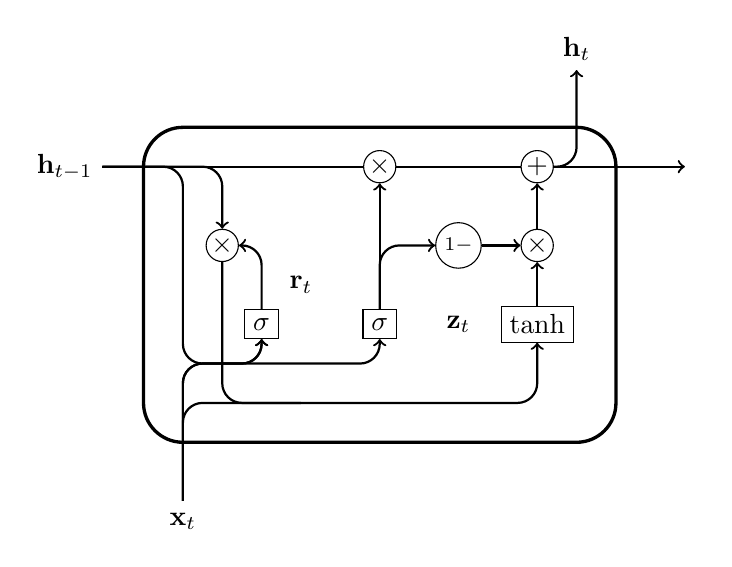
\begin{tikzpicture}[
    % Styles
    cell/.style={% For the main box
        rectangle, 
        rounded corners=5mm, 
        draw,
        very thick,
        },
    operator/.style={%For operators like +  and  x
        circle,
        draw,
        inner sep=0.5pt,
        minimum height =.2cm,
        },
    function/.style={%For functions
        ellipse,
        draw,
        inner sep=3pt
        },
    ct/.style={% For external inputs and outputs
        circle,
        draw,
        line width = .75pt,
        minimum width=1cm,
        inner sep=1pt,
        },
    gt/.style={% For internal inputs
        rectangle,
        draw,
        minimum width=4mm,
        minimum height=3mm,
        inner sep=3pt
        },
    ArrowC1/.style={% Arrows with rounded corners
        rounded corners=.25cm,
        thick,
        },
    ArrowC2/.style={% Arrows with big rounded corners
        rounded corners=.5cm,
        thick,
        },
    ]
    
   %Start drawing the thing...    
    % Draw the cell: 
    \node [cell, minimum height =4cm, minimum width=6cm] at (0,0){} ;
    
    
	%Draw operators	
	%top row
	\node [operator] (mux1) at (0,1.5) {$\times$};
    \node [operator] (add1) at (2,1.5) {$+$};
    %second row
    \node [operator] (mux2) at (-2, 0.5) {$\times$};
    \node [operator] (mux3) at (2,  0.5) {$\times$};
    \node [operator, inner sep=0pt] (minus) at (1, 0.5) {
    \begin{scriptsize}
    $1-$
    \end{scriptsize}
    };
    %bottom row
    \node [gt] (sigma1) at (-1.5, -0.5) {$\sigma$};
    \node [gt] (sigma2) at (0, -0.5) {$\sigma$};
    \node [gt] (tanh) at (2, -0.5) {$\tanh$};
    
    %draw node to show location of gates
    \node[] (zt) at (1, -0.5) {$\mathbf{z}_t$};
    \node[]  (rt) at (-1, 0) {$\mathbf{r}_t$};
    
  % Draw External inputs
    \node[] (ht-1) at (-4,1.5) {$\mathbf{h}_{t-1}$};
    \node[outer sep=1] (xt) at (-2.5,-3) {$\mathbf{x}_t$};

    % Draw External outputs
    \node[] (out) at (4,1.5) {};
    \node[] (ht) at (2.5,3) {$\mathbf{h}_t$};
    
   % Draw Arrows
   % input
	\draw [ArrowC2] (ht-1) -- (mux1) ;
	\draw [->, ArrowC1] (ht-1) -| (mux2);
	\draw[->, ArrowC1] (ht-1) -| (-2.5, -1) -| (sigma1);
	\draw[->, ArrowC1] (xt.north) -| (-2.5, -1) -| (sigma1);
	\draw[->, ArrowC1] (xt.north) |- (-1.5, -1.5) -|(tanh);
	\draw[->, ArrowC1] (xt.north) -| (-2.5, -1) -| (sigma2);
   
	% Internal   
	\draw[->, ArrowC1] (mux1) -- (add1) -- (out);
	\draw[ArrowC1] (mux2) |- (-1,-1.5); 
	\draw[->, ArrowC1] (sigma1) |- (mux2);
	\draw[->, ArrowC1] (sigma2) -- (mux1);
	\draw[->, ArrowC1] (sigma2) |- (minus);
	\draw[->, ArrowC1] (minus) -- (mux3);
	\draw[->, ArrowC1] (tanh) -- (mux3);
	\draw[->, ArrowC1] (mux3) -- (add1);
   
   %Output
   \draw[->, ArrowC1] (add1) -| (ht);
    
\end{tikzpicture}
\caption{Gated Recurrent Unit}
\label{fig:gru}
\end{figure}


\section{Feature Selection}
\label{sec:fs_algos}

Feature Selection is pivotal in machine learning, particularly when dealing with high-dimensional data. It serves the primary objectives of improving model performance by mitigating the 'curse of dimensionality,' enhancing predictive accuracy, and reducing overfitting. By eliminating irrelevant or redundant features, the model's generalization capacity is enhanced, contributing to model interpretability and potentially reducing training times.
Feature selection methods can be broadly categorized into three distinct types \cite{jovicReviewFeatureSelection2015}:
\begin{description}

\item[Filter Methods] These methods rely on model-invariant information, such as feature-class label correlation. They are computationally efficient and typically do not require user input in form of hyperparameters, but may not capture complex relationships within the data.

\item[Wrapper Methods] Wrapper methods train models iteratively on various feature subsets, incurring a higher computational cost but enabling the detection of interactions among variables.

\item[Embedded Methods] These methods perform inherent feature selection, often as an integral part of the modeling process. Tree-based models, such as Decision Trees and Gradient Boosted Trees, typically employ feature selection based on metrics like the Gini index or entropy.
\end{description}


\subsection{Pearson's Correlation Coefficient}
\label{ssec:pearsons}
\Ac{pcc} is a statistical measure widely used to evaluate the linear relationship between two variables. 
Specifically, we consider its application in the context of feature selection in machine learning, where it is used to assess the linear correlation between input features and the target variable. 
We regard the input vector $\mathbf{x}$ as a manifestation of an underlying, unknown distribution. 
Here, $X_i$ represents the random variable corresponding to the $i^{\text{th}}$ component of $\mathbf{x}$, and $y$ is the target value, viewed as a realization of the random variable $Y$ \cite{guyonIntroductionVariableFeature}. 
\Ac{pcc} is employed to quantify the linear correlation between these two random variables. It is defined by the formula:
\begin{equation}
R(i) = \frac{\text{cov}(X_i, Y)}{\sqrt{\text{var}(X_i) \cdot \text{var}(Y)}},
\end{equation}
where $\text{cov}(X_i, Y)$ is the covariance between $X_i$ and $Y$, and $\text{var}(X_i)$ and $\text{var}(Y)$ are the variances of $X_i$ and $Y$, respectively \cite{chandrashekarSurveyFeatureSelection2014}.
$R(i) \in [-1; +1]$ where -1 and +1 are strong negative or positive correlations and 0 indicates no correlation. 
In order to ascertain the significance of the test results, a hypothesis test needs to be performed, with the null hypothesis being that there is no correlation between the feature and the target.
As it is a non-parametric model, there is no need to tune hyperparameters or risk of overfitting.
While simple and effective for identifying linear relationships, \ac{pcc} only captures linear dependencies and might miss non-linear relationships crucial for neural networks.
Despite these limitations, \ac{pcc} remains a valuable tool in feature selection for its simplicity and efficiency in revealing linear correlations.

\subsection{Gradient Boosted Trees}
\label{ssec:gbt}

\Ac{gbt} is an ensemble learning technique that can be used for feature selection. 
The core idea of \ac{gbt} is to build a model in a stage-wise fashion, where each tree incrementally improves upon the previous ones by correcting their errors. 
This process involves training trees sequentially, with each new tree learning to predict the residuals or errors of the previous ensemble of trees.
There are different types of importance, such as the average or total gain across all splits the feature is used in.
The simplest definition is the 'weight', defined as the number of times a feature is used to split the data across all trees \cite{chenXGBoostScalableTree2016}.



\chapter{Data}
\label{chap:data}

Two different datasets need to be constructed: one dataset containing all relevant information prior to the start of the game and one dataset containing only the temporal information from the beginning of the game.


\section{Data Collection}
\label{sec:datacoll}

The data collection process for this study involved a dual-pronged approach, leveraging the extensive resources provided by the Riot Games API alongside a targeted web-scraping strategy.
The resulting raw dataset containing $38,573$ and  $3,972$ matches in the pre-game and in-game datasets respectively, stored in a PostgreSQL Database, reflects a comprehensive compilation of high-rank amateur League of Legends matches.

\paragraph{High-Rank Matches}
The rating system in \ac{lol} groups players into different skill groups, where the lowest is 'Iron' and the highest 'Challenger'.
The two highest ranks,'Grandmaster' and 'Challenger' contain the best 300 and 700 best players on each server.
The exact number of players these tiers depend on the player number in each region (see \cite{riotgamesMasterGrandmasterChallenger2023}).

Similar to the methodology of \citeauthor{zhangPredictionEsportsGame2021}, the focus of data acquisition was directed towards high-rank matches, in which a mix of excellent amateur and professional players play.
High rank matches in this context are defined as having at least one player holding the rank of Master, Grandmaster or Challenger.
These ranks combined account for the top $0.2\%$ of all players \cite{riotgamesRankedTiersDivisions2023}.
Riot Games themselves considers any rank above Diamond 3 as 'Elite' \cite{riotgamesDevBalanceFramework2020}, but we raise this bar just slightly to only include any rank at Master or above.
Due to the fact that for a match to be included in the dataset, only one out of ten players needs to hold one of the aforementioned highest ranks, some slightly lower ranked players are also present in the dataset.

Lower rank matches are not considered due to their higher unpredictability as less skilled players should make huge, game-changing mistakes way more often.
This higher unpredictability could make it harder for the model to learn.

Pro matches, defined as professional players playing with their respective teams in an esport tournament or league, are not included as they are not available through the official Riot Games API.
Professional players are still included in the dataset, but only if they played regular, non-tournament games.

\paragraph{Riot Games API}
The primary source of data stemmed from the Riot Games API \cite{RiotDeveloperPortal}, a comprehensive repository of information pertaining to League of Legends gameplay.
The Riot Games API provided access to a plethora of essential data points, including champion statistics, general match information, timeline details, and player-specific information.
These variables collectively form a comprehensive and multifaceted dataset crucial for the development of an effective predictive model.
\paragraph{Other Data Sources}
However, not all pertinent data were available directly from the Riot Games API.
These include the general winning chance of each champion and statistics on how each player performs on each relevant champion.
To address this limitation, additional relevant information was gathered by using web scraping on u.gg \cite{GGBestLeague}.
\paragraph{Regions}
Multiple regions were included in the data collection process, including Europe West (EUW), Europe Nordic \& East (EUN), Korea (KR), and North America (NA).
This regional diversity contributes to the model's generalizability across different player bases and playing styles.
\paragraph{Period of Time}
All matches included in the dataset were played in season 13 and on patch 20.
It is important that all matches are played on the same patch, as a patch may cause major shifts in the balance of the game, thus making certain strategies and champions way better than others.



\section{Dataset Properties}
\label{sec:dataprop}

The pre-game dataset encompasses a total of 38,573 matches, while the in-game dataset contains 28,809 matches.
Below, the pre-game dataset is presented in more detail, as the smaller in-game dataset is a random sampling from the pre-game dataset.
\paragraph{Region Distribution}
The dataset is primarily comprised of matches from three major regions: North America, Western Europe, and South Korea, which collectively constitute the vast majority of matches in our dataset. 
It is important to note that due to a lack of official data pertaining to the number of games played or the number of players in each region, we are unable to conclusively verify whether the distribution of matches within our dataset aligns with the true underlying distribution of games played per region.
The major regions in the dataset are the same regions getting guaranteed spots at the world championship \cite{2023LeagueLegends2023} with the exception of china, whose matches are not available through the Riot Games API.
Consequently, it is reasonable to assume that this composition approximately mirrors the real-world distribution of matches.
A visual representation of the distribution of matches across regions is provided in Figure \ref{fig:platformId}.


\begin{figure}[ht]
%% Creator: Matplotlib, PGF backend
%%
%% To include the figure in your LaTeX document, write
%%   \input{<filename>.pgf}
%%
%% Make sure the required packages are loaded in your preamble
%%   \usepackage{pgf}
%%
%% Also ensure that all the required font packages are loaded; for instance,
%% the lmodern package is sometimes necessary when using math font.
%%   \usepackage{lmodern}
%%
%% Figures using additional raster images can only be included by \input if
%% they are in the same directory as the main LaTeX file. For loading figures
%% from other directories you can use the `import` package
%%   \usepackage{import}
%%
%% and then include the figures with
%%   \import{<path to file>}{<filename>.pgf}
%%
%% Matplotlib used the following preamble
%%   
%%   \usepackage{fontspec}
%%   \setmainfont{DejaVuSerif.ttf}[Path=\detokenize{/Users/admin/opt/miniconda3/envs/Leaguify/lib/python3.10/site-packages/matplotlib/mpl-data/fonts/ttf/}]
%%   \setsansfont{Arial.ttf}[Path=\detokenize{/System/Library/Fonts/Supplemental/}]
%%   \setmonofont{DejaVuSansMono.ttf}[Path=\detokenize{/Users/admin/opt/miniconda3/envs/Leaguify/lib/python3.10/site-packages/matplotlib/mpl-data/fonts/ttf/}]
%%   \makeatletter\@ifpackageloaded{underscore}{}{\usepackage[strings]{underscore}}\makeatother
%%
\begingroup%
\makeatletter%
\begin{pgfpicture}%
\pgfpathrectangle{\pgfpointorigin}{\pgfqpoint{6.268788in}{4.714041in}}%
\pgfusepath{use as bounding box, clip}%
\begin{pgfscope}%
\pgfsetbuttcap%
\pgfsetmiterjoin%
\definecolor{currentfill}{rgb}{1.000000,1.000000,1.000000}%
\pgfsetfillcolor{currentfill}%
\pgfsetlinewidth{0.000000pt}%
\definecolor{currentstroke}{rgb}{1.000000,1.000000,1.000000}%
\pgfsetstrokecolor{currentstroke}%
\pgfsetdash{}{0pt}%
\pgfpathmoveto{\pgfqpoint{0.000000in}{0.000000in}}%
\pgfpathlineto{\pgfqpoint{6.268788in}{0.000000in}}%
\pgfpathlineto{\pgfqpoint{6.268788in}{4.714041in}}%
\pgfpathlineto{\pgfqpoint{0.000000in}{4.714041in}}%
\pgfpathlineto{\pgfqpoint{0.000000in}{0.000000in}}%
\pgfpathclose%
\pgfusepath{fill}%
\end{pgfscope}%
\begin{pgfscope}%
\pgfsetbuttcap%
\pgfsetmiterjoin%
\definecolor{currentfill}{rgb}{0.917647,0.917647,0.949020}%
\pgfsetfillcolor{currentfill}%
\pgfsetlinewidth{0.000000pt}%
\definecolor{currentstroke}{rgb}{0.000000,0.000000,0.000000}%
\pgfsetstrokecolor{currentstroke}%
\pgfsetstrokeopacity{0.000000}%
\pgfsetdash{}{0pt}%
\pgfpathmoveto{\pgfqpoint{1.715316in}{0.506819in}}%
\pgfpathlineto{\pgfqpoint{6.168788in}{0.506819in}}%
\pgfpathlineto{\pgfqpoint{6.168788in}{4.614041in}}%
\pgfpathlineto{\pgfqpoint{1.715316in}{4.614041in}}%
\pgfpathlineto{\pgfqpoint{1.715316in}{0.506819in}}%
\pgfpathclose%
\pgfusepath{fill}%
\end{pgfscope}%
\begin{pgfscope}%
\pgfpathrectangle{\pgfqpoint{1.715316in}{0.506819in}}{\pgfqpoint{4.453472in}{4.107222in}}%
\pgfusepath{clip}%
\pgfsetroundcap%
\pgfsetroundjoin%
\pgfsetlinewidth{0.803000pt}%
\definecolor{currentstroke}{rgb}{1.000000,1.000000,1.000000}%
\pgfsetstrokecolor{currentstroke}%
\pgfsetdash{}{0pt}%
\pgfpathmoveto{\pgfqpoint{1.715316in}{0.506819in}}%
\pgfpathlineto{\pgfqpoint{1.715316in}{4.614041in}}%
\pgfusepath{stroke}%
\end{pgfscope}%
\begin{pgfscope}%
\definecolor{textcolor}{rgb}{0.150000,0.150000,0.150000}%
\pgfsetstrokecolor{textcolor}%
\pgfsetfillcolor{textcolor}%
\pgftext[x=1.715316in,y=0.409597in,,top]{\color{textcolor}\sffamily\fontsize{10.000000}{12.000000}\selectfont 0}%
\end{pgfscope}%
\begin{pgfscope}%
\pgfpathrectangle{\pgfqpoint{1.715316in}{0.506819in}}{\pgfqpoint{4.453472in}{4.107222in}}%
\pgfusepath{clip}%
\pgfsetroundcap%
\pgfsetroundjoin%
\pgfsetlinewidth{0.803000pt}%
\definecolor{currentstroke}{rgb}{1.000000,1.000000,1.000000}%
\pgfsetstrokecolor{currentstroke}%
\pgfsetdash{}{0pt}%
\pgfpathmoveto{\pgfqpoint{2.292408in}{0.506819in}}%
\pgfpathlineto{\pgfqpoint{2.292408in}{4.614041in}}%
\pgfusepath{stroke}%
\end{pgfscope}%
\begin{pgfscope}%
\definecolor{textcolor}{rgb}{0.150000,0.150000,0.150000}%
\pgfsetstrokecolor{textcolor}%
\pgfsetfillcolor{textcolor}%
\pgftext[x=2.292408in,y=0.409597in,,top]{\color{textcolor}\sffamily\fontsize{10.000000}{12.000000}\selectfont 2500}%
\end{pgfscope}%
\begin{pgfscope}%
\pgfpathrectangle{\pgfqpoint{1.715316in}{0.506819in}}{\pgfqpoint{4.453472in}{4.107222in}}%
\pgfusepath{clip}%
\pgfsetroundcap%
\pgfsetroundjoin%
\pgfsetlinewidth{0.803000pt}%
\definecolor{currentstroke}{rgb}{1.000000,1.000000,1.000000}%
\pgfsetstrokecolor{currentstroke}%
\pgfsetdash{}{0pt}%
\pgfpathmoveto{\pgfqpoint{2.869501in}{0.506819in}}%
\pgfpathlineto{\pgfqpoint{2.869501in}{4.614041in}}%
\pgfusepath{stroke}%
\end{pgfscope}%
\begin{pgfscope}%
\definecolor{textcolor}{rgb}{0.150000,0.150000,0.150000}%
\pgfsetstrokecolor{textcolor}%
\pgfsetfillcolor{textcolor}%
\pgftext[x=2.869501in,y=0.409597in,,top]{\color{textcolor}\sffamily\fontsize{10.000000}{12.000000}\selectfont 5000}%
\end{pgfscope}%
\begin{pgfscope}%
\pgfpathrectangle{\pgfqpoint{1.715316in}{0.506819in}}{\pgfqpoint{4.453472in}{4.107222in}}%
\pgfusepath{clip}%
\pgfsetroundcap%
\pgfsetroundjoin%
\pgfsetlinewidth{0.803000pt}%
\definecolor{currentstroke}{rgb}{1.000000,1.000000,1.000000}%
\pgfsetstrokecolor{currentstroke}%
\pgfsetdash{}{0pt}%
\pgfpathmoveto{\pgfqpoint{3.446594in}{0.506819in}}%
\pgfpathlineto{\pgfqpoint{3.446594in}{4.614041in}}%
\pgfusepath{stroke}%
\end{pgfscope}%
\begin{pgfscope}%
\definecolor{textcolor}{rgb}{0.150000,0.150000,0.150000}%
\pgfsetstrokecolor{textcolor}%
\pgfsetfillcolor{textcolor}%
\pgftext[x=3.446594in,y=0.409597in,,top]{\color{textcolor}\sffamily\fontsize{10.000000}{12.000000}\selectfont 7500}%
\end{pgfscope}%
\begin{pgfscope}%
\pgfpathrectangle{\pgfqpoint{1.715316in}{0.506819in}}{\pgfqpoint{4.453472in}{4.107222in}}%
\pgfusepath{clip}%
\pgfsetroundcap%
\pgfsetroundjoin%
\pgfsetlinewidth{0.803000pt}%
\definecolor{currentstroke}{rgb}{1.000000,1.000000,1.000000}%
\pgfsetstrokecolor{currentstroke}%
\pgfsetdash{}{0pt}%
\pgfpathmoveto{\pgfqpoint{4.023687in}{0.506819in}}%
\pgfpathlineto{\pgfqpoint{4.023687in}{4.614041in}}%
\pgfusepath{stroke}%
\end{pgfscope}%
\begin{pgfscope}%
\definecolor{textcolor}{rgb}{0.150000,0.150000,0.150000}%
\pgfsetstrokecolor{textcolor}%
\pgfsetfillcolor{textcolor}%
\pgftext[x=4.023687in,y=0.409597in,,top]{\color{textcolor}\sffamily\fontsize{10.000000}{12.000000}\selectfont 10000}%
\end{pgfscope}%
\begin{pgfscope}%
\pgfpathrectangle{\pgfqpoint{1.715316in}{0.506819in}}{\pgfqpoint{4.453472in}{4.107222in}}%
\pgfusepath{clip}%
\pgfsetroundcap%
\pgfsetroundjoin%
\pgfsetlinewidth{0.803000pt}%
\definecolor{currentstroke}{rgb}{1.000000,1.000000,1.000000}%
\pgfsetstrokecolor{currentstroke}%
\pgfsetdash{}{0pt}%
\pgfpathmoveto{\pgfqpoint{4.600780in}{0.506819in}}%
\pgfpathlineto{\pgfqpoint{4.600780in}{4.614041in}}%
\pgfusepath{stroke}%
\end{pgfscope}%
\begin{pgfscope}%
\definecolor{textcolor}{rgb}{0.150000,0.150000,0.150000}%
\pgfsetstrokecolor{textcolor}%
\pgfsetfillcolor{textcolor}%
\pgftext[x=4.600780in,y=0.409597in,,top]{\color{textcolor}\sffamily\fontsize{10.000000}{12.000000}\selectfont 12500}%
\end{pgfscope}%
\begin{pgfscope}%
\pgfpathrectangle{\pgfqpoint{1.715316in}{0.506819in}}{\pgfqpoint{4.453472in}{4.107222in}}%
\pgfusepath{clip}%
\pgfsetroundcap%
\pgfsetroundjoin%
\pgfsetlinewidth{0.803000pt}%
\definecolor{currentstroke}{rgb}{1.000000,1.000000,1.000000}%
\pgfsetstrokecolor{currentstroke}%
\pgfsetdash{}{0pt}%
\pgfpathmoveto{\pgfqpoint{5.177873in}{0.506819in}}%
\pgfpathlineto{\pgfqpoint{5.177873in}{4.614041in}}%
\pgfusepath{stroke}%
\end{pgfscope}%
\begin{pgfscope}%
\definecolor{textcolor}{rgb}{0.150000,0.150000,0.150000}%
\pgfsetstrokecolor{textcolor}%
\pgfsetfillcolor{textcolor}%
\pgftext[x=5.177873in,y=0.409597in,,top]{\color{textcolor}\sffamily\fontsize{10.000000}{12.000000}\selectfont 15000}%
\end{pgfscope}%
\begin{pgfscope}%
\pgfpathrectangle{\pgfqpoint{1.715316in}{0.506819in}}{\pgfqpoint{4.453472in}{4.107222in}}%
\pgfusepath{clip}%
\pgfsetroundcap%
\pgfsetroundjoin%
\pgfsetlinewidth{0.803000pt}%
\definecolor{currentstroke}{rgb}{1.000000,1.000000,1.000000}%
\pgfsetstrokecolor{currentstroke}%
\pgfsetdash{}{0pt}%
\pgfpathmoveto{\pgfqpoint{5.754966in}{0.506819in}}%
\pgfpathlineto{\pgfqpoint{5.754966in}{4.614041in}}%
\pgfusepath{stroke}%
\end{pgfscope}%
\begin{pgfscope}%
\definecolor{textcolor}{rgb}{0.150000,0.150000,0.150000}%
\pgfsetstrokecolor{textcolor}%
\pgfsetfillcolor{textcolor}%
\pgftext[x=5.754966in,y=0.409597in,,top]{\color{textcolor}\sffamily\fontsize{10.000000}{12.000000}\selectfont 17500}%
\end{pgfscope}%
\begin{pgfscope}%
\definecolor{textcolor}{rgb}{0.150000,0.150000,0.150000}%
\pgfsetstrokecolor{textcolor}%
\pgfsetfillcolor{textcolor}%
\pgftext[x=3.942052in,y=0.227021in,,top]{\color{textcolor}\sffamily\fontsize{10.000000}{12.000000}\selectfont Count}%
\end{pgfscope}%
\begin{pgfscope}%
\definecolor{textcolor}{rgb}{0.150000,0.150000,0.150000}%
\pgfsetstrokecolor{textcolor}%
\pgfsetfillcolor{textcolor}%
\pgftext[x=1.270803in, y=4.153609in, left, base]{\color{textcolor}\sffamily\fontsize{10.000000}{12.000000}\selectfont Brazil}%
\end{pgfscope}%
\begin{pgfscope}%
\definecolor{textcolor}{rgb}{0.150000,0.150000,0.150000}%
\pgfsetstrokecolor{textcolor}%
\pgfsetfillcolor{textcolor}%
\pgftext[x=0.282576in, y=3.331317in, left, base]{\color{textcolor}\sffamily\fontsize{10.000000}{12.000000}\selectfont Europe Nordic \& East}%
\end{pgfscope}%
\begin{pgfscope}%
\definecolor{textcolor}{rgb}{0.150000,0.150000,0.150000}%
\pgfsetstrokecolor{textcolor}%
\pgfsetfillcolor{textcolor}%
\pgftext[x=0.817787in, y=2.510721in, left, base]{\color{textcolor}\sffamily\fontsize{10.000000}{12.000000}\selectfont Europe West}%
\end{pgfscope}%
\begin{pgfscope}%
\definecolor{textcolor}{rgb}{0.150000,0.150000,0.150000}%
\pgfsetstrokecolor{textcolor}%
\pgfsetfillcolor{textcolor}%
\pgftext[x=1.247474in, y=1.689276in, left, base]{\color{textcolor}\sffamily\fontsize{10.000000}{12.000000}\selectfont Korea}%
\end{pgfscope}%
\begin{pgfscope}%
\definecolor{textcolor}{rgb}{0.150000,0.150000,0.150000}%
\pgfsetstrokecolor{textcolor}%
\pgfsetfillcolor{textcolor}%
\pgftext[x=0.730507in, y=0.867832in, left, base]{\color{textcolor}\sffamily\fontsize{10.000000}{12.000000}\selectfont North America}%
\end{pgfscope}%
\begin{pgfscope}%
\definecolor{textcolor}{rgb}{0.150000,0.150000,0.150000}%
\pgfsetstrokecolor{textcolor}%
\pgfsetfillcolor{textcolor}%
\pgftext[x=0.227021in,y=2.560430in,,bottom,rotate=90.000000]{\color{textcolor}\sffamily\fontsize{10.000000}{12.000000}\selectfont Platform ID}%
\end{pgfscope}%
\begin{pgfscope}%
\pgfpathrectangle{\pgfqpoint{1.715316in}{0.506819in}}{\pgfqpoint{4.453472in}{4.107222in}}%
\pgfusepath{clip}%
\pgfsetbuttcap%
\pgfsetmiterjoin%
\definecolor{currentfill}{rgb}{0.194608,0.453431,0.632843}%
\pgfsetfillcolor{currentfill}%
\pgfsetlinewidth{1.003750pt}%
\definecolor{currentstroke}{rgb}{1.000000,1.000000,1.000000}%
\pgfsetstrokecolor{currentstroke}%
\pgfsetdash{}{0pt}%
\pgfpathmoveto{\pgfqpoint{1.715316in}{4.531897in}}%
\pgfpathlineto{\pgfqpoint{2.122974in}{4.531897in}}%
\pgfpathlineto{\pgfqpoint{2.122974in}{3.874741in}}%
\pgfpathlineto{\pgfqpoint{1.715316in}{3.874741in}}%
\pgfpathlineto{\pgfqpoint{1.715316in}{4.531897in}}%
\pgfpathclose%
\pgfusepath{stroke,fill}%
\end{pgfscope}%
\begin{pgfscope}%
\pgfpathrectangle{\pgfqpoint{1.715316in}{0.506819in}}{\pgfqpoint{4.453472in}{4.107222in}}%
\pgfusepath{clip}%
\pgfsetbuttcap%
\pgfsetmiterjoin%
\definecolor{currentfill}{rgb}{0.881863,0.505392,0.173039}%
\pgfsetfillcolor{currentfill}%
\pgfsetlinewidth{1.003750pt}%
\definecolor{currentstroke}{rgb}{1.000000,1.000000,1.000000}%
\pgfsetstrokecolor{currentstroke}%
\pgfsetdash{}{0pt}%
\pgfpathmoveto{\pgfqpoint{1.715316in}{3.710452in}}%
\pgfpathlineto{\pgfqpoint{2.540097in}{3.710452in}}%
\pgfpathlineto{\pgfqpoint{2.540097in}{3.053297in}}%
\pgfpathlineto{\pgfqpoint{1.715316in}{3.053297in}}%
\pgfpathlineto{\pgfqpoint{1.715316in}{3.710452in}}%
\pgfpathclose%
\pgfusepath{stroke,fill}%
\end{pgfscope}%
\begin{pgfscope}%
\pgfpathrectangle{\pgfqpoint{1.715316in}{0.506819in}}{\pgfqpoint{4.453472in}{4.107222in}}%
\pgfusepath{clip}%
\pgfsetbuttcap%
\pgfsetmiterjoin%
\definecolor{currentfill}{rgb}{0.229412,0.570588,0.229412}%
\pgfsetfillcolor{currentfill}%
\pgfsetlinewidth{1.003750pt}%
\definecolor{currentstroke}{rgb}{1.000000,1.000000,1.000000}%
\pgfsetstrokecolor{currentstroke}%
\pgfsetdash{}{0pt}%
\pgfpathmoveto{\pgfqpoint{1.715316in}{2.889008in}}%
\pgfpathlineto{\pgfqpoint{4.651103in}{2.889008in}}%
\pgfpathlineto{\pgfqpoint{4.651103in}{2.231852in}}%
\pgfpathlineto{\pgfqpoint{1.715316in}{2.231852in}}%
\pgfpathlineto{\pgfqpoint{1.715316in}{2.889008in}}%
\pgfpathclose%
\pgfusepath{stroke,fill}%
\end{pgfscope}%
\begin{pgfscope}%
\pgfpathrectangle{\pgfqpoint{1.715316in}{0.506819in}}{\pgfqpoint{4.453472in}{4.107222in}}%
\pgfusepath{clip}%
\pgfsetbuttcap%
\pgfsetmiterjoin%
\definecolor{currentfill}{rgb}{0.753431,0.238725,0.241667}%
\pgfsetfillcolor{currentfill}%
\pgfsetlinewidth{1.003750pt}%
\definecolor{currentstroke}{rgb}{1.000000,1.000000,1.000000}%
\pgfsetstrokecolor{currentstroke}%
\pgfsetdash{}{0pt}%
\pgfpathmoveto{\pgfqpoint{1.715316in}{2.067564in}}%
\pgfpathlineto{\pgfqpoint{5.161714in}{2.067564in}}%
\pgfpathlineto{\pgfqpoint{5.161714in}{1.410408in}}%
\pgfpathlineto{\pgfqpoint{1.715316in}{1.410408in}}%
\pgfpathlineto{\pgfqpoint{1.715316in}{2.067564in}}%
\pgfpathclose%
\pgfusepath{stroke,fill}%
\end{pgfscope}%
\begin{pgfscope}%
\pgfpathrectangle{\pgfqpoint{1.715316in}{0.506819in}}{\pgfqpoint{4.453472in}{4.107222in}}%
\pgfusepath{clip}%
\pgfsetbuttcap%
\pgfsetmiterjoin%
\definecolor{currentfill}{rgb}{0.578431,0.446078,0.699020}%
\pgfsetfillcolor{currentfill}%
\pgfsetlinewidth{1.003750pt}%
\definecolor{currentstroke}{rgb}{1.000000,1.000000,1.000000}%
\pgfsetstrokecolor{currentstroke}%
\pgfsetdash{}{0pt}%
\pgfpathmoveto{\pgfqpoint{1.715316in}{1.246119in}}%
\pgfpathlineto{\pgfqpoint{5.956718in}{1.246119in}}%
\pgfpathlineto{\pgfqpoint{5.956718in}{0.588964in}}%
\pgfpathlineto{\pgfqpoint{1.715316in}{0.588964in}}%
\pgfpathlineto{\pgfqpoint{1.715316in}{1.246119in}}%
\pgfpathclose%
\pgfusepath{stroke,fill}%
\end{pgfscope}%
\begin{pgfscope}%
\pgfsetrectcap%
\pgfsetmiterjoin%
\pgfsetlinewidth{0.803000pt}%
\definecolor{currentstroke}{rgb}{1.000000,1.000000,1.000000}%
\pgfsetstrokecolor{currentstroke}%
\pgfsetdash{}{0pt}%
\pgfpathmoveto{\pgfqpoint{1.715316in}{0.506819in}}%
\pgfpathlineto{\pgfqpoint{1.715316in}{4.614041in}}%
\pgfusepath{stroke}%
\end{pgfscope}%
\begin{pgfscope}%
\pgfsetrectcap%
\pgfsetmiterjoin%
\pgfsetlinewidth{0.803000pt}%
\definecolor{currentstroke}{rgb}{1.000000,1.000000,1.000000}%
\pgfsetstrokecolor{currentstroke}%
\pgfsetdash{}{0pt}%
\pgfpathmoveto{\pgfqpoint{6.168788in}{0.506819in}}%
\pgfpathlineto{\pgfqpoint{6.168788in}{4.614041in}}%
\pgfusepath{stroke}%
\end{pgfscope}%
\begin{pgfscope}%
\pgfsetrectcap%
\pgfsetmiterjoin%
\pgfsetlinewidth{0.803000pt}%
\definecolor{currentstroke}{rgb}{1.000000,1.000000,1.000000}%
\pgfsetstrokecolor{currentstroke}%
\pgfsetdash{}{0pt}%
\pgfpathmoveto{\pgfqpoint{1.715316in}{0.506819in}}%
\pgfpathlineto{\pgfqpoint{6.168788in}{0.506819in}}%
\pgfusepath{stroke}%
\end{pgfscope}%
\begin{pgfscope}%
\pgfsetrectcap%
\pgfsetmiterjoin%
\pgfsetlinewidth{0.803000pt}%
\definecolor{currentstroke}{rgb}{1.000000,1.000000,1.000000}%
\pgfsetstrokecolor{currentstroke}%
\pgfsetdash{}{0pt}%
\pgfpathmoveto{\pgfqpoint{1.715316in}{4.614041in}}%
\pgfpathlineto{\pgfqpoint{6.168788in}{4.614041in}}%
\pgfusepath{stroke}%
\end{pgfscope}%
\end{pgfpicture}%
\makeatother%
\endgroup%

\caption{Region distribution}
\label{fig:platformId}
\end{figure}

\paragraph{Game length}
As only matches with a game length of at least 16 minutes are collected, the shortest match is 16 minutes long, while the longest game is $59.62$ minutes long.
The average match length is $27.50$ minutes.
Figure \ref{fig:gameDuration} graphically illustrates the distribution of game durations. 
Notably, the histogram reveals a prominent spike at the 16-minute mark.
This spike corresponds to the earliest possible conclusion time for a match, as League of Legends prohibits surrendering prior to the 15th minute of gameplay. In instances where an entire team collectively acknowledges the futility of their chances of victory, a surrender may be initiated at the 15-minute threshold.
If a simple majority of team members want to surrender, they have to wait until the 20th minute.
However, should a simple majority of team members decide to surrender, they must adhere to a 20-minute waiting period before being able to do so. 
Consequently, this unique feature of the game's mechanics clarifies the relatively diminished frequency of matches ending in the 17th to 19th-minute range within our dataset.

\begin{figure}[ht]
%% Creator: Matplotlib, PGF backend
%%
%% To include the figure in your LaTeX document, write
%%   \input{<filename>.pgf}
%%
%% Make sure the required packages are loaded in your preamble
%%   \usepackage{pgf}
%%
%% Also ensure that all the required font packages are loaded; for instance,
%% the lmodern package is sometimes necessary when using math font.
%%   \usepackage{lmodern}
%%
%% Figures using additional raster images can only be included by \input if
%% they are in the same directory as the main LaTeX file. For loading figures
%% from other directories you can use the `import` package
%%   \usepackage{import}
%%
%% and then include the figures with
%%   \import{<path to file>}{<filename>.pgf}
%%
%% Matplotlib used the following preamble
%%   
%%   \usepackage{fontspec}
%%   \setmainfont{DejaVuSerif.ttf}[Path=\detokenize{C:/Users/morit/AppData/Local/pypoetry/Cache/virtualenvs/leaguify-VaCbhr8h-py3.11/Lib/site-packages/matplotlib/mpl-data/fonts/ttf/}]
%%   \setsansfont{arial.ttf}[Path=\detokenize{C:/Windows/Fonts/}]
%%   \setmonofont{DejaVuSansMono.ttf}[Path=\detokenize{C:/Users/morit/AppData/Local/pypoetry/Cache/virtualenvs/leaguify-VaCbhr8h-py3.11/Lib/site-packages/matplotlib/mpl-data/fonts/ttf/}]
%%   \makeatletter\@ifpackageloaded{underscore}{}{\usepackage[strings]{underscore}}\makeatother
%%
\begingroup%
\makeatletter%
\begin{pgfpicture}%
\pgfpathrectangle{\pgfpointorigin}{\pgfqpoint{6.400000in}{4.800000in}}%
\pgfusepath{use as bounding box, clip}%
\begin{pgfscope}%
\pgfsetbuttcap%
\pgfsetmiterjoin%
\definecolor{currentfill}{rgb}{1.000000,1.000000,1.000000}%
\pgfsetfillcolor{currentfill}%
\pgfsetlinewidth{0.000000pt}%
\definecolor{currentstroke}{rgb}{1.000000,1.000000,1.000000}%
\pgfsetstrokecolor{currentstroke}%
\pgfsetdash{}{0pt}%
\pgfpathmoveto{\pgfqpoint{0.000000in}{0.000000in}}%
\pgfpathlineto{\pgfqpoint{6.400000in}{0.000000in}}%
\pgfpathlineto{\pgfqpoint{6.400000in}{4.800000in}}%
\pgfpathlineto{\pgfqpoint{0.000000in}{4.800000in}}%
\pgfpathlineto{\pgfqpoint{0.000000in}{0.000000in}}%
\pgfpathclose%
\pgfusepath{fill}%
\end{pgfscope}%
\begin{pgfscope}%
\pgfsetbuttcap%
\pgfsetmiterjoin%
\definecolor{currentfill}{rgb}{0.917647,0.917647,0.949020}%
\pgfsetfillcolor{currentfill}%
\pgfsetlinewidth{0.000000pt}%
\definecolor{currentstroke}{rgb}{0.000000,0.000000,0.000000}%
\pgfsetstrokecolor{currentstroke}%
\pgfsetstrokeopacity{0.000000}%
\pgfsetdash{}{0pt}%
\pgfpathmoveto{\pgfqpoint{0.800000in}{0.528000in}}%
\pgfpathlineto{\pgfqpoint{5.760000in}{0.528000in}}%
\pgfpathlineto{\pgfqpoint{5.760000in}{4.224000in}}%
\pgfpathlineto{\pgfqpoint{0.800000in}{4.224000in}}%
\pgfpathlineto{\pgfqpoint{0.800000in}{0.528000in}}%
\pgfpathclose%
\pgfusepath{fill}%
\end{pgfscope}%
\begin{pgfscope}%
\pgfpathrectangle{\pgfqpoint{0.800000in}{0.528000in}}{\pgfqpoint{4.960000in}{3.696000in}}%
\pgfusepath{clip}%
\pgfsetroundcap%
\pgfsetroundjoin%
\pgfsetlinewidth{0.803000pt}%
\definecolor{currentstroke}{rgb}{1.000000,1.000000,1.000000}%
\pgfsetstrokecolor{currentstroke}%
\pgfsetdash{}{0pt}%
\pgfpathmoveto{\pgfqpoint{1.438975in}{0.528000in}}%
\pgfpathlineto{\pgfqpoint{1.438975in}{4.224000in}}%
\pgfusepath{stroke}%
\end{pgfscope}%
\begin{pgfscope}%
\definecolor{textcolor}{rgb}{0.150000,0.150000,0.150000}%
\pgfsetstrokecolor{textcolor}%
\pgfsetfillcolor{textcolor}%
\pgftext[x=1.438975in,y=0.430778in,,top]{\color{textcolor}\sffamily\fontsize{10.000000}{12.000000}\selectfont 20}%
\end{pgfscope}%
\begin{pgfscope}%
\pgfpathrectangle{\pgfqpoint{0.800000in}{0.528000in}}{\pgfqpoint{4.960000in}{3.696000in}}%
\pgfusepath{clip}%
\pgfsetroundcap%
\pgfsetroundjoin%
\pgfsetlinewidth{0.803000pt}%
\definecolor{currentstroke}{rgb}{1.000000,1.000000,1.000000}%
\pgfsetstrokecolor{currentstroke}%
\pgfsetdash{}{0pt}%
\pgfpathmoveto{\pgfqpoint{2.472775in}{0.528000in}}%
\pgfpathlineto{\pgfqpoint{2.472775in}{4.224000in}}%
\pgfusepath{stroke}%
\end{pgfscope}%
\begin{pgfscope}%
\definecolor{textcolor}{rgb}{0.150000,0.150000,0.150000}%
\pgfsetstrokecolor{textcolor}%
\pgfsetfillcolor{textcolor}%
\pgftext[x=2.472775in,y=0.430778in,,top]{\color{textcolor}\sffamily\fontsize{10.000000}{12.000000}\selectfont 30}%
\end{pgfscope}%
\begin{pgfscope}%
\pgfpathrectangle{\pgfqpoint{0.800000in}{0.528000in}}{\pgfqpoint{4.960000in}{3.696000in}}%
\pgfusepath{clip}%
\pgfsetroundcap%
\pgfsetroundjoin%
\pgfsetlinewidth{0.803000pt}%
\definecolor{currentstroke}{rgb}{1.000000,1.000000,1.000000}%
\pgfsetstrokecolor{currentstroke}%
\pgfsetdash{}{0pt}%
\pgfpathmoveto{\pgfqpoint{3.506574in}{0.528000in}}%
\pgfpathlineto{\pgfqpoint{3.506574in}{4.224000in}}%
\pgfusepath{stroke}%
\end{pgfscope}%
\begin{pgfscope}%
\definecolor{textcolor}{rgb}{0.150000,0.150000,0.150000}%
\pgfsetstrokecolor{textcolor}%
\pgfsetfillcolor{textcolor}%
\pgftext[x=3.506574in,y=0.430778in,,top]{\color{textcolor}\sffamily\fontsize{10.000000}{12.000000}\selectfont 40}%
\end{pgfscope}%
\begin{pgfscope}%
\pgfpathrectangle{\pgfqpoint{0.800000in}{0.528000in}}{\pgfqpoint{4.960000in}{3.696000in}}%
\pgfusepath{clip}%
\pgfsetroundcap%
\pgfsetroundjoin%
\pgfsetlinewidth{0.803000pt}%
\definecolor{currentstroke}{rgb}{1.000000,1.000000,1.000000}%
\pgfsetstrokecolor{currentstroke}%
\pgfsetdash{}{0pt}%
\pgfpathmoveto{\pgfqpoint{4.540374in}{0.528000in}}%
\pgfpathlineto{\pgfqpoint{4.540374in}{4.224000in}}%
\pgfusepath{stroke}%
\end{pgfscope}%
\begin{pgfscope}%
\definecolor{textcolor}{rgb}{0.150000,0.150000,0.150000}%
\pgfsetstrokecolor{textcolor}%
\pgfsetfillcolor{textcolor}%
\pgftext[x=4.540374in,y=0.430778in,,top]{\color{textcolor}\sffamily\fontsize{10.000000}{12.000000}\selectfont 50}%
\end{pgfscope}%
\begin{pgfscope}%
\pgfpathrectangle{\pgfqpoint{0.800000in}{0.528000in}}{\pgfqpoint{4.960000in}{3.696000in}}%
\pgfusepath{clip}%
\pgfsetroundcap%
\pgfsetroundjoin%
\pgfsetlinewidth{0.803000pt}%
\definecolor{currentstroke}{rgb}{1.000000,1.000000,1.000000}%
\pgfsetstrokecolor{currentstroke}%
\pgfsetdash{}{0pt}%
\pgfpathmoveto{\pgfqpoint{5.574174in}{0.528000in}}%
\pgfpathlineto{\pgfqpoint{5.574174in}{4.224000in}}%
\pgfusepath{stroke}%
\end{pgfscope}%
\begin{pgfscope}%
\definecolor{textcolor}{rgb}{0.150000,0.150000,0.150000}%
\pgfsetstrokecolor{textcolor}%
\pgfsetfillcolor{textcolor}%
\pgftext[x=5.574174in,y=0.430778in,,top]{\color{textcolor}\sffamily\fontsize{10.000000}{12.000000}\selectfont 60}%
\end{pgfscope}%
\begin{pgfscope}%
\definecolor{textcolor}{rgb}{0.150000,0.150000,0.150000}%
\pgfsetstrokecolor{textcolor}%
\pgfsetfillcolor{textcolor}%
\pgftext[x=3.280000in,y=0.248202in,,top]{\color{textcolor}\sffamily\fontsize{10.000000}{12.000000}\selectfont Game duration in minutes}%
\end{pgfscope}%
\begin{pgfscope}%
\pgfpathrectangle{\pgfqpoint{0.800000in}{0.528000in}}{\pgfqpoint{4.960000in}{3.696000in}}%
\pgfusepath{clip}%
\pgfsetroundcap%
\pgfsetroundjoin%
\pgfsetlinewidth{0.803000pt}%
\definecolor{currentstroke}{rgb}{1.000000,1.000000,1.000000}%
\pgfsetstrokecolor{currentstroke}%
\pgfsetdash{}{0pt}%
\pgfpathmoveto{\pgfqpoint{0.800000in}{0.528000in}}%
\pgfpathlineto{\pgfqpoint{5.760000in}{0.528000in}}%
\pgfusepath{stroke}%
\end{pgfscope}%
\begin{pgfscope}%
\definecolor{textcolor}{rgb}{0.150000,0.150000,0.150000}%
\pgfsetstrokecolor{textcolor}%
\pgfsetfillcolor{textcolor}%
\pgftext[x=0.625534in, y=0.478290in, left, base]{\color{textcolor}\sffamily\fontsize{10.000000}{12.000000}\selectfont 0}%
\end{pgfscope}%
\begin{pgfscope}%
\pgfpathrectangle{\pgfqpoint{0.800000in}{0.528000in}}{\pgfqpoint{4.960000in}{3.696000in}}%
\pgfusepath{clip}%
\pgfsetroundcap%
\pgfsetroundjoin%
\pgfsetlinewidth{0.803000pt}%
\definecolor{currentstroke}{rgb}{1.000000,1.000000,1.000000}%
\pgfsetstrokecolor{currentstroke}%
\pgfsetdash{}{0pt}%
\pgfpathmoveto{\pgfqpoint{0.800000in}{0.970485in}}%
\pgfpathlineto{\pgfqpoint{5.760000in}{0.970485in}}%
\pgfusepath{stroke}%
\end{pgfscope}%
\begin{pgfscope}%
\definecolor{textcolor}{rgb}{0.150000,0.150000,0.150000}%
\pgfsetstrokecolor{textcolor}%
\pgfsetfillcolor{textcolor}%
\pgftext[x=0.471048in, y=0.920775in, left, base]{\color{textcolor}\sffamily\fontsize{10.000000}{12.000000}\selectfont 500}%
\end{pgfscope}%
\begin{pgfscope}%
\pgfpathrectangle{\pgfqpoint{0.800000in}{0.528000in}}{\pgfqpoint{4.960000in}{3.696000in}}%
\pgfusepath{clip}%
\pgfsetroundcap%
\pgfsetroundjoin%
\pgfsetlinewidth{0.803000pt}%
\definecolor{currentstroke}{rgb}{1.000000,1.000000,1.000000}%
\pgfsetstrokecolor{currentstroke}%
\pgfsetdash{}{0pt}%
\pgfpathmoveto{\pgfqpoint{0.800000in}{1.412970in}}%
\pgfpathlineto{\pgfqpoint{5.760000in}{1.412970in}}%
\pgfusepath{stroke}%
\end{pgfscope}%
\begin{pgfscope}%
\definecolor{textcolor}{rgb}{0.150000,0.150000,0.150000}%
\pgfsetstrokecolor{textcolor}%
\pgfsetfillcolor{textcolor}%
\pgftext[x=0.393804in, y=1.363260in, left, base]{\color{textcolor}\sffamily\fontsize{10.000000}{12.000000}\selectfont 1000}%
\end{pgfscope}%
\begin{pgfscope}%
\pgfpathrectangle{\pgfqpoint{0.800000in}{0.528000in}}{\pgfqpoint{4.960000in}{3.696000in}}%
\pgfusepath{clip}%
\pgfsetroundcap%
\pgfsetroundjoin%
\pgfsetlinewidth{0.803000pt}%
\definecolor{currentstroke}{rgb}{1.000000,1.000000,1.000000}%
\pgfsetstrokecolor{currentstroke}%
\pgfsetdash{}{0pt}%
\pgfpathmoveto{\pgfqpoint{0.800000in}{1.855455in}}%
\pgfpathlineto{\pgfqpoint{5.760000in}{1.855455in}}%
\pgfusepath{stroke}%
\end{pgfscope}%
\begin{pgfscope}%
\definecolor{textcolor}{rgb}{0.150000,0.150000,0.150000}%
\pgfsetstrokecolor{textcolor}%
\pgfsetfillcolor{textcolor}%
\pgftext[x=0.393804in, y=1.805745in, left, base]{\color{textcolor}\sffamily\fontsize{10.000000}{12.000000}\selectfont 1500}%
\end{pgfscope}%
\begin{pgfscope}%
\pgfpathrectangle{\pgfqpoint{0.800000in}{0.528000in}}{\pgfqpoint{4.960000in}{3.696000in}}%
\pgfusepath{clip}%
\pgfsetroundcap%
\pgfsetroundjoin%
\pgfsetlinewidth{0.803000pt}%
\definecolor{currentstroke}{rgb}{1.000000,1.000000,1.000000}%
\pgfsetstrokecolor{currentstroke}%
\pgfsetdash{}{0pt}%
\pgfpathmoveto{\pgfqpoint{0.800000in}{2.297940in}}%
\pgfpathlineto{\pgfqpoint{5.760000in}{2.297940in}}%
\pgfusepath{stroke}%
\end{pgfscope}%
\begin{pgfscope}%
\definecolor{textcolor}{rgb}{0.150000,0.150000,0.150000}%
\pgfsetstrokecolor{textcolor}%
\pgfsetfillcolor{textcolor}%
\pgftext[x=0.393804in, y=2.248230in, left, base]{\color{textcolor}\sffamily\fontsize{10.000000}{12.000000}\selectfont 2000}%
\end{pgfscope}%
\begin{pgfscope}%
\pgfpathrectangle{\pgfqpoint{0.800000in}{0.528000in}}{\pgfqpoint{4.960000in}{3.696000in}}%
\pgfusepath{clip}%
\pgfsetroundcap%
\pgfsetroundjoin%
\pgfsetlinewidth{0.803000pt}%
\definecolor{currentstroke}{rgb}{1.000000,1.000000,1.000000}%
\pgfsetstrokecolor{currentstroke}%
\pgfsetdash{}{0pt}%
\pgfpathmoveto{\pgfqpoint{0.800000in}{2.740425in}}%
\pgfpathlineto{\pgfqpoint{5.760000in}{2.740425in}}%
\pgfusepath{stroke}%
\end{pgfscope}%
\begin{pgfscope}%
\definecolor{textcolor}{rgb}{0.150000,0.150000,0.150000}%
\pgfsetstrokecolor{textcolor}%
\pgfsetfillcolor{textcolor}%
\pgftext[x=0.393804in, y=2.690715in, left, base]{\color{textcolor}\sffamily\fontsize{10.000000}{12.000000}\selectfont 2500}%
\end{pgfscope}%
\begin{pgfscope}%
\pgfpathrectangle{\pgfqpoint{0.800000in}{0.528000in}}{\pgfqpoint{4.960000in}{3.696000in}}%
\pgfusepath{clip}%
\pgfsetroundcap%
\pgfsetroundjoin%
\pgfsetlinewidth{0.803000pt}%
\definecolor{currentstroke}{rgb}{1.000000,1.000000,1.000000}%
\pgfsetstrokecolor{currentstroke}%
\pgfsetdash{}{0pt}%
\pgfpathmoveto{\pgfqpoint{0.800000in}{3.182910in}}%
\pgfpathlineto{\pgfqpoint{5.760000in}{3.182910in}}%
\pgfusepath{stroke}%
\end{pgfscope}%
\begin{pgfscope}%
\definecolor{textcolor}{rgb}{0.150000,0.150000,0.150000}%
\pgfsetstrokecolor{textcolor}%
\pgfsetfillcolor{textcolor}%
\pgftext[x=0.393804in, y=3.133200in, left, base]{\color{textcolor}\sffamily\fontsize{10.000000}{12.000000}\selectfont 3000}%
\end{pgfscope}%
\begin{pgfscope}%
\pgfpathrectangle{\pgfqpoint{0.800000in}{0.528000in}}{\pgfqpoint{4.960000in}{3.696000in}}%
\pgfusepath{clip}%
\pgfsetroundcap%
\pgfsetroundjoin%
\pgfsetlinewidth{0.803000pt}%
\definecolor{currentstroke}{rgb}{1.000000,1.000000,1.000000}%
\pgfsetstrokecolor{currentstroke}%
\pgfsetdash{}{0pt}%
\pgfpathmoveto{\pgfqpoint{0.800000in}{3.625394in}}%
\pgfpathlineto{\pgfqpoint{5.760000in}{3.625394in}}%
\pgfusepath{stroke}%
\end{pgfscope}%
\begin{pgfscope}%
\definecolor{textcolor}{rgb}{0.150000,0.150000,0.150000}%
\pgfsetstrokecolor{textcolor}%
\pgfsetfillcolor{textcolor}%
\pgftext[x=0.393804in, y=3.575685in, left, base]{\color{textcolor}\sffamily\fontsize{10.000000}{12.000000}\selectfont 3500}%
\end{pgfscope}%
\begin{pgfscope}%
\pgfpathrectangle{\pgfqpoint{0.800000in}{0.528000in}}{\pgfqpoint{4.960000in}{3.696000in}}%
\pgfusepath{clip}%
\pgfsetroundcap%
\pgfsetroundjoin%
\pgfsetlinewidth{0.803000pt}%
\definecolor{currentstroke}{rgb}{1.000000,1.000000,1.000000}%
\pgfsetstrokecolor{currentstroke}%
\pgfsetdash{}{0pt}%
\pgfpathmoveto{\pgfqpoint{0.800000in}{4.067879in}}%
\pgfpathlineto{\pgfqpoint{5.760000in}{4.067879in}}%
\pgfusepath{stroke}%
\end{pgfscope}%
\begin{pgfscope}%
\definecolor{textcolor}{rgb}{0.150000,0.150000,0.150000}%
\pgfsetstrokecolor{textcolor}%
\pgfsetfillcolor{textcolor}%
\pgftext[x=0.393804in, y=4.018170in, left, base]{\color{textcolor}\sffamily\fontsize{10.000000}{12.000000}\selectfont 4000}%
\end{pgfscope}%
\begin{pgfscope}%
\definecolor{textcolor}{rgb}{0.150000,0.150000,0.150000}%
\pgfsetstrokecolor{textcolor}%
\pgfsetfillcolor{textcolor}%
\pgftext[x=0.338249in,y=2.376000in,,bottom,rotate=90.000000]{\color{textcolor}\sffamily\fontsize{10.000000}{12.000000}\selectfont Count}%
\end{pgfscope}%
\begin{pgfscope}%
\pgfpathrectangle{\pgfqpoint{0.800000in}{0.528000in}}{\pgfqpoint{4.960000in}{3.696000in}}%
\pgfusepath{clip}%
\pgfsetbuttcap%
\pgfsetmiterjoin%
\definecolor{currentfill}{rgb}{0.121569,0.466667,0.705882}%
\pgfsetfillcolor{currentfill}%
\pgfsetfillopacity{0.500000}%
\pgfsetlinewidth{0.814680pt}%
\definecolor{currentstroke}{rgb}{1.000000,1.000000,1.000000}%
\pgfsetstrokecolor{currentstroke}%
\pgfsetdash{}{0pt}%
\pgfpathmoveto{\pgfqpoint{1.025455in}{0.528000in}}%
\pgfpathlineto{\pgfqpoint{1.138182in}{0.528000in}}%
\pgfpathlineto{\pgfqpoint{1.138182in}{1.788197in}}%
\pgfpathlineto{\pgfqpoint{1.025455in}{1.788197in}}%
\pgfpathlineto{\pgfqpoint{1.025455in}{0.528000in}}%
\pgfpathclose%
\pgfusepath{stroke,fill}%
\end{pgfscope}%
\begin{pgfscope}%
\pgfpathrectangle{\pgfqpoint{0.800000in}{0.528000in}}{\pgfqpoint{4.960000in}{3.696000in}}%
\pgfusepath{clip}%
\pgfsetbuttcap%
\pgfsetmiterjoin%
\definecolor{currentfill}{rgb}{0.121569,0.466667,0.705882}%
\pgfsetfillcolor{currentfill}%
\pgfsetfillopacity{0.500000}%
\pgfsetlinewidth{0.814680pt}%
\definecolor{currentstroke}{rgb}{1.000000,1.000000,1.000000}%
\pgfsetstrokecolor{currentstroke}%
\pgfsetdash{}{0pt}%
\pgfpathmoveto{\pgfqpoint{1.138182in}{0.528000in}}%
\pgfpathlineto{\pgfqpoint{1.250909in}{0.528000in}}%
\pgfpathlineto{\pgfqpoint{1.250909in}{1.009424in}}%
\pgfpathlineto{\pgfqpoint{1.138182in}{1.009424in}}%
\pgfpathlineto{\pgfqpoint{1.138182in}{0.528000in}}%
\pgfpathclose%
\pgfusepath{stroke,fill}%
\end{pgfscope}%
\begin{pgfscope}%
\pgfpathrectangle{\pgfqpoint{0.800000in}{0.528000in}}{\pgfqpoint{4.960000in}{3.696000in}}%
\pgfusepath{clip}%
\pgfsetbuttcap%
\pgfsetmiterjoin%
\definecolor{currentfill}{rgb}{0.121569,0.466667,0.705882}%
\pgfsetfillcolor{currentfill}%
\pgfsetfillopacity{0.500000}%
\pgfsetlinewidth{0.814680pt}%
\definecolor{currentstroke}{rgb}{1.000000,1.000000,1.000000}%
\pgfsetstrokecolor{currentstroke}%
\pgfsetdash{}{0pt}%
\pgfpathmoveto{\pgfqpoint{1.250909in}{0.528000in}}%
\pgfpathlineto{\pgfqpoint{1.363636in}{0.528000in}}%
\pgfpathlineto{\pgfqpoint{1.363636in}{2.128025in}}%
\pgfpathlineto{\pgfqpoint{1.250909in}{2.128025in}}%
\pgfpathlineto{\pgfqpoint{1.250909in}{0.528000in}}%
\pgfpathclose%
\pgfusepath{stroke,fill}%
\end{pgfscope}%
\begin{pgfscope}%
\pgfpathrectangle{\pgfqpoint{0.800000in}{0.528000in}}{\pgfqpoint{4.960000in}{3.696000in}}%
\pgfusepath{clip}%
\pgfsetbuttcap%
\pgfsetmiterjoin%
\definecolor{currentfill}{rgb}{0.121569,0.466667,0.705882}%
\pgfsetfillcolor{currentfill}%
\pgfsetfillopacity{0.500000}%
\pgfsetlinewidth{0.814680pt}%
\definecolor{currentstroke}{rgb}{1.000000,1.000000,1.000000}%
\pgfsetstrokecolor{currentstroke}%
\pgfsetdash{}{0pt}%
\pgfpathmoveto{\pgfqpoint{1.363636in}{0.528000in}}%
\pgfpathlineto{\pgfqpoint{1.476364in}{0.528000in}}%
\pgfpathlineto{\pgfqpoint{1.476364in}{2.124486in}}%
\pgfpathlineto{\pgfqpoint{1.363636in}{2.124486in}}%
\pgfpathlineto{\pgfqpoint{1.363636in}{0.528000in}}%
\pgfpathclose%
\pgfusepath{stroke,fill}%
\end{pgfscope}%
\begin{pgfscope}%
\pgfpathrectangle{\pgfqpoint{0.800000in}{0.528000in}}{\pgfqpoint{4.960000in}{3.696000in}}%
\pgfusepath{clip}%
\pgfsetbuttcap%
\pgfsetmiterjoin%
\definecolor{currentfill}{rgb}{0.121569,0.466667,0.705882}%
\pgfsetfillcolor{currentfill}%
\pgfsetfillopacity{0.500000}%
\pgfsetlinewidth{0.814680pt}%
\definecolor{currentstroke}{rgb}{1.000000,1.000000,1.000000}%
\pgfsetstrokecolor{currentstroke}%
\pgfsetdash{}{0pt}%
\pgfpathmoveto{\pgfqpoint{1.476364in}{0.528000in}}%
\pgfpathlineto{\pgfqpoint{1.589091in}{0.528000in}}%
\pgfpathlineto{\pgfqpoint{1.589091in}{2.126256in}}%
\pgfpathlineto{\pgfqpoint{1.476364in}{2.126256in}}%
\pgfpathlineto{\pgfqpoint{1.476364in}{0.528000in}}%
\pgfpathclose%
\pgfusepath{stroke,fill}%
\end{pgfscope}%
\begin{pgfscope}%
\pgfpathrectangle{\pgfqpoint{0.800000in}{0.528000in}}{\pgfqpoint{4.960000in}{3.696000in}}%
\pgfusepath{clip}%
\pgfsetbuttcap%
\pgfsetmiterjoin%
\definecolor{currentfill}{rgb}{0.121569,0.466667,0.705882}%
\pgfsetfillcolor{currentfill}%
\pgfsetfillopacity{0.500000}%
\pgfsetlinewidth{0.814680pt}%
\definecolor{currentstroke}{rgb}{1.000000,1.000000,1.000000}%
\pgfsetstrokecolor{currentstroke}%
\pgfsetdash{}{0pt}%
\pgfpathmoveto{\pgfqpoint{1.589091in}{0.528000in}}%
\pgfpathlineto{\pgfqpoint{1.701818in}{0.528000in}}%
\pgfpathlineto{\pgfqpoint{1.701818in}{2.583785in}}%
\pgfpathlineto{\pgfqpoint{1.589091in}{2.583785in}}%
\pgfpathlineto{\pgfqpoint{1.589091in}{0.528000in}}%
\pgfpathclose%
\pgfusepath{stroke,fill}%
\end{pgfscope}%
\begin{pgfscope}%
\pgfpathrectangle{\pgfqpoint{0.800000in}{0.528000in}}{\pgfqpoint{4.960000in}{3.696000in}}%
\pgfusepath{clip}%
\pgfsetbuttcap%
\pgfsetmiterjoin%
\definecolor{currentfill}{rgb}{0.121569,0.466667,0.705882}%
\pgfsetfillcolor{currentfill}%
\pgfsetfillopacity{0.500000}%
\pgfsetlinewidth{0.814680pt}%
\definecolor{currentstroke}{rgb}{1.000000,1.000000,1.000000}%
\pgfsetstrokecolor{currentstroke}%
\pgfsetdash{}{0pt}%
\pgfpathmoveto{\pgfqpoint{1.701818in}{0.528000in}}%
\pgfpathlineto{\pgfqpoint{1.814545in}{0.528000in}}%
\pgfpathlineto{\pgfqpoint{1.814545in}{3.479374in}}%
\pgfpathlineto{\pgfqpoint{1.701818in}{3.479374in}}%
\pgfpathlineto{\pgfqpoint{1.701818in}{0.528000in}}%
\pgfpathclose%
\pgfusepath{stroke,fill}%
\end{pgfscope}%
\begin{pgfscope}%
\pgfpathrectangle{\pgfqpoint{0.800000in}{0.528000in}}{\pgfqpoint{4.960000in}{3.696000in}}%
\pgfusepath{clip}%
\pgfsetbuttcap%
\pgfsetmiterjoin%
\definecolor{currentfill}{rgb}{0.121569,0.466667,0.705882}%
\pgfsetfillcolor{currentfill}%
\pgfsetfillopacity{0.500000}%
\pgfsetlinewidth{0.814680pt}%
\definecolor{currentstroke}{rgb}{1.000000,1.000000,1.000000}%
\pgfsetstrokecolor{currentstroke}%
\pgfsetdash{}{0pt}%
\pgfpathmoveto{\pgfqpoint{1.814545in}{0.528000in}}%
\pgfpathlineto{\pgfqpoint{1.927273in}{0.528000in}}%
\pgfpathlineto{\pgfqpoint{1.927273in}{3.834247in}}%
\pgfpathlineto{\pgfqpoint{1.814545in}{3.834247in}}%
\pgfpathlineto{\pgfqpoint{1.814545in}{0.528000in}}%
\pgfpathclose%
\pgfusepath{stroke,fill}%
\end{pgfscope}%
\begin{pgfscope}%
\pgfpathrectangle{\pgfqpoint{0.800000in}{0.528000in}}{\pgfqpoint{4.960000in}{3.696000in}}%
\pgfusepath{clip}%
\pgfsetbuttcap%
\pgfsetmiterjoin%
\definecolor{currentfill}{rgb}{0.121569,0.466667,0.705882}%
\pgfsetfillcolor{currentfill}%
\pgfsetfillopacity{0.500000}%
\pgfsetlinewidth{0.814680pt}%
\definecolor{currentstroke}{rgb}{1.000000,1.000000,1.000000}%
\pgfsetstrokecolor{currentstroke}%
\pgfsetdash{}{0pt}%
\pgfpathmoveto{\pgfqpoint{1.927273in}{0.528000in}}%
\pgfpathlineto{\pgfqpoint{2.040000in}{0.528000in}}%
\pgfpathlineto{\pgfqpoint{2.040000in}{3.830707in}}%
\pgfpathlineto{\pgfqpoint{1.927273in}{3.830707in}}%
\pgfpathlineto{\pgfqpoint{1.927273in}{0.528000in}}%
\pgfpathclose%
\pgfusepath{stroke,fill}%
\end{pgfscope}%
\begin{pgfscope}%
\pgfpathrectangle{\pgfqpoint{0.800000in}{0.528000in}}{\pgfqpoint{4.960000in}{3.696000in}}%
\pgfusepath{clip}%
\pgfsetbuttcap%
\pgfsetmiterjoin%
\definecolor{currentfill}{rgb}{0.121569,0.466667,0.705882}%
\pgfsetfillcolor{currentfill}%
\pgfsetfillopacity{0.500000}%
\pgfsetlinewidth{0.814680pt}%
\definecolor{currentstroke}{rgb}{1.000000,1.000000,1.000000}%
\pgfsetstrokecolor{currentstroke}%
\pgfsetdash{}{0pt}%
\pgfpathmoveto{\pgfqpoint{2.040000in}{0.528000in}}%
\pgfpathlineto{\pgfqpoint{2.152727in}{0.528000in}}%
\pgfpathlineto{\pgfqpoint{2.152727in}{4.017436in}}%
\pgfpathlineto{\pgfqpoint{2.040000in}{4.017436in}}%
\pgfpathlineto{\pgfqpoint{2.040000in}{0.528000in}}%
\pgfpathclose%
\pgfusepath{stroke,fill}%
\end{pgfscope}%
\begin{pgfscope}%
\pgfpathrectangle{\pgfqpoint{0.800000in}{0.528000in}}{\pgfqpoint{4.960000in}{3.696000in}}%
\pgfusepath{clip}%
\pgfsetbuttcap%
\pgfsetmiterjoin%
\definecolor{currentfill}{rgb}{0.121569,0.466667,0.705882}%
\pgfsetfillcolor{currentfill}%
\pgfsetfillopacity{0.500000}%
\pgfsetlinewidth{0.814680pt}%
\definecolor{currentstroke}{rgb}{1.000000,1.000000,1.000000}%
\pgfsetstrokecolor{currentstroke}%
\pgfsetdash{}{0pt}%
\pgfpathmoveto{\pgfqpoint{2.152727in}{0.528000in}}%
\pgfpathlineto{\pgfqpoint{2.265455in}{0.528000in}}%
\pgfpathlineto{\pgfqpoint{2.265455in}{4.046640in}}%
\pgfpathlineto{\pgfqpoint{2.152727in}{4.046640in}}%
\pgfpathlineto{\pgfqpoint{2.152727in}{0.528000in}}%
\pgfpathclose%
\pgfusepath{stroke,fill}%
\end{pgfscope}%
\begin{pgfscope}%
\pgfpathrectangle{\pgfqpoint{0.800000in}{0.528000in}}{\pgfqpoint{4.960000in}{3.696000in}}%
\pgfusepath{clip}%
\pgfsetbuttcap%
\pgfsetmiterjoin%
\definecolor{currentfill}{rgb}{0.121569,0.466667,0.705882}%
\pgfsetfillcolor{currentfill}%
\pgfsetfillopacity{0.500000}%
\pgfsetlinewidth{0.814680pt}%
\definecolor{currentstroke}{rgb}{1.000000,1.000000,1.000000}%
\pgfsetstrokecolor{currentstroke}%
\pgfsetdash{}{0pt}%
\pgfpathmoveto{\pgfqpoint{2.265455in}{0.528000in}}%
\pgfpathlineto{\pgfqpoint{2.378182in}{0.528000in}}%
\pgfpathlineto{\pgfqpoint{2.378182in}{3.901505in}}%
\pgfpathlineto{\pgfqpoint{2.265455in}{3.901505in}}%
\pgfpathlineto{\pgfqpoint{2.265455in}{0.528000in}}%
\pgfpathclose%
\pgfusepath{stroke,fill}%
\end{pgfscope}%
\begin{pgfscope}%
\pgfpathrectangle{\pgfqpoint{0.800000in}{0.528000in}}{\pgfqpoint{4.960000in}{3.696000in}}%
\pgfusepath{clip}%
\pgfsetbuttcap%
\pgfsetmiterjoin%
\definecolor{currentfill}{rgb}{0.121569,0.466667,0.705882}%
\pgfsetfillcolor{currentfill}%
\pgfsetfillopacity{0.500000}%
\pgfsetlinewidth{0.814680pt}%
\definecolor{currentstroke}{rgb}{1.000000,1.000000,1.000000}%
\pgfsetstrokecolor{currentstroke}%
\pgfsetdash{}{0pt}%
\pgfpathmoveto{\pgfqpoint{2.378182in}{0.528000in}}%
\pgfpathlineto{\pgfqpoint{2.490909in}{0.528000in}}%
\pgfpathlineto{\pgfqpoint{2.490909in}{3.745750in}}%
\pgfpathlineto{\pgfqpoint{2.378182in}{3.745750in}}%
\pgfpathlineto{\pgfqpoint{2.378182in}{0.528000in}}%
\pgfpathclose%
\pgfusepath{stroke,fill}%
\end{pgfscope}%
\begin{pgfscope}%
\pgfpathrectangle{\pgfqpoint{0.800000in}{0.528000in}}{\pgfqpoint{4.960000in}{3.696000in}}%
\pgfusepath{clip}%
\pgfsetbuttcap%
\pgfsetmiterjoin%
\definecolor{currentfill}{rgb}{0.121569,0.466667,0.705882}%
\pgfsetfillcolor{currentfill}%
\pgfsetfillopacity{0.500000}%
\pgfsetlinewidth{0.814680pt}%
\definecolor{currentstroke}{rgb}{1.000000,1.000000,1.000000}%
\pgfsetstrokecolor{currentstroke}%
\pgfsetdash{}{0pt}%
\pgfpathmoveto{\pgfqpoint{2.490909in}{0.528000in}}%
\pgfpathlineto{\pgfqpoint{2.603636in}{0.528000in}}%
\pgfpathlineto{\pgfqpoint{2.603636in}{3.277601in}}%
\pgfpathlineto{\pgfqpoint{2.490909in}{3.277601in}}%
\pgfpathlineto{\pgfqpoint{2.490909in}{0.528000in}}%
\pgfpathclose%
\pgfusepath{stroke,fill}%
\end{pgfscope}%
\begin{pgfscope}%
\pgfpathrectangle{\pgfqpoint{0.800000in}{0.528000in}}{\pgfqpoint{4.960000in}{3.696000in}}%
\pgfusepath{clip}%
\pgfsetbuttcap%
\pgfsetmiterjoin%
\definecolor{currentfill}{rgb}{0.121569,0.466667,0.705882}%
\pgfsetfillcolor{currentfill}%
\pgfsetfillopacity{0.500000}%
\pgfsetlinewidth{0.814680pt}%
\definecolor{currentstroke}{rgb}{1.000000,1.000000,1.000000}%
\pgfsetstrokecolor{currentstroke}%
\pgfsetdash{}{0pt}%
\pgfpathmoveto{\pgfqpoint{2.603636in}{0.528000in}}%
\pgfpathlineto{\pgfqpoint{2.716364in}{0.528000in}}%
\pgfpathlineto{\pgfqpoint{2.716364in}{2.897064in}}%
\pgfpathlineto{\pgfqpoint{2.603636in}{2.897064in}}%
\pgfpathlineto{\pgfqpoint{2.603636in}{0.528000in}}%
\pgfpathclose%
\pgfusepath{stroke,fill}%
\end{pgfscope}%
\begin{pgfscope}%
\pgfpathrectangle{\pgfqpoint{0.800000in}{0.528000in}}{\pgfqpoint{4.960000in}{3.696000in}}%
\pgfusepath{clip}%
\pgfsetbuttcap%
\pgfsetmiterjoin%
\definecolor{currentfill}{rgb}{0.121569,0.466667,0.705882}%
\pgfsetfillcolor{currentfill}%
\pgfsetfillopacity{0.500000}%
\pgfsetlinewidth{0.814680pt}%
\definecolor{currentstroke}{rgb}{1.000000,1.000000,1.000000}%
\pgfsetstrokecolor{currentstroke}%
\pgfsetdash{}{0pt}%
\pgfpathmoveto{\pgfqpoint{2.716364in}{0.528000in}}%
\pgfpathlineto{\pgfqpoint{2.829091in}{0.528000in}}%
\pgfpathlineto{\pgfqpoint{2.829091in}{2.494403in}}%
\pgfpathlineto{\pgfqpoint{2.716364in}{2.494403in}}%
\pgfpathlineto{\pgfqpoint{2.716364in}{0.528000in}}%
\pgfpathclose%
\pgfusepath{stroke,fill}%
\end{pgfscope}%
\begin{pgfscope}%
\pgfpathrectangle{\pgfqpoint{0.800000in}{0.528000in}}{\pgfqpoint{4.960000in}{3.696000in}}%
\pgfusepath{clip}%
\pgfsetbuttcap%
\pgfsetmiterjoin%
\definecolor{currentfill}{rgb}{0.121569,0.466667,0.705882}%
\pgfsetfillcolor{currentfill}%
\pgfsetfillopacity{0.500000}%
\pgfsetlinewidth{0.814680pt}%
\definecolor{currentstroke}{rgb}{1.000000,1.000000,1.000000}%
\pgfsetstrokecolor{currentstroke}%
\pgfsetdash{}{0pt}%
\pgfpathmoveto{\pgfqpoint{2.829091in}{0.528000in}}%
\pgfpathlineto{\pgfqpoint{2.941818in}{0.528000in}}%
\pgfpathlineto{\pgfqpoint{2.941818in}{2.137760in}}%
\pgfpathlineto{\pgfqpoint{2.829091in}{2.137760in}}%
\pgfpathlineto{\pgfqpoint{2.829091in}{0.528000in}}%
\pgfpathclose%
\pgfusepath{stroke,fill}%
\end{pgfscope}%
\begin{pgfscope}%
\pgfpathrectangle{\pgfqpoint{0.800000in}{0.528000in}}{\pgfqpoint{4.960000in}{3.696000in}}%
\pgfusepath{clip}%
\pgfsetbuttcap%
\pgfsetmiterjoin%
\definecolor{currentfill}{rgb}{0.121569,0.466667,0.705882}%
\pgfsetfillcolor{currentfill}%
\pgfsetfillopacity{0.500000}%
\pgfsetlinewidth{0.814680pt}%
\definecolor{currentstroke}{rgb}{1.000000,1.000000,1.000000}%
\pgfsetstrokecolor{currentstroke}%
\pgfsetdash{}{0pt}%
\pgfpathmoveto{\pgfqpoint{2.941818in}{0.528000in}}%
\pgfpathlineto{\pgfqpoint{3.054545in}{0.528000in}}%
\pgfpathlineto{\pgfqpoint{3.054545in}{1.782887in}}%
\pgfpathlineto{\pgfqpoint{2.941818in}{1.782887in}}%
\pgfpathlineto{\pgfqpoint{2.941818in}{0.528000in}}%
\pgfpathclose%
\pgfusepath{stroke,fill}%
\end{pgfscope}%
\begin{pgfscope}%
\pgfpathrectangle{\pgfqpoint{0.800000in}{0.528000in}}{\pgfqpoint{4.960000in}{3.696000in}}%
\pgfusepath{clip}%
\pgfsetbuttcap%
\pgfsetmiterjoin%
\definecolor{currentfill}{rgb}{0.121569,0.466667,0.705882}%
\pgfsetfillcolor{currentfill}%
\pgfsetfillopacity{0.500000}%
\pgfsetlinewidth{0.814680pt}%
\definecolor{currentstroke}{rgb}{1.000000,1.000000,1.000000}%
\pgfsetstrokecolor{currentstroke}%
\pgfsetdash{}{0pt}%
\pgfpathmoveto{\pgfqpoint{3.054545in}{0.528000in}}%
\pgfpathlineto{\pgfqpoint{3.167273in}{0.528000in}}%
\pgfpathlineto{\pgfqpoint{3.167273in}{1.566955in}}%
\pgfpathlineto{\pgfqpoint{3.054545in}{1.566955in}}%
\pgfpathlineto{\pgfqpoint{3.054545in}{0.528000in}}%
\pgfpathclose%
\pgfusepath{stroke,fill}%
\end{pgfscope}%
\begin{pgfscope}%
\pgfpathrectangle{\pgfqpoint{0.800000in}{0.528000in}}{\pgfqpoint{4.960000in}{3.696000in}}%
\pgfusepath{clip}%
\pgfsetbuttcap%
\pgfsetmiterjoin%
\definecolor{currentfill}{rgb}{0.121569,0.466667,0.705882}%
\pgfsetfillcolor{currentfill}%
\pgfsetfillopacity{0.500000}%
\pgfsetlinewidth{0.814680pt}%
\definecolor{currentstroke}{rgb}{1.000000,1.000000,1.000000}%
\pgfsetstrokecolor{currentstroke}%
\pgfsetdash{}{0pt}%
\pgfpathmoveto{\pgfqpoint{3.167273in}{0.528000in}}%
\pgfpathlineto{\pgfqpoint{3.280000in}{0.528000in}}%
\pgfpathlineto{\pgfqpoint{3.280000in}{1.268720in}}%
\pgfpathlineto{\pgfqpoint{3.167273in}{1.268720in}}%
\pgfpathlineto{\pgfqpoint{3.167273in}{0.528000in}}%
\pgfpathclose%
\pgfusepath{stroke,fill}%
\end{pgfscope}%
\begin{pgfscope}%
\pgfpathrectangle{\pgfqpoint{0.800000in}{0.528000in}}{\pgfqpoint{4.960000in}{3.696000in}}%
\pgfusepath{clip}%
\pgfsetbuttcap%
\pgfsetmiterjoin%
\definecolor{currentfill}{rgb}{0.121569,0.466667,0.705882}%
\pgfsetfillcolor{currentfill}%
\pgfsetfillopacity{0.500000}%
\pgfsetlinewidth{0.814680pt}%
\definecolor{currentstroke}{rgb}{1.000000,1.000000,1.000000}%
\pgfsetstrokecolor{currentstroke}%
\pgfsetdash{}{0pt}%
\pgfpathmoveto{\pgfqpoint{3.280000in}{0.528000in}}%
\pgfpathlineto{\pgfqpoint{3.392727in}{0.528000in}}%
\pgfpathlineto{\pgfqpoint{3.392727in}{1.040398in}}%
\pgfpathlineto{\pgfqpoint{3.280000in}{1.040398in}}%
\pgfpathlineto{\pgfqpoint{3.280000in}{0.528000in}}%
\pgfpathclose%
\pgfusepath{stroke,fill}%
\end{pgfscope}%
\begin{pgfscope}%
\pgfpathrectangle{\pgfqpoint{0.800000in}{0.528000in}}{\pgfqpoint{4.960000in}{3.696000in}}%
\pgfusepath{clip}%
\pgfsetbuttcap%
\pgfsetmiterjoin%
\definecolor{currentfill}{rgb}{0.121569,0.466667,0.705882}%
\pgfsetfillcolor{currentfill}%
\pgfsetfillopacity{0.500000}%
\pgfsetlinewidth{0.814680pt}%
\definecolor{currentstroke}{rgb}{1.000000,1.000000,1.000000}%
\pgfsetstrokecolor{currentstroke}%
\pgfsetdash{}{0pt}%
\pgfpathmoveto{\pgfqpoint{3.392727in}{0.528000in}}%
\pgfpathlineto{\pgfqpoint{3.505455in}{0.528000in}}%
\pgfpathlineto{\pgfqpoint{3.505455in}{0.974025in}}%
\pgfpathlineto{\pgfqpoint{3.392727in}{0.974025in}}%
\pgfpathlineto{\pgfqpoint{3.392727in}{0.528000in}}%
\pgfpathclose%
\pgfusepath{stroke,fill}%
\end{pgfscope}%
\begin{pgfscope}%
\pgfpathrectangle{\pgfqpoint{0.800000in}{0.528000in}}{\pgfqpoint{4.960000in}{3.696000in}}%
\pgfusepath{clip}%
\pgfsetbuttcap%
\pgfsetmiterjoin%
\definecolor{currentfill}{rgb}{0.121569,0.466667,0.705882}%
\pgfsetfillcolor{currentfill}%
\pgfsetfillopacity{0.500000}%
\pgfsetlinewidth{0.814680pt}%
\definecolor{currentstroke}{rgb}{1.000000,1.000000,1.000000}%
\pgfsetstrokecolor{currentstroke}%
\pgfsetdash{}{0pt}%
\pgfpathmoveto{\pgfqpoint{3.505455in}{0.528000in}}%
\pgfpathlineto{\pgfqpoint{3.618182in}{0.528000in}}%
\pgfpathlineto{\pgfqpoint{3.618182in}{0.860749in}}%
\pgfpathlineto{\pgfqpoint{3.505455in}{0.860749in}}%
\pgfpathlineto{\pgfqpoint{3.505455in}{0.528000in}}%
\pgfpathclose%
\pgfusepath{stroke,fill}%
\end{pgfscope}%
\begin{pgfscope}%
\pgfpathrectangle{\pgfqpoint{0.800000in}{0.528000in}}{\pgfqpoint{4.960000in}{3.696000in}}%
\pgfusepath{clip}%
\pgfsetbuttcap%
\pgfsetmiterjoin%
\definecolor{currentfill}{rgb}{0.121569,0.466667,0.705882}%
\pgfsetfillcolor{currentfill}%
\pgfsetfillopacity{0.500000}%
\pgfsetlinewidth{0.814680pt}%
\definecolor{currentstroke}{rgb}{1.000000,1.000000,1.000000}%
\pgfsetstrokecolor{currentstroke}%
\pgfsetdash{}{0pt}%
\pgfpathmoveto{\pgfqpoint{3.618182in}{0.528000in}}%
\pgfpathlineto{\pgfqpoint{3.730909in}{0.528000in}}%
\pgfpathlineto{\pgfqpoint{3.730909in}{0.742163in}}%
\pgfpathlineto{\pgfqpoint{3.618182in}{0.742163in}}%
\pgfpathlineto{\pgfqpoint{3.618182in}{0.528000in}}%
\pgfpathclose%
\pgfusepath{stroke,fill}%
\end{pgfscope}%
\begin{pgfscope}%
\pgfpathrectangle{\pgfqpoint{0.800000in}{0.528000in}}{\pgfqpoint{4.960000in}{3.696000in}}%
\pgfusepath{clip}%
\pgfsetbuttcap%
\pgfsetmiterjoin%
\definecolor{currentfill}{rgb}{0.121569,0.466667,0.705882}%
\pgfsetfillcolor{currentfill}%
\pgfsetfillopacity{0.500000}%
\pgfsetlinewidth{0.814680pt}%
\definecolor{currentstroke}{rgb}{1.000000,1.000000,1.000000}%
\pgfsetstrokecolor{currentstroke}%
\pgfsetdash{}{0pt}%
\pgfpathmoveto{\pgfqpoint{3.730909in}{0.528000in}}%
\pgfpathlineto{\pgfqpoint{3.843636in}{0.528000in}}%
\pgfpathlineto{\pgfqpoint{3.843636in}{0.663400in}}%
\pgfpathlineto{\pgfqpoint{3.730909in}{0.663400in}}%
\pgfpathlineto{\pgfqpoint{3.730909in}{0.528000in}}%
\pgfpathclose%
\pgfusepath{stroke,fill}%
\end{pgfscope}%
\begin{pgfscope}%
\pgfpathrectangle{\pgfqpoint{0.800000in}{0.528000in}}{\pgfqpoint{4.960000in}{3.696000in}}%
\pgfusepath{clip}%
\pgfsetbuttcap%
\pgfsetmiterjoin%
\definecolor{currentfill}{rgb}{0.121569,0.466667,0.705882}%
\pgfsetfillcolor{currentfill}%
\pgfsetfillopacity{0.500000}%
\pgfsetlinewidth{0.814680pt}%
\definecolor{currentstroke}{rgb}{1.000000,1.000000,1.000000}%
\pgfsetstrokecolor{currentstroke}%
\pgfsetdash{}{0pt}%
\pgfpathmoveto{\pgfqpoint{3.843636in}{0.528000in}}%
\pgfpathlineto{\pgfqpoint{3.956364in}{0.528000in}}%
\pgfpathlineto{\pgfqpoint{3.956364in}{0.646586in}}%
\pgfpathlineto{\pgfqpoint{3.843636in}{0.646586in}}%
\pgfpathlineto{\pgfqpoint{3.843636in}{0.528000in}}%
\pgfpathclose%
\pgfusepath{stroke,fill}%
\end{pgfscope}%
\begin{pgfscope}%
\pgfpathrectangle{\pgfqpoint{0.800000in}{0.528000in}}{\pgfqpoint{4.960000in}{3.696000in}}%
\pgfusepath{clip}%
\pgfsetbuttcap%
\pgfsetmiterjoin%
\definecolor{currentfill}{rgb}{0.121569,0.466667,0.705882}%
\pgfsetfillcolor{currentfill}%
\pgfsetfillopacity{0.500000}%
\pgfsetlinewidth{0.814680pt}%
\definecolor{currentstroke}{rgb}{1.000000,1.000000,1.000000}%
\pgfsetstrokecolor{currentstroke}%
\pgfsetdash{}{0pt}%
\pgfpathmoveto{\pgfqpoint{3.956364in}{0.528000in}}%
\pgfpathlineto{\pgfqpoint{4.069091in}{0.528000in}}%
\pgfpathlineto{\pgfqpoint{4.069091in}{0.584638in}}%
\pgfpathlineto{\pgfqpoint{3.956364in}{0.584638in}}%
\pgfpathlineto{\pgfqpoint{3.956364in}{0.528000in}}%
\pgfpathclose%
\pgfusepath{stroke,fill}%
\end{pgfscope}%
\begin{pgfscope}%
\pgfpathrectangle{\pgfqpoint{0.800000in}{0.528000in}}{\pgfqpoint{4.960000in}{3.696000in}}%
\pgfusepath{clip}%
\pgfsetbuttcap%
\pgfsetmiterjoin%
\definecolor{currentfill}{rgb}{0.121569,0.466667,0.705882}%
\pgfsetfillcolor{currentfill}%
\pgfsetfillopacity{0.500000}%
\pgfsetlinewidth{0.814680pt}%
\definecolor{currentstroke}{rgb}{1.000000,1.000000,1.000000}%
\pgfsetstrokecolor{currentstroke}%
\pgfsetdash{}{0pt}%
\pgfpathmoveto{\pgfqpoint{4.069091in}{0.528000in}}%
\pgfpathlineto{\pgfqpoint{4.181818in}{0.528000in}}%
\pgfpathlineto{\pgfqpoint{4.181818in}{0.581983in}}%
\pgfpathlineto{\pgfqpoint{4.069091in}{0.581983in}}%
\pgfpathlineto{\pgfqpoint{4.069091in}{0.528000in}}%
\pgfpathclose%
\pgfusepath{stroke,fill}%
\end{pgfscope}%
\begin{pgfscope}%
\pgfpathrectangle{\pgfqpoint{0.800000in}{0.528000in}}{\pgfqpoint{4.960000in}{3.696000in}}%
\pgfusepath{clip}%
\pgfsetbuttcap%
\pgfsetmiterjoin%
\definecolor{currentfill}{rgb}{0.121569,0.466667,0.705882}%
\pgfsetfillcolor{currentfill}%
\pgfsetfillopacity{0.500000}%
\pgfsetlinewidth{0.814680pt}%
\definecolor{currentstroke}{rgb}{1.000000,1.000000,1.000000}%
\pgfsetstrokecolor{currentstroke}%
\pgfsetdash{}{0pt}%
\pgfpathmoveto{\pgfqpoint{4.181818in}{0.528000in}}%
\pgfpathlineto{\pgfqpoint{4.294545in}{0.528000in}}%
\pgfpathlineto{\pgfqpoint{4.294545in}{0.564284in}}%
\pgfpathlineto{\pgfqpoint{4.181818in}{0.564284in}}%
\pgfpathlineto{\pgfqpoint{4.181818in}{0.528000in}}%
\pgfpathclose%
\pgfusepath{stroke,fill}%
\end{pgfscope}%
\begin{pgfscope}%
\pgfpathrectangle{\pgfqpoint{0.800000in}{0.528000in}}{\pgfqpoint{4.960000in}{3.696000in}}%
\pgfusepath{clip}%
\pgfsetbuttcap%
\pgfsetmiterjoin%
\definecolor{currentfill}{rgb}{0.121569,0.466667,0.705882}%
\pgfsetfillcolor{currentfill}%
\pgfsetfillopacity{0.500000}%
\pgfsetlinewidth{0.814680pt}%
\definecolor{currentstroke}{rgb}{1.000000,1.000000,1.000000}%
\pgfsetstrokecolor{currentstroke}%
\pgfsetdash{}{0pt}%
\pgfpathmoveto{\pgfqpoint{4.294545in}{0.528000in}}%
\pgfpathlineto{\pgfqpoint{4.407273in}{0.528000in}}%
\pgfpathlineto{\pgfqpoint{4.407273in}{0.549239in}}%
\pgfpathlineto{\pgfqpoint{4.294545in}{0.549239in}}%
\pgfpathlineto{\pgfqpoint{4.294545in}{0.528000in}}%
\pgfpathclose%
\pgfusepath{stroke,fill}%
\end{pgfscope}%
\begin{pgfscope}%
\pgfpathrectangle{\pgfqpoint{0.800000in}{0.528000in}}{\pgfqpoint{4.960000in}{3.696000in}}%
\pgfusepath{clip}%
\pgfsetbuttcap%
\pgfsetmiterjoin%
\definecolor{currentfill}{rgb}{0.121569,0.466667,0.705882}%
\pgfsetfillcolor{currentfill}%
\pgfsetfillopacity{0.500000}%
\pgfsetlinewidth{0.814680pt}%
\definecolor{currentstroke}{rgb}{1.000000,1.000000,1.000000}%
\pgfsetstrokecolor{currentstroke}%
\pgfsetdash{}{0pt}%
\pgfpathmoveto{\pgfqpoint{4.407273in}{0.528000in}}%
\pgfpathlineto{\pgfqpoint{4.520000in}{0.528000in}}%
\pgfpathlineto{\pgfqpoint{4.520000in}{0.543929in}}%
\pgfpathlineto{\pgfqpoint{4.407273in}{0.543929in}}%
\pgfpathlineto{\pgfqpoint{4.407273in}{0.528000in}}%
\pgfpathclose%
\pgfusepath{stroke,fill}%
\end{pgfscope}%
\begin{pgfscope}%
\pgfpathrectangle{\pgfqpoint{0.800000in}{0.528000in}}{\pgfqpoint{4.960000in}{3.696000in}}%
\pgfusepath{clip}%
\pgfsetbuttcap%
\pgfsetmiterjoin%
\definecolor{currentfill}{rgb}{0.121569,0.466667,0.705882}%
\pgfsetfillcolor{currentfill}%
\pgfsetfillopacity{0.500000}%
\pgfsetlinewidth{0.814680pt}%
\definecolor{currentstroke}{rgb}{1.000000,1.000000,1.000000}%
\pgfsetstrokecolor{currentstroke}%
\pgfsetdash{}{0pt}%
\pgfpathmoveto{\pgfqpoint{4.520000in}{0.528000in}}%
\pgfpathlineto{\pgfqpoint{4.632727in}{0.528000in}}%
\pgfpathlineto{\pgfqpoint{4.632727in}{0.535080in}}%
\pgfpathlineto{\pgfqpoint{4.520000in}{0.535080in}}%
\pgfpathlineto{\pgfqpoint{4.520000in}{0.528000in}}%
\pgfpathclose%
\pgfusepath{stroke,fill}%
\end{pgfscope}%
\begin{pgfscope}%
\pgfpathrectangle{\pgfqpoint{0.800000in}{0.528000in}}{\pgfqpoint{4.960000in}{3.696000in}}%
\pgfusepath{clip}%
\pgfsetbuttcap%
\pgfsetmiterjoin%
\definecolor{currentfill}{rgb}{0.121569,0.466667,0.705882}%
\pgfsetfillcolor{currentfill}%
\pgfsetfillopacity{0.500000}%
\pgfsetlinewidth{0.814680pt}%
\definecolor{currentstroke}{rgb}{1.000000,1.000000,1.000000}%
\pgfsetstrokecolor{currentstroke}%
\pgfsetdash{}{0pt}%
\pgfpathmoveto{\pgfqpoint{4.632727in}{0.528000in}}%
\pgfpathlineto{\pgfqpoint{4.745455in}{0.528000in}}%
\pgfpathlineto{\pgfqpoint{4.745455in}{0.537735in}}%
\pgfpathlineto{\pgfqpoint{4.632727in}{0.537735in}}%
\pgfpathlineto{\pgfqpoint{4.632727in}{0.528000in}}%
\pgfpathclose%
\pgfusepath{stroke,fill}%
\end{pgfscope}%
\begin{pgfscope}%
\pgfpathrectangle{\pgfqpoint{0.800000in}{0.528000in}}{\pgfqpoint{4.960000in}{3.696000in}}%
\pgfusepath{clip}%
\pgfsetbuttcap%
\pgfsetmiterjoin%
\definecolor{currentfill}{rgb}{0.121569,0.466667,0.705882}%
\pgfsetfillcolor{currentfill}%
\pgfsetfillopacity{0.500000}%
\pgfsetlinewidth{0.814680pt}%
\definecolor{currentstroke}{rgb}{1.000000,1.000000,1.000000}%
\pgfsetstrokecolor{currentstroke}%
\pgfsetdash{}{0pt}%
\pgfpathmoveto{\pgfqpoint{4.745455in}{0.528000in}}%
\pgfpathlineto{\pgfqpoint{4.858182in}{0.528000in}}%
\pgfpathlineto{\pgfqpoint{4.858182in}{0.532425in}}%
\pgfpathlineto{\pgfqpoint{4.745455in}{0.532425in}}%
\pgfpathlineto{\pgfqpoint{4.745455in}{0.528000in}}%
\pgfpathclose%
\pgfusepath{stroke,fill}%
\end{pgfscope}%
\begin{pgfscope}%
\pgfpathrectangle{\pgfqpoint{0.800000in}{0.528000in}}{\pgfqpoint{4.960000in}{3.696000in}}%
\pgfusepath{clip}%
\pgfsetbuttcap%
\pgfsetmiterjoin%
\definecolor{currentfill}{rgb}{0.121569,0.466667,0.705882}%
\pgfsetfillcolor{currentfill}%
\pgfsetfillopacity{0.500000}%
\pgfsetlinewidth{0.814680pt}%
\definecolor{currentstroke}{rgb}{1.000000,1.000000,1.000000}%
\pgfsetstrokecolor{currentstroke}%
\pgfsetdash{}{0pt}%
\pgfpathmoveto{\pgfqpoint{4.858182in}{0.528000in}}%
\pgfpathlineto{\pgfqpoint{4.970909in}{0.528000in}}%
\pgfpathlineto{\pgfqpoint{4.970909in}{0.531540in}}%
\pgfpathlineto{\pgfqpoint{4.858182in}{0.531540in}}%
\pgfpathlineto{\pgfqpoint{4.858182in}{0.528000in}}%
\pgfpathclose%
\pgfusepath{stroke,fill}%
\end{pgfscope}%
\begin{pgfscope}%
\pgfpathrectangle{\pgfqpoint{0.800000in}{0.528000in}}{\pgfqpoint{4.960000in}{3.696000in}}%
\pgfusepath{clip}%
\pgfsetbuttcap%
\pgfsetmiterjoin%
\definecolor{currentfill}{rgb}{0.121569,0.466667,0.705882}%
\pgfsetfillcolor{currentfill}%
\pgfsetfillopacity{0.500000}%
\pgfsetlinewidth{0.814680pt}%
\definecolor{currentstroke}{rgb}{1.000000,1.000000,1.000000}%
\pgfsetstrokecolor{currentstroke}%
\pgfsetdash{}{0pt}%
\pgfpathmoveto{\pgfqpoint{4.970909in}{0.528000in}}%
\pgfpathlineto{\pgfqpoint{5.083636in}{0.528000in}}%
\pgfpathlineto{\pgfqpoint{5.083636in}{0.528885in}}%
\pgfpathlineto{\pgfqpoint{4.970909in}{0.528885in}}%
\pgfpathlineto{\pgfqpoint{4.970909in}{0.528000in}}%
\pgfpathclose%
\pgfusepath{stroke,fill}%
\end{pgfscope}%
\begin{pgfscope}%
\pgfpathrectangle{\pgfqpoint{0.800000in}{0.528000in}}{\pgfqpoint{4.960000in}{3.696000in}}%
\pgfusepath{clip}%
\pgfsetbuttcap%
\pgfsetmiterjoin%
\definecolor{currentfill}{rgb}{0.121569,0.466667,0.705882}%
\pgfsetfillcolor{currentfill}%
\pgfsetfillopacity{0.500000}%
\pgfsetlinewidth{0.814680pt}%
\definecolor{currentstroke}{rgb}{1.000000,1.000000,1.000000}%
\pgfsetstrokecolor{currentstroke}%
\pgfsetdash{}{0pt}%
\pgfpathmoveto{\pgfqpoint{5.083636in}{0.528000in}}%
\pgfpathlineto{\pgfqpoint{5.196364in}{0.528000in}}%
\pgfpathlineto{\pgfqpoint{5.196364in}{0.528885in}}%
\pgfpathlineto{\pgfqpoint{5.083636in}{0.528885in}}%
\pgfpathlineto{\pgfqpoint{5.083636in}{0.528000in}}%
\pgfpathclose%
\pgfusepath{stroke,fill}%
\end{pgfscope}%
\begin{pgfscope}%
\pgfpathrectangle{\pgfqpoint{0.800000in}{0.528000in}}{\pgfqpoint{4.960000in}{3.696000in}}%
\pgfusepath{clip}%
\pgfsetbuttcap%
\pgfsetmiterjoin%
\definecolor{currentfill}{rgb}{0.121569,0.466667,0.705882}%
\pgfsetfillcolor{currentfill}%
\pgfsetfillopacity{0.500000}%
\pgfsetlinewidth{0.814680pt}%
\definecolor{currentstroke}{rgb}{1.000000,1.000000,1.000000}%
\pgfsetstrokecolor{currentstroke}%
\pgfsetdash{}{0pt}%
\pgfpathmoveto{\pgfqpoint{5.196364in}{0.528000in}}%
\pgfpathlineto{\pgfqpoint{5.309091in}{0.528000in}}%
\pgfpathlineto{\pgfqpoint{5.309091in}{0.528885in}}%
\pgfpathlineto{\pgfqpoint{5.196364in}{0.528885in}}%
\pgfpathlineto{\pgfqpoint{5.196364in}{0.528000in}}%
\pgfpathclose%
\pgfusepath{stroke,fill}%
\end{pgfscope}%
\begin{pgfscope}%
\pgfpathrectangle{\pgfqpoint{0.800000in}{0.528000in}}{\pgfqpoint{4.960000in}{3.696000in}}%
\pgfusepath{clip}%
\pgfsetbuttcap%
\pgfsetmiterjoin%
\definecolor{currentfill}{rgb}{0.121569,0.466667,0.705882}%
\pgfsetfillcolor{currentfill}%
\pgfsetfillopacity{0.500000}%
\pgfsetlinewidth{0.814680pt}%
\definecolor{currentstroke}{rgb}{1.000000,1.000000,1.000000}%
\pgfsetstrokecolor{currentstroke}%
\pgfsetdash{}{0pt}%
\pgfpathmoveto{\pgfqpoint{5.309091in}{0.528000in}}%
\pgfpathlineto{\pgfqpoint{5.421818in}{0.528000in}}%
\pgfpathlineto{\pgfqpoint{5.421818in}{0.528000in}}%
\pgfpathlineto{\pgfqpoint{5.309091in}{0.528000in}}%
\pgfpathlineto{\pgfqpoint{5.309091in}{0.528000in}}%
\pgfpathclose%
\pgfusepath{stroke,fill}%
\end{pgfscope}%
\begin{pgfscope}%
\pgfpathrectangle{\pgfqpoint{0.800000in}{0.528000in}}{\pgfqpoint{4.960000in}{3.696000in}}%
\pgfusepath{clip}%
\pgfsetbuttcap%
\pgfsetmiterjoin%
\definecolor{currentfill}{rgb}{0.121569,0.466667,0.705882}%
\pgfsetfillcolor{currentfill}%
\pgfsetfillopacity{0.500000}%
\pgfsetlinewidth{0.814680pt}%
\definecolor{currentstroke}{rgb}{1.000000,1.000000,1.000000}%
\pgfsetstrokecolor{currentstroke}%
\pgfsetdash{}{0pt}%
\pgfpathmoveto{\pgfqpoint{5.421818in}{0.528000in}}%
\pgfpathlineto{\pgfqpoint{5.534545in}{0.528000in}}%
\pgfpathlineto{\pgfqpoint{5.534545in}{0.528885in}}%
\pgfpathlineto{\pgfqpoint{5.421818in}{0.528885in}}%
\pgfpathlineto{\pgfqpoint{5.421818in}{0.528000in}}%
\pgfpathclose%
\pgfusepath{stroke,fill}%
\end{pgfscope}%
\begin{pgfscope}%
\pgfpathrectangle{\pgfqpoint{0.800000in}{0.528000in}}{\pgfqpoint{4.960000in}{3.696000in}}%
\pgfusepath{clip}%
\pgfsetroundcap%
\pgfsetroundjoin%
\pgfsetlinewidth{1.505625pt}%
\definecolor{currentstroke}{rgb}{0.121569,0.466667,0.705882}%
\pgfsetstrokecolor{currentstroke}%
\pgfsetdash{}{0pt}%
\pgfpathmoveto{\pgfqpoint{1.025455in}{1.232375in}}%
\pgfpathlineto{\pgfqpoint{1.048113in}{1.326945in}}%
\pgfpathlineto{\pgfqpoint{1.070772in}{1.367819in}}%
\pgfpathlineto{\pgfqpoint{1.093431in}{1.357808in}}%
\pgfpathlineto{\pgfqpoint{1.116090in}{1.314818in}}%
\pgfpathlineto{\pgfqpoint{1.138748in}{1.264814in}}%
\pgfpathlineto{\pgfqpoint{1.161407in}{1.233607in}}%
\pgfpathlineto{\pgfqpoint{1.184066in}{1.240805in}}%
\pgfpathlineto{\pgfqpoint{1.206725in}{1.296579in}}%
\pgfpathlineto{\pgfqpoint{1.229383in}{1.400383in}}%
\pgfpathlineto{\pgfqpoint{1.252042in}{1.541214in}}%
\pgfpathlineto{\pgfqpoint{1.297360in}{1.854067in}}%
\pgfpathlineto{\pgfqpoint{1.320018in}{1.983720in}}%
\pgfpathlineto{\pgfqpoint{1.342677in}{2.076779in}}%
\pgfpathlineto{\pgfqpoint{1.365336in}{2.130946in}}%
\pgfpathlineto{\pgfqpoint{1.387995in}{2.152440in}}%
\pgfpathlineto{\pgfqpoint{1.410653in}{2.152420in}}%
\pgfpathlineto{\pgfqpoint{1.455971in}{2.134666in}}%
\pgfpathlineto{\pgfqpoint{1.478630in}{2.134667in}}%
\pgfpathlineto{\pgfqpoint{1.501288in}{2.147721in}}%
\pgfpathlineto{\pgfqpoint{1.523947in}{2.176623in}}%
\pgfpathlineto{\pgfqpoint{1.546606in}{2.223065in}}%
\pgfpathlineto{\pgfqpoint{1.569265in}{2.288023in}}%
\pgfpathlineto{\pgfqpoint{1.591923in}{2.371835in}}%
\pgfpathlineto{\pgfqpoint{1.614582in}{2.474194in}}%
\pgfpathlineto{\pgfqpoint{1.637241in}{2.594135in}}%
\pgfpathlineto{\pgfqpoint{1.659899in}{2.729832in}}%
\pgfpathlineto{\pgfqpoint{1.705217in}{3.033675in}}%
\pgfpathlineto{\pgfqpoint{1.727876in}{3.189150in}}%
\pgfpathlineto{\pgfqpoint{1.750534in}{3.335637in}}%
\pgfpathlineto{\pgfqpoint{1.773193in}{3.464680in}}%
\pgfpathlineto{\pgfqpoint{1.795852in}{3.570490in}}%
\pgfpathlineto{\pgfqpoint{1.818511in}{3.651533in}}%
\pgfpathlineto{\pgfqpoint{1.841169in}{3.710622in}}%
\pgfpathlineto{\pgfqpoint{1.863828in}{3.753345in}}%
\pgfpathlineto{\pgfqpoint{1.886487in}{3.785679in}}%
\pgfpathlineto{\pgfqpoint{1.909146in}{3.812123in}}%
\pgfpathlineto{\pgfqpoint{1.931804in}{3.835268in}}%
\pgfpathlineto{\pgfqpoint{1.999781in}{3.900307in}}%
\pgfpathlineto{\pgfqpoint{2.022439in}{3.925521in}}%
\pgfpathlineto{\pgfqpoint{2.090416in}{4.006955in}}%
\pgfpathlineto{\pgfqpoint{2.113074in}{4.027296in}}%
\pgfpathlineto{\pgfqpoint{2.135733in}{4.040905in}}%
\pgfpathlineto{\pgfqpoint{2.158392in}{4.047709in}}%
\pgfpathlineto{\pgfqpoint{2.181051in}{4.048000in}}%
\pgfpathlineto{\pgfqpoint{2.203709in}{4.041202in}}%
\pgfpathlineto{\pgfqpoint{2.226368in}{4.025579in}}%
\pgfpathlineto{\pgfqpoint{2.249027in}{3.999348in}}%
\pgfpathlineto{\pgfqpoint{2.271686in}{3.962474in}}%
\pgfpathlineto{\pgfqpoint{2.294344in}{3.917716in}}%
\pgfpathlineto{\pgfqpoint{2.339662in}{3.824285in}}%
\pgfpathlineto{\pgfqpoint{2.362321in}{3.783498in}}%
\pgfpathlineto{\pgfqpoint{2.430297in}{3.674786in}}%
\pgfpathlineto{\pgfqpoint{2.452956in}{3.629939in}}%
\pgfpathlineto{\pgfqpoint{2.475614in}{3.575526in}}%
\pgfpathlineto{\pgfqpoint{2.498273in}{3.511338in}}%
\pgfpathlineto{\pgfqpoint{2.520932in}{3.439217in}}%
\pgfpathlineto{\pgfqpoint{2.566249in}{3.282354in}}%
\pgfpathlineto{\pgfqpoint{2.611567in}{3.118446in}}%
\pgfpathlineto{\pgfqpoint{2.656884in}{2.945042in}}%
\pgfpathlineto{\pgfqpoint{2.724861in}{2.677183in}}%
\pgfpathlineto{\pgfqpoint{2.770178in}{2.507617in}}%
\pgfpathlineto{\pgfqpoint{2.815496in}{2.346688in}}%
\pgfpathlineto{\pgfqpoint{2.883472in}{2.115071in}}%
\pgfpathlineto{\pgfqpoint{2.928789in}{1.970215in}}%
\pgfpathlineto{\pgfqpoint{2.951448in}{1.903942in}}%
\pgfpathlineto{\pgfqpoint{2.974107in}{1.842617in}}%
\pgfpathlineto{\pgfqpoint{2.996766in}{1.785885in}}%
\pgfpathlineto{\pgfqpoint{3.019424in}{1.732902in}}%
\pgfpathlineto{\pgfqpoint{3.064742in}{1.634664in}}%
\pgfpathlineto{\pgfqpoint{3.155377in}{1.445943in}}%
\pgfpathlineto{\pgfqpoint{3.268671in}{1.198586in}}%
\pgfpathlineto{\pgfqpoint{3.291329in}{1.153699in}}%
\pgfpathlineto{\pgfqpoint{3.313988in}{1.112658in}}%
\pgfpathlineto{\pgfqpoint{3.336647in}{1.076589in}}%
\pgfpathlineto{\pgfqpoint{3.359306in}{1.046173in}}%
\pgfpathlineto{\pgfqpoint{3.381964in}{1.021221in}}%
\pgfpathlineto{\pgfqpoint{3.404623in}{1.000559in}}%
\pgfpathlineto{\pgfqpoint{3.472599in}{0.945713in}}%
\pgfpathlineto{\pgfqpoint{3.495258in}{0.924944in}}%
\pgfpathlineto{\pgfqpoint{3.540576in}{0.877861in}}%
\pgfpathlineto{\pgfqpoint{3.608552in}{0.804461in}}%
\pgfpathlineto{\pgfqpoint{3.631211in}{0.782509in}}%
\pgfpathlineto{\pgfqpoint{3.653869in}{0.762434in}}%
\pgfpathlineto{\pgfqpoint{3.676528in}{0.744093in}}%
\pgfpathlineto{\pgfqpoint{3.721846in}{0.711611in}}%
\pgfpathlineto{\pgfqpoint{3.744504in}{0.697349in}}%
\pgfpathlineto{\pgfqpoint{3.767163in}{0.684689in}}%
\pgfpathlineto{\pgfqpoint{3.789822in}{0.673902in}}%
\pgfpathlineto{\pgfqpoint{3.812481in}{0.665009in}}%
\pgfpathlineto{\pgfqpoint{3.925774in}{0.626935in}}%
\pgfpathlineto{\pgfqpoint{3.971092in}{0.608131in}}%
\pgfpathlineto{\pgfqpoint{3.993751in}{0.600116in}}%
\pgfpathlineto{\pgfqpoint{4.016409in}{0.593870in}}%
\pgfpathlineto{\pgfqpoint{4.039068in}{0.589430in}}%
\pgfpathlineto{\pgfqpoint{4.084386in}{0.584072in}}%
\pgfpathlineto{\pgfqpoint{4.129703in}{0.579228in}}%
\pgfpathlineto{\pgfqpoint{4.288314in}{0.558048in}}%
\pgfpathlineto{\pgfqpoint{4.424267in}{0.544814in}}%
\pgfpathlineto{\pgfqpoint{4.537561in}{0.539170in}}%
\pgfpathlineto{\pgfqpoint{4.605537in}{0.536770in}}%
\pgfpathlineto{\pgfqpoint{4.764148in}{0.533959in}}%
\pgfpathlineto{\pgfqpoint{4.854783in}{0.532124in}}%
\pgfpathlineto{\pgfqpoint{5.194664in}{0.529037in}}%
\pgfpathlineto{\pgfqpoint{5.534545in}{0.528592in}}%
\pgfpathlineto{\pgfqpoint{5.534545in}{0.528592in}}%
\pgfusepath{stroke}%
\end{pgfscope}%
\begin{pgfscope}%
\pgfsetrectcap%
\pgfsetmiterjoin%
\pgfsetlinewidth{0.803000pt}%
\definecolor{currentstroke}{rgb}{1.000000,1.000000,1.000000}%
\pgfsetstrokecolor{currentstroke}%
\pgfsetdash{}{0pt}%
\pgfpathmoveto{\pgfqpoint{0.800000in}{0.528000in}}%
\pgfpathlineto{\pgfqpoint{0.800000in}{4.224000in}}%
\pgfusepath{stroke}%
\end{pgfscope}%
\begin{pgfscope}%
\pgfsetrectcap%
\pgfsetmiterjoin%
\pgfsetlinewidth{0.803000pt}%
\definecolor{currentstroke}{rgb}{1.000000,1.000000,1.000000}%
\pgfsetstrokecolor{currentstroke}%
\pgfsetdash{}{0pt}%
\pgfpathmoveto{\pgfqpoint{5.760000in}{0.528000in}}%
\pgfpathlineto{\pgfqpoint{5.760000in}{4.224000in}}%
\pgfusepath{stroke}%
\end{pgfscope}%
\begin{pgfscope}%
\pgfsetrectcap%
\pgfsetmiterjoin%
\pgfsetlinewidth{0.803000pt}%
\definecolor{currentstroke}{rgb}{1.000000,1.000000,1.000000}%
\pgfsetstrokecolor{currentstroke}%
\pgfsetdash{}{0pt}%
\pgfpathmoveto{\pgfqpoint{0.800000in}{0.528000in}}%
\pgfpathlineto{\pgfqpoint{5.760000in}{0.528000in}}%
\pgfusepath{stroke}%
\end{pgfscope}%
\begin{pgfscope}%
\pgfsetrectcap%
\pgfsetmiterjoin%
\pgfsetlinewidth{0.803000pt}%
\definecolor{currentstroke}{rgb}{1.000000,1.000000,1.000000}%
\pgfsetstrokecolor{currentstroke}%
\pgfsetdash{}{0pt}%
\pgfpathmoveto{\pgfqpoint{0.800000in}{4.224000in}}%
\pgfpathlineto{\pgfqpoint{5.760000in}{4.224000in}}%
\pgfusepath{stroke}%
\end{pgfscope}%
\end{pgfpicture}%
\makeatother%
\endgroup%

\caption{Distribution of game duration with its kernel density estimationd}
\label{fig:gameDuration}
\end{figure}


\paragraph{Rank Distribution}
As only games with at least one player ranked Master or above are considered, this distribution does not match the real distribution of ranks.
This does introduce a bias and makes the findings less applicable to games in lower ranks.
As argued in \ref{sec:datacoll}, lower rank games could make the learning harder due to higher unpredictability.

\begin{figure}
\centering
\resizebox{\textwidth}{!}
{
%% Creator: Matplotlib, PGF backend
%%
%% To include the figure in your LaTeX document, write
%%   \input{<filename>.pgf}
%%
%% Make sure the required packages are loaded in your preamble
%%   \usepackage{pgf}
%%
%% Also ensure that all the required font packages are loaded; for instance,
%% the lmodern package is sometimes necessary when using math font.
%%   \usepackage{lmodern}
%%
%% Figures using additional raster images can only be included by \input if
%% they are in the same directory as the main LaTeX file. For loading figures
%% from other directories you can use the `import` package
%%   \usepackage{import}
%%
%% and then include the figures with
%%   \import{<path to file>}{<filename>.pgf}
%%
%% Matplotlib used the following preamble
%%   
%%   \usepackage{fontspec}
%%   \setmainfont{DejaVuSerif.ttf}[Path=\detokenize{/Users/admin/opt/miniconda3/envs/Leaguify/lib/python3.10/site-packages/matplotlib/mpl-data/fonts/ttf/}]
%%   \setsansfont{Arial.ttf}[Path=\detokenize{/System/Library/Fonts/Supplemental/}]
%%   \setmonofont{DejaVuSansMono.ttf}[Path=\detokenize{/Users/admin/opt/miniconda3/envs/Leaguify/lib/python3.10/site-packages/matplotlib/mpl-data/fonts/ttf/}]
%%   \makeatletter\@ifpackageloaded{underscore}{}{\usepackage[strings]{underscore}}\makeatother
%%
\begingroup%
\makeatletter%
\begin{pgfpicture}%
\pgfpathrectangle{\pgfpointorigin}{\pgfqpoint{14.857000in}{7.870254in}}%
\pgfusepath{use as bounding box, clip}%
\begin{pgfscope}%
\pgfsetbuttcap%
\pgfsetmiterjoin%
\definecolor{currentfill}{rgb}{1.000000,1.000000,1.000000}%
\pgfsetfillcolor{currentfill}%
\pgfsetlinewidth{0.000000pt}%
\definecolor{currentstroke}{rgb}{1.000000,1.000000,1.000000}%
\pgfsetstrokecolor{currentstroke}%
\pgfsetdash{}{0pt}%
\pgfpathmoveto{\pgfqpoint{0.000000in}{0.000000in}}%
\pgfpathlineto{\pgfqpoint{14.857000in}{0.000000in}}%
\pgfpathlineto{\pgfqpoint{14.857000in}{7.870254in}}%
\pgfpathlineto{\pgfqpoint{0.000000in}{7.870254in}}%
\pgfpathlineto{\pgfqpoint{0.000000in}{0.000000in}}%
\pgfpathclose%
\pgfusepath{fill}%
\end{pgfscope}%
\begin{pgfscope}%
\pgfsetbuttcap%
\pgfsetmiterjoin%
\definecolor{currentfill}{rgb}{0.917647,0.917647,0.949020}%
\pgfsetfillcolor{currentfill}%
\pgfsetlinewidth{0.000000pt}%
\definecolor{currentstroke}{rgb}{0.000000,0.000000,0.000000}%
\pgfsetstrokecolor{currentstroke}%
\pgfsetstrokeopacity{0.000000}%
\pgfsetdash{}{0pt}%
\pgfpathmoveto{\pgfqpoint{1.020403in}{0.583032in}}%
\pgfpathlineto{\pgfqpoint{14.757000in}{0.583032in}}%
\pgfpathlineto{\pgfqpoint{14.757000in}{7.770254in}}%
\pgfpathlineto{\pgfqpoint{1.020403in}{7.770254in}}%
\pgfpathlineto{\pgfqpoint{1.020403in}{0.583032in}}%
\pgfpathclose%
\pgfusepath{fill}%
\end{pgfscope}%
\begin{pgfscope}%
\definecolor{textcolor}{rgb}{0.150000,0.150000,0.150000}%
\pgfsetstrokecolor{textcolor}%
\pgfsetfillcolor{textcolor}%
\pgftext[x=1.707233in,y=0.485809in,,top]{\color{textcolor}\sffamily\fontsize{13.000000}{15.600000}\selectfont IRON}%
\end{pgfscope}%
\begin{pgfscope}%
\definecolor{textcolor}{rgb}{0.150000,0.150000,0.150000}%
\pgfsetstrokecolor{textcolor}%
\pgfsetfillcolor{textcolor}%
\pgftext[x=3.080893in,y=0.485809in,,top]{\color{textcolor}\sffamily\fontsize{13.000000}{15.600000}\selectfont BRONZE}%
\end{pgfscope}%
\begin{pgfscope}%
\definecolor{textcolor}{rgb}{0.150000,0.150000,0.150000}%
\pgfsetstrokecolor{textcolor}%
\pgfsetfillcolor{textcolor}%
\pgftext[x=4.454552in,y=0.485809in,,top]{\color{textcolor}\sffamily\fontsize{13.000000}{15.600000}\selectfont SILVER}%
\end{pgfscope}%
\begin{pgfscope}%
\definecolor{textcolor}{rgb}{0.150000,0.150000,0.150000}%
\pgfsetstrokecolor{textcolor}%
\pgfsetfillcolor{textcolor}%
\pgftext[x=5.828212in,y=0.485809in,,top]{\color{textcolor}\sffamily\fontsize{13.000000}{15.600000}\selectfont GOLD}%
\end{pgfscope}%
\begin{pgfscope}%
\definecolor{textcolor}{rgb}{0.150000,0.150000,0.150000}%
\pgfsetstrokecolor{textcolor}%
\pgfsetfillcolor{textcolor}%
\pgftext[x=7.201872in,y=0.485809in,,top]{\color{textcolor}\sffamily\fontsize{13.000000}{15.600000}\selectfont PLATINUM}%
\end{pgfscope}%
\begin{pgfscope}%
\definecolor{textcolor}{rgb}{0.150000,0.150000,0.150000}%
\pgfsetstrokecolor{textcolor}%
\pgfsetfillcolor{textcolor}%
\pgftext[x=8.575532in,y=0.485809in,,top]{\color{textcolor}\sffamily\fontsize{13.000000}{15.600000}\selectfont EMERALD}%
\end{pgfscope}%
\begin{pgfscope}%
\definecolor{textcolor}{rgb}{0.150000,0.150000,0.150000}%
\pgfsetstrokecolor{textcolor}%
\pgfsetfillcolor{textcolor}%
\pgftext[x=9.949191in,y=0.485809in,,top]{\color{textcolor}\sffamily\fontsize{13.000000}{15.600000}\selectfont DIAMOND}%
\end{pgfscope}%
\begin{pgfscope}%
\definecolor{textcolor}{rgb}{0.150000,0.150000,0.150000}%
\pgfsetstrokecolor{textcolor}%
\pgfsetfillcolor{textcolor}%
\pgftext[x=11.322851in,y=0.485809in,,top]{\color{textcolor}\sffamily\fontsize{13.000000}{15.600000}\selectfont MASTER}%
\end{pgfscope}%
\begin{pgfscope}%
\definecolor{textcolor}{rgb}{0.150000,0.150000,0.150000}%
\pgfsetstrokecolor{textcolor}%
\pgfsetfillcolor{textcolor}%
\pgftext[x=12.696511in,y=0.485809in,,top]{\color{textcolor}\sffamily\fontsize{13.000000}{15.600000}\selectfont GRANDMASTER}%
\end{pgfscope}%
\begin{pgfscope}%
\definecolor{textcolor}{rgb}{0.150000,0.150000,0.150000}%
\pgfsetstrokecolor{textcolor}%
\pgfsetfillcolor{textcolor}%
\pgftext[x=14.070170in,y=0.485809in,,top]{\color{textcolor}\sffamily\fontsize{13.000000}{15.600000}\selectfont CHALLENGER}%
\end{pgfscope}%
\begin{pgfscope}%
\definecolor{textcolor}{rgb}{0.150000,0.150000,0.150000}%
\pgfsetstrokecolor{textcolor}%
\pgfsetfillcolor{textcolor}%
\pgftext[x=7.888702in,y=0.265127in,,top]{\color{textcolor}\sffamily\fontsize{13.000000}{15.600000}\selectfont Tier}%
\end{pgfscope}%
\begin{pgfscope}%
\pgfpathrectangle{\pgfqpoint{1.020403in}{0.583032in}}{\pgfqpoint{13.736597in}{7.187222in}}%
\pgfusepath{clip}%
\pgfsetroundcap%
\pgfsetroundjoin%
\pgfsetlinewidth{0.803000pt}%
\definecolor{currentstroke}{rgb}{1.000000,1.000000,1.000000}%
\pgfsetstrokecolor{currentstroke}%
\pgfsetdash{}{0pt}%
\pgfpathmoveto{\pgfqpoint{1.020403in}{0.583032in}}%
\pgfpathlineto{\pgfqpoint{14.757000in}{0.583032in}}%
\pgfusepath{stroke}%
\end{pgfscope}%
\begin{pgfscope}%
\definecolor{textcolor}{rgb}{0.150000,0.150000,0.150000}%
\pgfsetstrokecolor{textcolor}%
\pgfsetfillcolor{textcolor}%
\pgftext[x=0.822764in, y=0.518409in, left, base]{\color{textcolor}\sffamily\fontsize{13.000000}{15.600000}\selectfont 0}%
\end{pgfscope}%
\begin{pgfscope}%
\pgfpathrectangle{\pgfqpoint{1.020403in}{0.583032in}}{\pgfqpoint{13.736597in}{7.187222in}}%
\pgfusepath{clip}%
\pgfsetroundcap%
\pgfsetroundjoin%
\pgfsetlinewidth{0.803000pt}%
\definecolor{currentstroke}{rgb}{1.000000,1.000000,1.000000}%
\pgfsetstrokecolor{currentstroke}%
\pgfsetdash{}{0pt}%
\pgfpathmoveto{\pgfqpoint{1.020403in}{1.485877in}}%
\pgfpathlineto{\pgfqpoint{14.757000in}{1.485877in}}%
\pgfusepath{stroke}%
\end{pgfscope}%
\begin{pgfscope}%
\definecolor{textcolor}{rgb}{0.150000,0.150000,0.150000}%
\pgfsetstrokecolor{textcolor}%
\pgfsetfillcolor{textcolor}%
\pgftext[x=0.421099in, y=1.421254in, left, base]{\color{textcolor}\sffamily\fontsize{13.000000}{15.600000}\selectfont 25000}%
\end{pgfscope}%
\begin{pgfscope}%
\pgfpathrectangle{\pgfqpoint{1.020403in}{0.583032in}}{\pgfqpoint{13.736597in}{7.187222in}}%
\pgfusepath{clip}%
\pgfsetroundcap%
\pgfsetroundjoin%
\pgfsetlinewidth{0.803000pt}%
\definecolor{currentstroke}{rgb}{1.000000,1.000000,1.000000}%
\pgfsetstrokecolor{currentstroke}%
\pgfsetdash{}{0pt}%
\pgfpathmoveto{\pgfqpoint{1.020403in}{2.388722in}}%
\pgfpathlineto{\pgfqpoint{14.757000in}{2.388722in}}%
\pgfusepath{stroke}%
\end{pgfscope}%
\begin{pgfscope}%
\definecolor{textcolor}{rgb}{0.150000,0.150000,0.150000}%
\pgfsetstrokecolor{textcolor}%
\pgfsetfillcolor{textcolor}%
\pgftext[x=0.421099in, y=2.324099in, left, base]{\color{textcolor}\sffamily\fontsize{13.000000}{15.600000}\selectfont 50000}%
\end{pgfscope}%
\begin{pgfscope}%
\pgfpathrectangle{\pgfqpoint{1.020403in}{0.583032in}}{\pgfqpoint{13.736597in}{7.187222in}}%
\pgfusepath{clip}%
\pgfsetroundcap%
\pgfsetroundjoin%
\pgfsetlinewidth{0.803000pt}%
\definecolor{currentstroke}{rgb}{1.000000,1.000000,1.000000}%
\pgfsetstrokecolor{currentstroke}%
\pgfsetdash{}{0pt}%
\pgfpathmoveto{\pgfqpoint{1.020403in}{3.291567in}}%
\pgfpathlineto{\pgfqpoint{14.757000in}{3.291567in}}%
\pgfusepath{stroke}%
\end{pgfscope}%
\begin{pgfscope}%
\definecolor{textcolor}{rgb}{0.150000,0.150000,0.150000}%
\pgfsetstrokecolor{textcolor}%
\pgfsetfillcolor{textcolor}%
\pgftext[x=0.421099in, y=3.226944in, left, base]{\color{textcolor}\sffamily\fontsize{13.000000}{15.600000}\selectfont 75000}%
\end{pgfscope}%
\begin{pgfscope}%
\pgfpathrectangle{\pgfqpoint{1.020403in}{0.583032in}}{\pgfqpoint{13.736597in}{7.187222in}}%
\pgfusepath{clip}%
\pgfsetroundcap%
\pgfsetroundjoin%
\pgfsetlinewidth{0.803000pt}%
\definecolor{currentstroke}{rgb}{1.000000,1.000000,1.000000}%
\pgfsetstrokecolor{currentstroke}%
\pgfsetdash{}{0pt}%
\pgfpathmoveto{\pgfqpoint{1.020403in}{4.194412in}}%
\pgfpathlineto{\pgfqpoint{14.757000in}{4.194412in}}%
\pgfusepath{stroke}%
\end{pgfscope}%
\begin{pgfscope}%
\definecolor{textcolor}{rgb}{0.150000,0.150000,0.150000}%
\pgfsetstrokecolor{textcolor}%
\pgfsetfillcolor{textcolor}%
\pgftext[x=0.320683in, y=4.129789in, left, base]{\color{textcolor}\sffamily\fontsize{13.000000}{15.600000}\selectfont 100000}%
\end{pgfscope}%
\begin{pgfscope}%
\pgfpathrectangle{\pgfqpoint{1.020403in}{0.583032in}}{\pgfqpoint{13.736597in}{7.187222in}}%
\pgfusepath{clip}%
\pgfsetroundcap%
\pgfsetroundjoin%
\pgfsetlinewidth{0.803000pt}%
\definecolor{currentstroke}{rgb}{1.000000,1.000000,1.000000}%
\pgfsetstrokecolor{currentstroke}%
\pgfsetdash{}{0pt}%
\pgfpathmoveto{\pgfqpoint{1.020403in}{5.097257in}}%
\pgfpathlineto{\pgfqpoint{14.757000in}{5.097257in}}%
\pgfusepath{stroke}%
\end{pgfscope}%
\begin{pgfscope}%
\definecolor{textcolor}{rgb}{0.150000,0.150000,0.150000}%
\pgfsetstrokecolor{textcolor}%
\pgfsetfillcolor{textcolor}%
\pgftext[x=0.320683in, y=5.032634in, left, base]{\color{textcolor}\sffamily\fontsize{13.000000}{15.600000}\selectfont 125000}%
\end{pgfscope}%
\begin{pgfscope}%
\pgfpathrectangle{\pgfqpoint{1.020403in}{0.583032in}}{\pgfqpoint{13.736597in}{7.187222in}}%
\pgfusepath{clip}%
\pgfsetroundcap%
\pgfsetroundjoin%
\pgfsetlinewidth{0.803000pt}%
\definecolor{currentstroke}{rgb}{1.000000,1.000000,1.000000}%
\pgfsetstrokecolor{currentstroke}%
\pgfsetdash{}{0pt}%
\pgfpathmoveto{\pgfqpoint{1.020403in}{6.000102in}}%
\pgfpathlineto{\pgfqpoint{14.757000in}{6.000102in}}%
\pgfusepath{stroke}%
\end{pgfscope}%
\begin{pgfscope}%
\definecolor{textcolor}{rgb}{0.150000,0.150000,0.150000}%
\pgfsetstrokecolor{textcolor}%
\pgfsetfillcolor{textcolor}%
\pgftext[x=0.320683in, y=5.935479in, left, base]{\color{textcolor}\sffamily\fontsize{13.000000}{15.600000}\selectfont 150000}%
\end{pgfscope}%
\begin{pgfscope}%
\pgfpathrectangle{\pgfqpoint{1.020403in}{0.583032in}}{\pgfqpoint{13.736597in}{7.187222in}}%
\pgfusepath{clip}%
\pgfsetroundcap%
\pgfsetroundjoin%
\pgfsetlinewidth{0.803000pt}%
\definecolor{currentstroke}{rgb}{1.000000,1.000000,1.000000}%
\pgfsetstrokecolor{currentstroke}%
\pgfsetdash{}{0pt}%
\pgfpathmoveto{\pgfqpoint{1.020403in}{6.902947in}}%
\pgfpathlineto{\pgfqpoint{14.757000in}{6.902947in}}%
\pgfusepath{stroke}%
\end{pgfscope}%
\begin{pgfscope}%
\definecolor{textcolor}{rgb}{0.150000,0.150000,0.150000}%
\pgfsetstrokecolor{textcolor}%
\pgfsetfillcolor{textcolor}%
\pgftext[x=0.320683in, y=6.838324in, left, base]{\color{textcolor}\sffamily\fontsize{13.000000}{15.600000}\selectfont 175000}%
\end{pgfscope}%
\begin{pgfscope}%
\definecolor{textcolor}{rgb}{0.150000,0.150000,0.150000}%
\pgfsetstrokecolor{textcolor}%
\pgfsetfillcolor{textcolor}%
\pgftext[x=0.265127in,y=4.176643in,,bottom,rotate=90.000000]{\color{textcolor}\sffamily\fontsize{13.000000}{15.600000}\selectfont Count}%
\end{pgfscope}%
\begin{pgfscope}%
\pgfpathrectangle{\pgfqpoint{1.020403in}{0.583032in}}{\pgfqpoint{13.736597in}{7.187222in}}%
\pgfusepath{clip}%
\pgfsetbuttcap%
\pgfsetmiterjoin%
\definecolor{currentfill}{rgb}{0.662745,0.662745,0.662745}%
\pgfsetfillcolor{currentfill}%
\pgfsetlinewidth{1.003750pt}%
\definecolor{currentstroke}{rgb}{1.000000,1.000000,1.000000}%
\pgfsetstrokecolor{currentstroke}%
\pgfsetdash{}{0pt}%
\pgfpathmoveto{\pgfqpoint{1.157769in}{0.583032in}}%
\pgfpathlineto{\pgfqpoint{2.256697in}{0.583032in}}%
\pgfpathlineto{\pgfqpoint{2.256697in}{0.590941in}}%
\pgfpathlineto{\pgfqpoint{1.157769in}{0.590941in}}%
\pgfpathlineto{\pgfqpoint{1.157769in}{0.583032in}}%
\pgfpathclose%
\pgfusepath{stroke,fill}%
\end{pgfscope}%
\begin{pgfscope}%
\pgfpathrectangle{\pgfqpoint{1.020403in}{0.583032in}}{\pgfqpoint{13.736597in}{7.187222in}}%
\pgfusepath{clip}%
\pgfsetbuttcap%
\pgfsetmiterjoin%
\definecolor{currentfill}{rgb}{0.486275,0.280392,0.133333}%
\pgfsetfillcolor{currentfill}%
\pgfsetlinewidth{1.003750pt}%
\definecolor{currentstroke}{rgb}{1.000000,1.000000,1.000000}%
\pgfsetstrokecolor{currentstroke}%
\pgfsetdash{}{0pt}%
\pgfpathmoveto{\pgfqpoint{2.531429in}{0.583032in}}%
\pgfpathlineto{\pgfqpoint{3.630357in}{0.583032in}}%
\pgfpathlineto{\pgfqpoint{3.630357in}{0.632363in}}%
\pgfpathlineto{\pgfqpoint{2.531429in}{0.632363in}}%
\pgfpathlineto{\pgfqpoint{2.531429in}{0.583032in}}%
\pgfpathclose%
\pgfusepath{stroke,fill}%
\end{pgfscope}%
\begin{pgfscope}%
\pgfpathrectangle{\pgfqpoint{1.020403in}{0.583032in}}{\pgfqpoint{13.736597in}{7.187222in}}%
\pgfusepath{clip}%
\pgfsetbuttcap%
\pgfsetmiterjoin%
\definecolor{currentfill}{rgb}{0.752941,0.752941,0.752941}%
\pgfsetfillcolor{currentfill}%
\pgfsetlinewidth{1.003750pt}%
\definecolor{currentstroke}{rgb}{1.000000,1.000000,1.000000}%
\pgfsetstrokecolor{currentstroke}%
\pgfsetdash{}{0pt}%
\pgfpathmoveto{\pgfqpoint{3.905088in}{0.583032in}}%
\pgfpathlineto{\pgfqpoint{5.004016in}{0.583032in}}%
\pgfpathlineto{\pgfqpoint{5.004016in}{0.700365in}}%
\pgfpathlineto{\pgfqpoint{3.905088in}{0.700365in}}%
\pgfpathlineto{\pgfqpoint{3.905088in}{0.583032in}}%
\pgfpathclose%
\pgfusepath{stroke,fill}%
\end{pgfscope}%
\begin{pgfscope}%
\pgfpathrectangle{\pgfqpoint{1.020403in}{0.583032in}}{\pgfqpoint{13.736597in}{7.187222in}}%
\pgfusepath{clip}%
\pgfsetbuttcap%
\pgfsetmiterjoin%
\definecolor{currentfill}{rgb}{0.875000,0.757353,0.125000}%
\pgfsetfillcolor{currentfill}%
\pgfsetlinewidth{1.003750pt}%
\definecolor{currentstroke}{rgb}{1.000000,1.000000,1.000000}%
\pgfsetstrokecolor{currentstroke}%
\pgfsetdash{}{0pt}%
\pgfpathmoveto{\pgfqpoint{5.278748in}{0.583032in}}%
\pgfpathlineto{\pgfqpoint{6.377676in}{0.583032in}}%
\pgfpathlineto{\pgfqpoint{6.377676in}{0.826150in}}%
\pgfpathlineto{\pgfqpoint{5.278748in}{0.826150in}}%
\pgfpathlineto{\pgfqpoint{5.278748in}{0.583032in}}%
\pgfpathclose%
\pgfusepath{stroke,fill}%
\end{pgfscope}%
\begin{pgfscope}%
\pgfpathrectangle{\pgfqpoint{1.020403in}{0.583032in}}{\pgfqpoint{13.736597in}{7.187222in}}%
\pgfusepath{clip}%
\pgfsetbuttcap%
\pgfsetmiterjoin%
\definecolor{currentfill}{rgb}{0.328431,0.504902,0.651961}%
\pgfsetfillcolor{currentfill}%
\pgfsetlinewidth{1.003750pt}%
\definecolor{currentstroke}{rgb}{1.000000,1.000000,1.000000}%
\pgfsetstrokecolor{currentstroke}%
\pgfsetdash{}{0pt}%
\pgfpathmoveto{\pgfqpoint{6.652408in}{0.583032in}}%
\pgfpathlineto{\pgfqpoint{7.751336in}{0.583032in}}%
\pgfpathlineto{\pgfqpoint{7.751336in}{1.262188in}}%
\pgfpathlineto{\pgfqpoint{6.652408in}{1.262188in}}%
\pgfpathlineto{\pgfqpoint{6.652408in}{0.583032in}}%
\pgfpathclose%
\pgfusepath{stroke,fill}%
\end{pgfscope}%
\begin{pgfscope}%
\pgfpathrectangle{\pgfqpoint{1.020403in}{0.583032in}}{\pgfqpoint{13.736597in}{7.187222in}}%
\pgfusepath{clip}%
\pgfsetbuttcap%
\pgfsetmiterjoin%
\definecolor{currentfill}{rgb}{0.293627,0.643627,0.449510}%
\pgfsetfillcolor{currentfill}%
\pgfsetlinewidth{1.003750pt}%
\definecolor{currentstroke}{rgb}{1.000000,1.000000,1.000000}%
\pgfsetstrokecolor{currentstroke}%
\pgfsetdash{}{0pt}%
\pgfpathmoveto{\pgfqpoint{8.026068in}{0.583032in}}%
\pgfpathlineto{\pgfqpoint{9.124995in}{0.583032in}}%
\pgfpathlineto{\pgfqpoint{9.124995in}{2.020830in}}%
\pgfpathlineto{\pgfqpoint{8.026068in}{2.020830in}}%
\pgfpathlineto{\pgfqpoint{8.026068in}{0.583032in}}%
\pgfpathclose%
\pgfusepath{stroke,fill}%
\end{pgfscope}%
\begin{pgfscope}%
\pgfpathrectangle{\pgfqpoint{1.020403in}{0.583032in}}{\pgfqpoint{13.736597in}{7.187222in}}%
\pgfusepath{clip}%
\pgfsetbuttcap%
\pgfsetmiterjoin%
\definecolor{currentfill}{rgb}{0.333333,0.450980,0.803922}%
\pgfsetfillcolor{currentfill}%
\pgfsetlinewidth{1.003750pt}%
\definecolor{currentstroke}{rgb}{1.000000,1.000000,1.000000}%
\pgfsetstrokecolor{currentstroke}%
\pgfsetdash{}{0pt}%
\pgfpathmoveto{\pgfqpoint{9.399727in}{0.583032in}}%
\pgfpathlineto{\pgfqpoint{10.498655in}{0.583032in}}%
\pgfpathlineto{\pgfqpoint{10.498655in}{4.070036in}}%
\pgfpathlineto{\pgfqpoint{9.399727in}{4.070036in}}%
\pgfpathlineto{\pgfqpoint{9.399727in}{0.583032in}}%
\pgfpathclose%
\pgfusepath{stroke,fill}%
\end{pgfscope}%
\begin{pgfscope}%
\pgfpathrectangle{\pgfqpoint{1.020403in}{0.583032in}}{\pgfqpoint{13.736597in}{7.187222in}}%
\pgfusepath{clip}%
\pgfsetbuttcap%
\pgfsetmiterjoin%
\definecolor{currentfill}{rgb}{0.537745,0.258333,0.796569}%
\pgfsetfillcolor{currentfill}%
\pgfsetlinewidth{1.003750pt}%
\definecolor{currentstroke}{rgb}{1.000000,1.000000,1.000000}%
\pgfsetstrokecolor{currentstroke}%
\pgfsetdash{}{0pt}%
\pgfpathmoveto{\pgfqpoint{10.773387in}{0.583032in}}%
\pgfpathlineto{\pgfqpoint{11.872315in}{0.583032in}}%
\pgfpathlineto{\pgfqpoint{11.872315in}{7.428005in}}%
\pgfpathlineto{\pgfqpoint{10.773387in}{7.428005in}}%
\pgfpathlineto{\pgfqpoint{10.773387in}{0.583032in}}%
\pgfpathclose%
\pgfusepath{stroke,fill}%
\end{pgfscope}%
\begin{pgfscope}%
\pgfpathrectangle{\pgfqpoint{1.020403in}{0.583032in}}{\pgfqpoint{13.736597in}{7.187222in}}%
\pgfusepath{clip}%
\pgfsetbuttcap%
\pgfsetmiterjoin%
\definecolor{currentfill}{rgb}{0.734314,0.522549,0.316667}%
\pgfsetfillcolor{currentfill}%
\pgfsetlinewidth{1.003750pt}%
\definecolor{currentstroke}{rgb}{1.000000,1.000000,1.000000}%
\pgfsetstrokecolor{currentstroke}%
\pgfsetdash{}{0pt}%
\pgfpathmoveto{\pgfqpoint{12.147047in}{0.583032in}}%
\pgfpathlineto{\pgfqpoint{13.245975in}{0.583032in}}%
\pgfpathlineto{\pgfqpoint{13.245975in}{3.166757in}}%
\pgfpathlineto{\pgfqpoint{12.147047in}{3.166757in}}%
\pgfpathlineto{\pgfqpoint{12.147047in}{0.583032in}}%
\pgfpathclose%
\pgfusepath{stroke,fill}%
\end{pgfscope}%
\begin{pgfscope}%
\pgfpathrectangle{\pgfqpoint{1.020403in}{0.583032in}}{\pgfqpoint{13.736597in}{7.187222in}}%
\pgfusepath{clip}%
\pgfsetbuttcap%
\pgfsetmiterjoin%
\definecolor{currentfill}{rgb}{0.459314,0.603431,0.862255}%
\pgfsetfillcolor{currentfill}%
\pgfsetlinewidth{1.003750pt}%
\definecolor{currentstroke}{rgb}{1.000000,1.000000,1.000000}%
\pgfsetstrokecolor{currentstroke}%
\pgfsetdash{}{0pt}%
\pgfpathmoveto{\pgfqpoint{13.520707in}{0.583032in}}%
\pgfpathlineto{\pgfqpoint{14.619634in}{0.583032in}}%
\pgfpathlineto{\pgfqpoint{14.619634in}{1.826249in}}%
\pgfpathlineto{\pgfqpoint{13.520707in}{1.826249in}}%
\pgfpathlineto{\pgfqpoint{13.520707in}{0.583032in}}%
\pgfpathclose%
\pgfusepath{stroke,fill}%
\end{pgfscope}%
\begin{pgfscope}%
\pgfsetrectcap%
\pgfsetmiterjoin%
\pgfsetlinewidth{0.803000pt}%
\definecolor{currentstroke}{rgb}{1.000000,1.000000,1.000000}%
\pgfsetstrokecolor{currentstroke}%
\pgfsetdash{}{0pt}%
\pgfpathmoveto{\pgfqpoint{1.020403in}{0.583032in}}%
\pgfpathlineto{\pgfqpoint{1.020403in}{7.770254in}}%
\pgfusepath{stroke}%
\end{pgfscope}%
\begin{pgfscope}%
\pgfsetrectcap%
\pgfsetmiterjoin%
\pgfsetlinewidth{0.803000pt}%
\definecolor{currentstroke}{rgb}{1.000000,1.000000,1.000000}%
\pgfsetstrokecolor{currentstroke}%
\pgfsetdash{}{0pt}%
\pgfpathmoveto{\pgfqpoint{14.757000in}{0.583032in}}%
\pgfpathlineto{\pgfqpoint{14.757000in}{7.770254in}}%
\pgfusepath{stroke}%
\end{pgfscope}%
\begin{pgfscope}%
\pgfsetrectcap%
\pgfsetmiterjoin%
\pgfsetlinewidth{0.803000pt}%
\definecolor{currentstroke}{rgb}{1.000000,1.000000,1.000000}%
\pgfsetstrokecolor{currentstroke}%
\pgfsetdash{}{0pt}%
\pgfpathmoveto{\pgfqpoint{1.020403in}{0.583032in}}%
\pgfpathlineto{\pgfqpoint{14.757000in}{0.583032in}}%
\pgfusepath{stroke}%
\end{pgfscope}%
\begin{pgfscope}%
\pgfsetrectcap%
\pgfsetmiterjoin%
\pgfsetlinewidth{0.803000pt}%
\definecolor{currentstroke}{rgb}{1.000000,1.000000,1.000000}%
\pgfsetstrokecolor{currentstroke}%
\pgfsetdash{}{0pt}%
\pgfpathmoveto{\pgfqpoint{1.020403in}{7.770254in}}%
\pgfpathlineto{\pgfqpoint{14.757000in}{7.770254in}}%
\pgfusepath{stroke}%
\end{pgfscope}%
\end{pgfpicture}%
\makeatother%
\endgroup%

}
\caption{Distribution of ranks in the dataset}
\label{fig:tier}
\end{figure}


\subsection{Pre-Game Dataset}
\label{ssec:pre_game_data}
The raw pre-game dataset contains $368$ columns which can be categorized into four distinct groups: General Match Information, Player Information, Champion Information and Player-Champion Information.
General match information, such as the patch number, are exclusively utilized for validation purposes and are excluded from the final dataset.

\paragraph{Player Information.}
This feature $\mathbf{x}_p$ is a two-dimensional vector including the account level, serving as an indicator of the player's accumulated gaming experience, and the player's rank, functioning as a metric for assessing the player's skill level.

\paragraph{Champion Information.}
The Champion Information feature $\mathbf{x}_c$ is composed of different metrics describing the success the players have with a particular champion over all games in all ranks (e.g. win rate).
Additionally, it contains more subjective information (e.g. difficulty) which is provided by Riot Games as a general guide to the champion.
However, it is noteworthy that a limitation inherent in these metrics lies in their aggregation across all player ranks, reducing their specificity to the ranks under analysis.

\paragraph{Player-Champion Information.}
This feature vector $\mathbf{x}_f$ contains information about the player on a specific champion.
It encompasses metrics such as the average amount of gold earned by the player across all matches played on the champion during season 13. 
\Citeauthor{costaFeatureAnalysisLeague2021} \cite{costaFeatureAnalysisLeague2021} found that  the most pivotal feature within this category is the player's win rate while piloting this champion.
Unfortunately, this information is not readily available to be extracted by our web scraper,  necessitating its omission from the dataset.
Each feature category (e.g.  average gold per match) consists of 10 features, one for each participant.

\subsection{In-Game Dataset}
\label{ssec:in_game_data}

The in-game dataset comprises 28,809 matches, representing a random subset extracted from the broader pre-game dataset.
$473$ features are used to describe the current state of the game at every minute, each forming a discrete time series.
These features encompass a range of player-specific metrics, including but not limited to damage inflicted on opponents, individual champion levels, and the accumulation of gold.
Furthermore, key events like the number of turrets destroyed and each team's total gold are tracked to more precisely gauge the game's state. 
Gold, a critical indicator, underscores each victory milestone - be it destroying a turret or defeating an adversary. 
As illustrated in Figure \ref{fig:totalGold}, members of the victorious team typically amass significantly more gold by the game's conclusion compared to their counterparts.
This is more prominent in the later stages of the game, making the win prediction earlier more difficult.
Destroying turrets is crucial in the game, offering significant gold rewards and map control. 
With a minimum of five turrets required for victory, their destruction serves as a key indicator of a team's likelihood to win.
Both the number of destroyed turrets and the cumulative amount of gold is tracked for each team.

\begin{figure}
%% Creator: Matplotlib, PGF backend
%%
%% To include the figure in your LaTeX document, write
%%   \input{<filename>.pgf}
%%
%% Make sure the required packages are loaded in your preamble
%%   \usepackage{pgf}
%%
%% Also ensure that all the required font packages are loaded; for instance,
%% the lmodern package is sometimes necessary when using math font.
%%   \usepackage{lmodern}
%%
%% Figures using additional raster images can only be included by \input if
%% they are in the same directory as the main LaTeX file. For loading figures
%% from other directories you can use the `import` package
%%   \usepackage{import}
%%
%% and then include the figures with
%%   \import{<path to file>}{<filename>.pgf}
%%
%% Matplotlib used the following preamble
%%   
%%   \makeatletter\@ifpackageloaded{underscore}{}{\usepackage[strings]{underscore}}\makeatother
%%
\begingroup%
\makeatletter%
\begin{pgfpicture}%
\pgfpathrectangle{\pgfpointorigin}{\pgfqpoint{6.400000in}{4.800000in}}%
\pgfusepath{use as bounding box, clip}%
\begin{pgfscope}%
\pgfsetbuttcap%
\pgfsetmiterjoin%
\definecolor{currentfill}{rgb}{1.000000,1.000000,1.000000}%
\pgfsetfillcolor{currentfill}%
\pgfsetlinewidth{0.000000pt}%
\definecolor{currentstroke}{rgb}{1.000000,1.000000,1.000000}%
\pgfsetstrokecolor{currentstroke}%
\pgfsetdash{}{0pt}%
\pgfpathmoveto{\pgfqpoint{0.000000in}{0.000000in}}%
\pgfpathlineto{\pgfqpoint{6.400000in}{0.000000in}}%
\pgfpathlineto{\pgfqpoint{6.400000in}{4.800000in}}%
\pgfpathlineto{\pgfqpoint{0.000000in}{4.800000in}}%
\pgfpathlineto{\pgfqpoint{0.000000in}{0.000000in}}%
\pgfpathclose%
\pgfusepath{fill}%
\end{pgfscope}%
\begin{pgfscope}%
\pgfsetbuttcap%
\pgfsetmiterjoin%
\definecolor{currentfill}{rgb}{0.917647,0.917647,0.949020}%
\pgfsetfillcolor{currentfill}%
\pgfsetlinewidth{0.000000pt}%
\definecolor{currentstroke}{rgb}{0.000000,0.000000,0.000000}%
\pgfsetstrokecolor{currentstroke}%
\pgfsetstrokeopacity{0.000000}%
\pgfsetdash{}{0pt}%
\pgfpathmoveto{\pgfqpoint{0.800000in}{0.528000in}}%
\pgfpathlineto{\pgfqpoint{5.760000in}{0.528000in}}%
\pgfpathlineto{\pgfqpoint{5.760000in}{4.224000in}}%
\pgfpathlineto{\pgfqpoint{0.800000in}{4.224000in}}%
\pgfpathlineto{\pgfqpoint{0.800000in}{0.528000in}}%
\pgfpathclose%
\pgfusepath{fill}%
\end{pgfscope}%
\begin{pgfscope}%
\pgfpathrectangle{\pgfqpoint{0.800000in}{0.528000in}}{\pgfqpoint{4.960000in}{3.696000in}}%
\pgfusepath{clip}%
\pgfsetroundcap%
\pgfsetroundjoin%
\pgfsetlinewidth{0.803000pt}%
\definecolor{currentstroke}{rgb}{1.000000,1.000000,1.000000}%
\pgfsetstrokecolor{currentstroke}%
\pgfsetdash{}{0pt}%
\pgfpathmoveto{\pgfqpoint{1.025455in}{0.528000in}}%
\pgfpathlineto{\pgfqpoint{1.025455in}{4.224000in}}%
\pgfusepath{stroke}%
\end{pgfscope}%
\begin{pgfscope}%
\definecolor{textcolor}{rgb}{0.150000,0.150000,0.150000}%
\pgfsetstrokecolor{textcolor}%
\pgfsetfillcolor{textcolor}%
\pgftext[x=1.025455in,y=0.430778in,,top]{\color{textcolor}\rmfamily\fontsize{10.000000}{12.000000}\selectfont \(\displaystyle {0}\)}%
\end{pgfscope}%
\begin{pgfscope}%
\pgfpathrectangle{\pgfqpoint{0.800000in}{0.528000in}}{\pgfqpoint{4.960000in}{3.696000in}}%
\pgfusepath{clip}%
\pgfsetroundcap%
\pgfsetroundjoin%
\pgfsetlinewidth{0.803000pt}%
\definecolor{currentstroke}{rgb}{1.000000,1.000000,1.000000}%
\pgfsetstrokecolor{currentstroke}%
\pgfsetdash{}{0pt}%
\pgfpathmoveto{\pgfqpoint{1.912293in}{0.528000in}}%
\pgfpathlineto{\pgfqpoint{1.912293in}{4.224000in}}%
\pgfusepath{stroke}%
\end{pgfscope}%
\begin{pgfscope}%
\definecolor{textcolor}{rgb}{0.150000,0.150000,0.150000}%
\pgfsetstrokecolor{textcolor}%
\pgfsetfillcolor{textcolor}%
\pgftext[x=1.912293in,y=0.430778in,,top]{\color{textcolor}\rmfamily\fontsize{10.000000}{12.000000}\selectfont \(\displaystyle {5}\)}%
\end{pgfscope}%
\begin{pgfscope}%
\pgfpathrectangle{\pgfqpoint{0.800000in}{0.528000in}}{\pgfqpoint{4.960000in}{3.696000in}}%
\pgfusepath{clip}%
\pgfsetroundcap%
\pgfsetroundjoin%
\pgfsetlinewidth{0.803000pt}%
\definecolor{currentstroke}{rgb}{1.000000,1.000000,1.000000}%
\pgfsetstrokecolor{currentstroke}%
\pgfsetdash{}{0pt}%
\pgfpathmoveto{\pgfqpoint{2.799131in}{0.528000in}}%
\pgfpathlineto{\pgfqpoint{2.799131in}{4.224000in}}%
\pgfusepath{stroke}%
\end{pgfscope}%
\begin{pgfscope}%
\definecolor{textcolor}{rgb}{0.150000,0.150000,0.150000}%
\pgfsetstrokecolor{textcolor}%
\pgfsetfillcolor{textcolor}%
\pgftext[x=2.799131in,y=0.430778in,,top]{\color{textcolor}\rmfamily\fontsize{10.000000}{12.000000}\selectfont \(\displaystyle {10}\)}%
\end{pgfscope}%
\begin{pgfscope}%
\pgfpathrectangle{\pgfqpoint{0.800000in}{0.528000in}}{\pgfqpoint{4.960000in}{3.696000in}}%
\pgfusepath{clip}%
\pgfsetroundcap%
\pgfsetroundjoin%
\pgfsetlinewidth{0.803000pt}%
\definecolor{currentstroke}{rgb}{1.000000,1.000000,1.000000}%
\pgfsetstrokecolor{currentstroke}%
\pgfsetdash{}{0pt}%
\pgfpathmoveto{\pgfqpoint{3.685969in}{0.528000in}}%
\pgfpathlineto{\pgfqpoint{3.685969in}{4.224000in}}%
\pgfusepath{stroke}%
\end{pgfscope}%
\begin{pgfscope}%
\definecolor{textcolor}{rgb}{0.150000,0.150000,0.150000}%
\pgfsetstrokecolor{textcolor}%
\pgfsetfillcolor{textcolor}%
\pgftext[x=3.685969in,y=0.430778in,,top]{\color{textcolor}\rmfamily\fontsize{10.000000}{12.000000}\selectfont \(\displaystyle {15}\)}%
\end{pgfscope}%
\begin{pgfscope}%
\pgfpathrectangle{\pgfqpoint{0.800000in}{0.528000in}}{\pgfqpoint{4.960000in}{3.696000in}}%
\pgfusepath{clip}%
\pgfsetroundcap%
\pgfsetroundjoin%
\pgfsetlinewidth{0.803000pt}%
\definecolor{currentstroke}{rgb}{1.000000,1.000000,1.000000}%
\pgfsetstrokecolor{currentstroke}%
\pgfsetdash{}{0pt}%
\pgfpathmoveto{\pgfqpoint{4.572808in}{0.528000in}}%
\pgfpathlineto{\pgfqpoint{4.572808in}{4.224000in}}%
\pgfusepath{stroke}%
\end{pgfscope}%
\begin{pgfscope}%
\definecolor{textcolor}{rgb}{0.150000,0.150000,0.150000}%
\pgfsetstrokecolor{textcolor}%
\pgfsetfillcolor{textcolor}%
\pgftext[x=4.572808in,y=0.430778in,,top]{\color{textcolor}\rmfamily\fontsize{10.000000}{12.000000}\selectfont \(\displaystyle {20}\)}%
\end{pgfscope}%
\begin{pgfscope}%
\pgfpathrectangle{\pgfqpoint{0.800000in}{0.528000in}}{\pgfqpoint{4.960000in}{3.696000in}}%
\pgfusepath{clip}%
\pgfsetroundcap%
\pgfsetroundjoin%
\pgfsetlinewidth{0.803000pt}%
\definecolor{currentstroke}{rgb}{1.000000,1.000000,1.000000}%
\pgfsetstrokecolor{currentstroke}%
\pgfsetdash{}{0pt}%
\pgfpathmoveto{\pgfqpoint{5.459646in}{0.528000in}}%
\pgfpathlineto{\pgfqpoint{5.459646in}{4.224000in}}%
\pgfusepath{stroke}%
\end{pgfscope}%
\begin{pgfscope}%
\definecolor{textcolor}{rgb}{0.150000,0.150000,0.150000}%
\pgfsetstrokecolor{textcolor}%
\pgfsetfillcolor{textcolor}%
\pgftext[x=5.459646in,y=0.430778in,,top]{\color{textcolor}\rmfamily\fontsize{10.000000}{12.000000}\selectfont \(\displaystyle {25}\)}%
\end{pgfscope}%
\begin{pgfscope}%
\definecolor{textcolor}{rgb}{0.150000,0.150000,0.150000}%
\pgfsetstrokecolor{textcolor}%
\pgfsetfillcolor{textcolor}%
\pgftext[x=3.280000in,y=0.251766in,,top]{\color{textcolor}\rmfamily\fontsize{10.000000}{12.000000}\selectfont Time (minutes)}%
\end{pgfscope}%
\begin{pgfscope}%
\pgfpathrectangle{\pgfqpoint{0.800000in}{0.528000in}}{\pgfqpoint{4.960000in}{3.696000in}}%
\pgfusepath{clip}%
\pgfsetroundcap%
\pgfsetroundjoin%
\pgfsetlinewidth{0.803000pt}%
\definecolor{currentstroke}{rgb}{1.000000,1.000000,1.000000}%
\pgfsetstrokecolor{currentstroke}%
\pgfsetdash{}{0pt}%
\pgfpathmoveto{\pgfqpoint{0.800000in}{0.576572in}}%
\pgfpathlineto{\pgfqpoint{5.760000in}{0.576572in}}%
\pgfusepath{stroke}%
\end{pgfscope}%
\begin{pgfscope}%
\definecolor{textcolor}{rgb}{0.150000,0.150000,0.150000}%
\pgfsetstrokecolor{textcolor}%
\pgfsetfillcolor{textcolor}%
\pgftext[x=0.633333in, y=0.528346in, left, base]{\color{textcolor}\rmfamily\fontsize{10.000000}{12.000000}\selectfont \(\displaystyle {0}\)}%
\end{pgfscope}%
\begin{pgfscope}%
\pgfpathrectangle{\pgfqpoint{0.800000in}{0.528000in}}{\pgfqpoint{4.960000in}{3.696000in}}%
\pgfusepath{clip}%
\pgfsetroundcap%
\pgfsetroundjoin%
\pgfsetlinewidth{0.803000pt}%
\definecolor{currentstroke}{rgb}{1.000000,1.000000,1.000000}%
\pgfsetstrokecolor{currentstroke}%
\pgfsetdash{}{0pt}%
\pgfpathmoveto{\pgfqpoint{0.800000in}{1.054285in}}%
\pgfpathlineto{\pgfqpoint{5.760000in}{1.054285in}}%
\pgfusepath{stroke}%
\end{pgfscope}%
\begin{pgfscope}%
\definecolor{textcolor}{rgb}{0.150000,0.150000,0.150000}%
\pgfsetstrokecolor{textcolor}%
\pgfsetfillcolor{textcolor}%
\pgftext[x=0.424999in, y=1.006060in, left, base]{\color{textcolor}\rmfamily\fontsize{10.000000}{12.000000}\selectfont \(\displaystyle {2000}\)}%
\end{pgfscope}%
\begin{pgfscope}%
\pgfpathrectangle{\pgfqpoint{0.800000in}{0.528000in}}{\pgfqpoint{4.960000in}{3.696000in}}%
\pgfusepath{clip}%
\pgfsetroundcap%
\pgfsetroundjoin%
\pgfsetlinewidth{0.803000pt}%
\definecolor{currentstroke}{rgb}{1.000000,1.000000,1.000000}%
\pgfsetstrokecolor{currentstroke}%
\pgfsetdash{}{0pt}%
\pgfpathmoveto{\pgfqpoint{0.800000in}{1.531999in}}%
\pgfpathlineto{\pgfqpoint{5.760000in}{1.531999in}}%
\pgfusepath{stroke}%
\end{pgfscope}%
\begin{pgfscope}%
\definecolor{textcolor}{rgb}{0.150000,0.150000,0.150000}%
\pgfsetstrokecolor{textcolor}%
\pgfsetfillcolor{textcolor}%
\pgftext[x=0.424999in, y=1.483774in, left, base]{\color{textcolor}\rmfamily\fontsize{10.000000}{12.000000}\selectfont \(\displaystyle {4000}\)}%
\end{pgfscope}%
\begin{pgfscope}%
\pgfpathrectangle{\pgfqpoint{0.800000in}{0.528000in}}{\pgfqpoint{4.960000in}{3.696000in}}%
\pgfusepath{clip}%
\pgfsetroundcap%
\pgfsetroundjoin%
\pgfsetlinewidth{0.803000pt}%
\definecolor{currentstroke}{rgb}{1.000000,1.000000,1.000000}%
\pgfsetstrokecolor{currentstroke}%
\pgfsetdash{}{0pt}%
\pgfpathmoveto{\pgfqpoint{0.800000in}{2.009713in}}%
\pgfpathlineto{\pgfqpoint{5.760000in}{2.009713in}}%
\pgfusepath{stroke}%
\end{pgfscope}%
\begin{pgfscope}%
\definecolor{textcolor}{rgb}{0.150000,0.150000,0.150000}%
\pgfsetstrokecolor{textcolor}%
\pgfsetfillcolor{textcolor}%
\pgftext[x=0.424999in, y=1.961488in, left, base]{\color{textcolor}\rmfamily\fontsize{10.000000}{12.000000}\selectfont \(\displaystyle {6000}\)}%
\end{pgfscope}%
\begin{pgfscope}%
\pgfpathrectangle{\pgfqpoint{0.800000in}{0.528000in}}{\pgfqpoint{4.960000in}{3.696000in}}%
\pgfusepath{clip}%
\pgfsetroundcap%
\pgfsetroundjoin%
\pgfsetlinewidth{0.803000pt}%
\definecolor{currentstroke}{rgb}{1.000000,1.000000,1.000000}%
\pgfsetstrokecolor{currentstroke}%
\pgfsetdash{}{0pt}%
\pgfpathmoveto{\pgfqpoint{0.800000in}{2.487427in}}%
\pgfpathlineto{\pgfqpoint{5.760000in}{2.487427in}}%
\pgfusepath{stroke}%
\end{pgfscope}%
\begin{pgfscope}%
\definecolor{textcolor}{rgb}{0.150000,0.150000,0.150000}%
\pgfsetstrokecolor{textcolor}%
\pgfsetfillcolor{textcolor}%
\pgftext[x=0.424999in, y=2.439201in, left, base]{\color{textcolor}\rmfamily\fontsize{10.000000}{12.000000}\selectfont \(\displaystyle {8000}\)}%
\end{pgfscope}%
\begin{pgfscope}%
\pgfpathrectangle{\pgfqpoint{0.800000in}{0.528000in}}{\pgfqpoint{4.960000in}{3.696000in}}%
\pgfusepath{clip}%
\pgfsetroundcap%
\pgfsetroundjoin%
\pgfsetlinewidth{0.803000pt}%
\definecolor{currentstroke}{rgb}{1.000000,1.000000,1.000000}%
\pgfsetstrokecolor{currentstroke}%
\pgfsetdash{}{0pt}%
\pgfpathmoveto{\pgfqpoint{0.800000in}{2.965141in}}%
\pgfpathlineto{\pgfqpoint{5.760000in}{2.965141in}}%
\pgfusepath{stroke}%
\end{pgfscope}%
\begin{pgfscope}%
\definecolor{textcolor}{rgb}{0.150000,0.150000,0.150000}%
\pgfsetstrokecolor{textcolor}%
\pgfsetfillcolor{textcolor}%
\pgftext[x=0.355554in, y=2.916915in, left, base]{\color{textcolor}\rmfamily\fontsize{10.000000}{12.000000}\selectfont \(\displaystyle {10000}\)}%
\end{pgfscope}%
\begin{pgfscope}%
\pgfpathrectangle{\pgfqpoint{0.800000in}{0.528000in}}{\pgfqpoint{4.960000in}{3.696000in}}%
\pgfusepath{clip}%
\pgfsetroundcap%
\pgfsetroundjoin%
\pgfsetlinewidth{0.803000pt}%
\definecolor{currentstroke}{rgb}{1.000000,1.000000,1.000000}%
\pgfsetstrokecolor{currentstroke}%
\pgfsetdash{}{0pt}%
\pgfpathmoveto{\pgfqpoint{0.800000in}{3.442854in}}%
\pgfpathlineto{\pgfqpoint{5.760000in}{3.442854in}}%
\pgfusepath{stroke}%
\end{pgfscope}%
\begin{pgfscope}%
\definecolor{textcolor}{rgb}{0.150000,0.150000,0.150000}%
\pgfsetstrokecolor{textcolor}%
\pgfsetfillcolor{textcolor}%
\pgftext[x=0.355554in, y=3.394629in, left, base]{\color{textcolor}\rmfamily\fontsize{10.000000}{12.000000}\selectfont \(\displaystyle {12000}\)}%
\end{pgfscope}%
\begin{pgfscope}%
\pgfpathrectangle{\pgfqpoint{0.800000in}{0.528000in}}{\pgfqpoint{4.960000in}{3.696000in}}%
\pgfusepath{clip}%
\pgfsetroundcap%
\pgfsetroundjoin%
\pgfsetlinewidth{0.803000pt}%
\definecolor{currentstroke}{rgb}{1.000000,1.000000,1.000000}%
\pgfsetstrokecolor{currentstroke}%
\pgfsetdash{}{0pt}%
\pgfpathmoveto{\pgfqpoint{0.800000in}{3.920568in}}%
\pgfpathlineto{\pgfqpoint{5.760000in}{3.920568in}}%
\pgfusepath{stroke}%
\end{pgfscope}%
\begin{pgfscope}%
\definecolor{textcolor}{rgb}{0.150000,0.150000,0.150000}%
\pgfsetstrokecolor{textcolor}%
\pgfsetfillcolor{textcolor}%
\pgftext[x=0.355554in, y=3.872343in, left, base]{\color{textcolor}\rmfamily\fontsize{10.000000}{12.000000}\selectfont \(\displaystyle {14000}\)}%
\end{pgfscope}%
\begin{pgfscope}%
\definecolor{textcolor}{rgb}{0.150000,0.150000,0.150000}%
\pgfsetstrokecolor{textcolor}%
\pgfsetfillcolor{textcolor}%
\pgftext[x=0.299999in,y=2.376000in,,bottom,rotate=90.000000]{\color{textcolor}\rmfamily\fontsize{10.000000}{12.000000}\selectfont Gold}%
\end{pgfscope}%
\begin{pgfscope}%
\pgfpathrectangle{\pgfqpoint{0.800000in}{0.528000in}}{\pgfqpoint{4.960000in}{3.696000in}}%
\pgfusepath{clip}%
\pgfsetroundcap%
\pgfsetroundjoin%
\pgfsetlinewidth{1.505625pt}%
\definecolor{currentstroke}{rgb}{0.392157,0.584314,0.929412}%
\pgfsetstrokecolor{currentstroke}%
\pgfsetdash{}{0pt}%
\pgfpathmoveto{\pgfqpoint{1.025455in}{0.696000in}}%
\pgfpathlineto{\pgfqpoint{1.202861in}{0.696000in}}%
\pgfpathlineto{\pgfqpoint{1.380252in}{0.704360in}}%
\pgfpathlineto{\pgfqpoint{1.557640in}{0.760253in}}%
\pgfpathlineto{\pgfqpoint{1.735046in}{0.831432in}}%
\pgfpathlineto{\pgfqpoint{1.912458in}{0.905716in}}%
\pgfpathlineto{\pgfqpoint{2.089915in}{0.987644in}}%
\pgfpathlineto{\pgfqpoint{2.267377in}{1.091786in}}%
\pgfpathlineto{\pgfqpoint{2.444816in}{1.172997in}}%
\pgfpathlineto{\pgfqpoint{2.622219in}{1.248237in}}%
\pgfpathlineto{\pgfqpoint{2.799610in}{1.350229in}}%
\pgfpathlineto{\pgfqpoint{2.976990in}{1.440995in}}%
\pgfpathlineto{\pgfqpoint{3.154431in}{1.533910in}}%
\pgfpathlineto{\pgfqpoint{3.331852in}{1.832003in}}%
\pgfpathlineto{\pgfqpoint{3.509285in}{2.061784in}}%
\pgfpathlineto{\pgfqpoint{3.686711in}{2.162581in}}%
\pgfpathlineto{\pgfqpoint{3.864177in}{2.282010in}}%
\pgfpathlineto{\pgfqpoint{4.041595in}{2.399766in}}%
\pgfpathlineto{\pgfqpoint{4.219010in}{2.724373in}}%
\pgfpathlineto{\pgfqpoint{4.396422in}{2.903038in}}%
\pgfpathlineto{\pgfqpoint{4.573869in}{2.978755in}}%
\pgfpathlineto{\pgfqpoint{4.751263in}{3.211641in}}%
\pgfpathlineto{\pgfqpoint{4.928646in}{3.305273in}}%
\pgfpathlineto{\pgfqpoint{5.106028in}{3.362598in}}%
\pgfpathlineto{\pgfqpoint{5.283428in}{3.453364in}}%
\pgfpathlineto{\pgfqpoint{5.460802in}{3.584735in}}%
\pgfpathlineto{\pgfqpoint{5.534545in}{3.608860in}}%
\pgfusepath{stroke}%
\end{pgfscope}%
\begin{pgfscope}%
\pgfpathrectangle{\pgfqpoint{0.800000in}{0.528000in}}{\pgfqpoint{4.960000in}{3.696000in}}%
\pgfusepath{clip}%
\pgfsetroundcap%
\pgfsetroundjoin%
\pgfsetlinewidth{1.505625pt}%
\definecolor{currentstroke}{rgb}{0.293733,0.437662,0.822130}%
\pgfsetstrokecolor{currentstroke}%
\pgfsetdash{}{0pt}%
\pgfpathmoveto{\pgfqpoint{1.025455in}{0.696000in}}%
\pgfpathlineto{\pgfqpoint{1.202861in}{0.696000in}}%
\pgfpathlineto{\pgfqpoint{1.380252in}{0.718930in}}%
\pgfpathlineto{\pgfqpoint{1.557640in}{0.893774in}}%
\pgfpathlineto{\pgfqpoint{1.735046in}{1.176819in}}%
\pgfpathlineto{\pgfqpoint{1.912458in}{1.277855in}}%
\pgfpathlineto{\pgfqpoint{2.089915in}{1.442189in}}%
\pgfpathlineto{\pgfqpoint{2.267377in}{1.526267in}}%
\pgfpathlineto{\pgfqpoint{2.444816in}{1.700154in}}%
\pgfpathlineto{\pgfqpoint{2.622219in}{1.803818in}}%
\pgfpathlineto{\pgfqpoint{2.799610in}{1.884313in}}%
\pgfpathlineto{\pgfqpoint{2.976990in}{1.998248in}}%
\pgfpathlineto{\pgfqpoint{3.154431in}{2.160432in}}%
\pgfpathlineto{\pgfqpoint{3.331852in}{2.247137in}}%
\pgfpathlineto{\pgfqpoint{3.509285in}{2.351756in}}%
\pgfpathlineto{\pgfqpoint{3.686711in}{2.425085in}}%
\pgfpathlineto{\pgfqpoint{3.864177in}{2.592763in}}%
\pgfpathlineto{\pgfqpoint{4.041595in}{2.962035in}}%
\pgfpathlineto{\pgfqpoint{4.219010in}{3.076926in}}%
\pgfpathlineto{\pgfqpoint{4.396422in}{3.182739in}}%
\pgfpathlineto{\pgfqpoint{4.573869in}{3.264428in}}%
\pgfpathlineto{\pgfqpoint{4.751263in}{3.441660in}}%
\pgfpathlineto{\pgfqpoint{4.928646in}{3.545563in}}%
\pgfpathlineto{\pgfqpoint{5.106028in}{3.595245in}}%
\pgfpathlineto{\pgfqpoint{5.283428in}{3.624624in}}%
\pgfpathlineto{\pgfqpoint{5.460802in}{3.785853in}}%
\pgfpathlineto{\pgfqpoint{5.534545in}{3.894772in}}%
\pgfusepath{stroke}%
\end{pgfscope}%
\begin{pgfscope}%
\pgfpathrectangle{\pgfqpoint{0.800000in}{0.528000in}}{\pgfqpoint{4.960000in}{3.696000in}}%
\pgfusepath{clip}%
\pgfsetroundcap%
\pgfsetroundjoin%
\pgfsetlinewidth{1.505625pt}%
\definecolor{currentstroke}{rgb}{0.195309,0.291011,0.714848}%
\pgfsetstrokecolor{currentstroke}%
\pgfsetdash{}{0pt}%
\pgfpathmoveto{\pgfqpoint{1.025455in}{0.696000in}}%
\pgfpathlineto{\pgfqpoint{1.202861in}{0.696000in}}%
\pgfpathlineto{\pgfqpoint{1.380252in}{0.717736in}}%
\pgfpathlineto{\pgfqpoint{1.557640in}{0.808024in}}%
\pgfpathlineto{\pgfqpoint{1.735046in}{0.954443in}}%
\pgfpathlineto{\pgfqpoint{1.912458in}{1.025384in}}%
\pgfpathlineto{\pgfqpoint{2.089915in}{1.151500in}}%
\pgfpathlineto{\pgfqpoint{2.267377in}{1.398239in}}%
\pgfpathlineto{\pgfqpoint{2.444816in}{1.524595in}}%
\pgfpathlineto{\pgfqpoint{2.622219in}{1.690361in}}%
\pgfpathlineto{\pgfqpoint{2.799610in}{1.759630in}}%
\pgfpathlineto{\pgfqpoint{2.976990in}{1.838453in}}%
\pgfpathlineto{\pgfqpoint{3.154431in}{2.063695in}}%
\pgfpathlineto{\pgfqpoint{3.331852in}{2.159715in}}%
\pgfpathlineto{\pgfqpoint{3.509285in}{2.311628in}}%
\pgfpathlineto{\pgfqpoint{3.686711in}{2.368715in}}%
\pgfpathlineto{\pgfqpoint{3.864177in}{2.684006in}}%
\pgfpathlineto{\pgfqpoint{4.041595in}{2.764740in}}%
\pgfpathlineto{\pgfqpoint{4.219010in}{2.922146in}}%
\pgfpathlineto{\pgfqpoint{4.396422in}{2.988310in}}%
\pgfpathlineto{\pgfqpoint{4.573869in}{3.017689in}}%
\pgfpathlineto{\pgfqpoint{4.751263in}{3.170080in}}%
\pgfpathlineto{\pgfqpoint{4.928646in}{3.246275in}}%
\pgfpathlineto{\pgfqpoint{5.106028in}{3.287597in}}%
\pgfpathlineto{\pgfqpoint{5.283428in}{3.326770in}}%
\pgfpathlineto{\pgfqpoint{5.460802in}{3.419685in}}%
\pgfpathlineto{\pgfqpoint{5.534545in}{3.569210in}}%
\pgfusepath{stroke}%
\end{pgfscope}%
\begin{pgfscope}%
\pgfpathrectangle{\pgfqpoint{0.800000in}{0.528000in}}{\pgfqpoint{4.960000in}{3.696000in}}%
\pgfusepath{clip}%
\pgfsetroundcap%
\pgfsetroundjoin%
\pgfsetlinewidth{1.505625pt}%
\definecolor{currentstroke}{rgb}{0.096886,0.144360,0.607566}%
\pgfsetstrokecolor{currentstroke}%
\pgfsetdash{}{0pt}%
\pgfpathmoveto{\pgfqpoint{1.025455in}{0.696000in}}%
\pgfpathlineto{\pgfqpoint{1.202861in}{0.696000in}}%
\pgfpathlineto{\pgfqpoint{1.380252in}{0.706032in}}%
\pgfpathlineto{\pgfqpoint{1.557640in}{0.857945in}}%
\pgfpathlineto{\pgfqpoint{1.735046in}{0.993855in}}%
\pgfpathlineto{\pgfqpoint{1.912458in}{1.043298in}}%
\pgfpathlineto{\pgfqpoint{2.089915in}{1.138363in}}%
\pgfpathlineto{\pgfqpoint{2.267377in}{1.340675in}}%
\pgfpathlineto{\pgfqpoint{2.444816in}{1.418303in}}%
\pgfpathlineto{\pgfqpoint{2.622219in}{1.508113in}}%
\pgfpathlineto{\pgfqpoint{2.799610in}{1.688928in}}%
\pgfpathlineto{\pgfqpoint{2.976990in}{1.787576in}}%
\pgfpathlineto{\pgfqpoint{3.154431in}{1.945222in}}%
\pgfpathlineto{\pgfqpoint{3.331852in}{2.087819in}}%
\pgfpathlineto{\pgfqpoint{3.509285in}{2.384718in}}%
\pgfpathlineto{\pgfqpoint{3.686711in}{2.492682in}}%
\pgfpathlineto{\pgfqpoint{3.864177in}{2.633368in}}%
\pgfpathlineto{\pgfqpoint{4.041595in}{2.848101in}}%
\pgfpathlineto{\pgfqpoint{4.219010in}{3.121831in}}%
\pgfpathlineto{\pgfqpoint{4.396422in}{3.235527in}}%
\pgfpathlineto{\pgfqpoint{4.573869in}{3.343012in}}%
\pgfpathlineto{\pgfqpoint{4.751263in}{3.460291in}}%
\pgfpathlineto{\pgfqpoint{4.928646in}{3.558700in}}%
\pgfpathlineto{\pgfqpoint{5.106028in}{3.688160in}}%
\pgfpathlineto{\pgfqpoint{5.283428in}{3.735454in}}%
\pgfpathlineto{\pgfqpoint{5.460802in}{3.840073in}}%
\pgfpathlineto{\pgfqpoint{5.534545in}{4.056000in}}%
\pgfusepath{stroke}%
\end{pgfscope}%
\begin{pgfscope}%
\pgfpathrectangle{\pgfqpoint{0.800000in}{0.528000in}}{\pgfqpoint{4.960000in}{3.696000in}}%
\pgfusepath{clip}%
\pgfsetroundcap%
\pgfsetroundjoin%
\pgfsetlinewidth{1.505625pt}%
\definecolor{currentstroke}{rgb}{0.000000,0.000000,0.501961}%
\pgfsetstrokecolor{currentstroke}%
\pgfsetdash{}{0pt}%
\pgfpathmoveto{\pgfqpoint{1.025455in}{0.696000in}}%
\pgfpathlineto{\pgfqpoint{1.202861in}{0.696000in}}%
\pgfpathlineto{\pgfqpoint{1.380252in}{0.701494in}}%
\pgfpathlineto{\pgfqpoint{1.557640in}{0.782705in}}%
\pgfpathlineto{\pgfqpoint{1.735046in}{0.878964in}}%
\pgfpathlineto{\pgfqpoint{1.912458in}{0.921003in}}%
\pgfpathlineto{\pgfqpoint{2.089915in}{0.974029in}}%
\pgfpathlineto{\pgfqpoint{2.267377in}{1.044970in}}%
\pgfpathlineto{\pgfqpoint{2.444816in}{1.093458in}}%
\pgfpathlineto{\pgfqpoint{2.622219in}{1.163443in}}%
\pgfpathlineto{\pgfqpoint{2.799610in}{1.241310in}}%
\pgfpathlineto{\pgfqpoint{2.976990in}{1.285260in}}%
\pgfpathlineto{\pgfqpoint{3.154431in}{1.348557in}}%
\pgfpathlineto{\pgfqpoint{3.331852in}{1.512413in}}%
\pgfpathlineto{\pgfqpoint{3.509285in}{1.641396in}}%
\pgfpathlineto{\pgfqpoint{3.686711in}{1.693944in}}%
\pgfpathlineto{\pgfqpoint{3.864177in}{1.819105in}}%
\pgfpathlineto{\pgfqpoint{4.041595in}{1.949282in}}%
\pgfpathlineto{\pgfqpoint{4.219010in}{2.127231in}}%
\pgfpathlineto{\pgfqpoint{4.396422in}{2.172613in}}%
\pgfpathlineto{\pgfqpoint{4.573869in}{2.206053in}}%
\pgfpathlineto{\pgfqpoint{4.751263in}{2.327631in}}%
\pgfpathlineto{\pgfqpoint{4.928646in}{2.384002in}}%
\pgfpathlineto{\pgfqpoint{5.106028in}{2.429385in}}%
\pgfpathlineto{\pgfqpoint{5.283428in}{2.462824in}}%
\pgfpathlineto{\pgfqpoint{5.460802in}{2.616409in}}%
\pgfpathlineto{\pgfqpoint{5.534545in}{2.642445in}}%
\pgfusepath{stroke}%
\end{pgfscope}%
\begin{pgfscope}%
\pgfpathrectangle{\pgfqpoint{0.800000in}{0.528000in}}{\pgfqpoint{4.960000in}{3.696000in}}%
\pgfusepath{clip}%
\pgfsetroundcap%
\pgfsetroundjoin%
\pgfsetlinewidth{1.505625pt}%
\definecolor{currentstroke}{rgb}{0.941176,0.501961,0.501961}%
\pgfsetstrokecolor{currentstroke}%
\pgfsetdash{}{0pt}%
\pgfpathmoveto{\pgfqpoint{1.025455in}{0.696000in}}%
\pgfpathlineto{\pgfqpoint{1.202861in}{0.696000in}}%
\pgfpathlineto{\pgfqpoint{1.380252in}{0.716064in}}%
\pgfpathlineto{\pgfqpoint{1.557640in}{0.799903in}}%
\pgfpathlineto{\pgfqpoint{1.735046in}{0.856751in}}%
\pgfpathlineto{\pgfqpoint{1.912458in}{0.947039in}}%
\pgfpathlineto{\pgfqpoint{2.089915in}{1.038760in}}%
\pgfpathlineto{\pgfqpoint{2.267377in}{1.110417in}}%
\pgfpathlineto{\pgfqpoint{2.444816in}{1.197361in}}%
\pgfpathlineto{\pgfqpoint{2.622219in}{1.255403in}}%
\pgfpathlineto{\pgfqpoint{2.799610in}{1.348796in}}%
\pgfpathlineto{\pgfqpoint{2.976990in}{1.439323in}}%
\pgfpathlineto{\pgfqpoint{3.154431in}{1.601029in}}%
\pgfpathlineto{\pgfqpoint{3.331852in}{1.633513in}}%
\pgfpathlineto{\pgfqpoint{3.509285in}{1.674597in}}%
\pgfpathlineto{\pgfqpoint{3.686711in}{1.848962in}}%
\pgfpathlineto{\pgfqpoint{3.864177in}{2.001353in}}%
\pgfpathlineto{\pgfqpoint{4.041595in}{2.065128in}}%
\pgfpathlineto{\pgfqpoint{4.219010in}{2.099523in}}%
\pgfpathlineto{\pgfqpoint{4.396422in}{2.143712in}}%
\pgfpathlineto{\pgfqpoint{4.573869in}{2.311150in}}%
\pgfpathlineto{\pgfqpoint{4.751263in}{2.340530in}}%
\pgfpathlineto{\pgfqpoint{4.928646in}{2.432967in}}%
\pgfpathlineto{\pgfqpoint{5.106028in}{2.623575in}}%
\pgfpathlineto{\pgfqpoint{5.283428in}{2.740854in}}%
\pgfpathlineto{\pgfqpoint{5.460802in}{2.797702in}}%
\pgfpathlineto{\pgfqpoint{5.534545in}{2.809884in}}%
\pgfusepath{stroke}%
\end{pgfscope}%
\begin{pgfscope}%
\pgfpathrectangle{\pgfqpoint{0.800000in}{0.528000in}}{\pgfqpoint{4.960000in}{3.696000in}}%
\pgfusepath{clip}%
\pgfsetroundcap%
\pgfsetroundjoin%
\pgfsetlinewidth{1.505625pt}%
\definecolor{currentstroke}{rgb}{0.880154,0.409443,0.409443}%
\pgfsetstrokecolor{currentstroke}%
\pgfsetdash{}{0pt}%
\pgfpathmoveto{\pgfqpoint{1.025455in}{0.696000in}}%
\pgfpathlineto{\pgfqpoint{1.202861in}{0.696000in}}%
\pgfpathlineto{\pgfqpoint{1.380252in}{0.722513in}}%
\pgfpathlineto{\pgfqpoint{1.557640in}{0.800619in}}%
\pgfpathlineto{\pgfqpoint{1.735046in}{0.846719in}}%
\pgfpathlineto{\pgfqpoint{1.912458in}{0.969969in}}%
\pgfpathlineto{\pgfqpoint{2.089915in}{1.017024in}}%
\pgfpathlineto{\pgfqpoint{2.267377in}{1.087964in}}%
\pgfpathlineto{\pgfqpoint{2.444816in}{1.172281in}}%
\pgfpathlineto{\pgfqpoint{2.622219in}{1.227457in}}%
\pgfpathlineto{\pgfqpoint{2.799610in}{1.280722in}}%
\pgfpathlineto{\pgfqpoint{2.976990in}{1.334942in}}%
\pgfpathlineto{\pgfqpoint{3.154431in}{1.425230in}}%
\pgfpathlineto{\pgfqpoint{3.331852in}{1.606284in}}%
\pgfpathlineto{\pgfqpoint{3.509285in}{1.727145in}}%
\pgfpathlineto{\pgfqpoint{3.686711in}{1.850634in}}%
\pgfpathlineto{\pgfqpoint{3.864177in}{1.931368in}}%
\pgfpathlineto{\pgfqpoint{4.041595in}{1.996337in}}%
\pgfpathlineto{\pgfqpoint{4.219010in}{2.025716in}}%
\pgfpathlineto{\pgfqpoint{4.396422in}{2.076115in}}%
\pgfpathlineto{\pgfqpoint{4.573869in}{2.105256in}}%
\pgfpathlineto{\pgfqpoint{4.751263in}{2.134635in}}%
\pgfpathlineto{\pgfqpoint{4.928646in}{2.193633in}}%
\pgfpathlineto{\pgfqpoint{5.106028in}{2.455181in}}%
\pgfpathlineto{\pgfqpoint{5.283428in}{2.552635in}}%
\pgfpathlineto{\pgfqpoint{5.460802in}{2.630741in}}%
\pgfpathlineto{\pgfqpoint{5.534545in}{2.642923in}}%
\pgfusepath{stroke}%
\end{pgfscope}%
\begin{pgfscope}%
\pgfpathrectangle{\pgfqpoint{0.800000in}{0.528000in}}{\pgfqpoint{4.960000in}{3.696000in}}%
\pgfusepath{clip}%
\pgfsetroundcap%
\pgfsetroundjoin%
\pgfsetlinewidth{1.505625pt}%
\definecolor{currentstroke}{rgb}{0.819131,0.316924,0.316924}%
\pgfsetstrokecolor{currentstroke}%
\pgfsetdash{}{0pt}%
\pgfpathmoveto{\pgfqpoint{1.025455in}{0.696000in}}%
\pgfpathlineto{\pgfqpoint{1.202861in}{0.696000in}}%
\pgfpathlineto{\pgfqpoint{1.380252in}{0.721080in}}%
\pgfpathlineto{\pgfqpoint{1.557640in}{0.788676in}}%
\pgfpathlineto{\pgfqpoint{1.735046in}{0.885652in}}%
\pgfpathlineto{\pgfqpoint{1.912458in}{1.038282in}}%
\pgfpathlineto{\pgfqpoint{2.089915in}{1.099429in}}%
\pgfpathlineto{\pgfqpoint{2.267377in}{1.184462in}}%
\pgfpathlineto{\pgfqpoint{2.444816in}{1.268779in}}%
\pgfpathlineto{\pgfqpoint{2.622219in}{1.333748in}}%
\pgfpathlineto{\pgfqpoint{2.799610in}{1.394656in}}%
\pgfpathlineto{\pgfqpoint{2.976990in}{1.518623in}}%
\pgfpathlineto{\pgfqpoint{3.154431in}{1.547764in}}%
\pgfpathlineto{\pgfqpoint{3.331852in}{1.631602in}}%
\pgfpathlineto{\pgfqpoint{3.509285in}{1.711620in}}%
\pgfpathlineto{\pgfqpoint{3.686711in}{1.821733in}}%
\pgfpathlineto{\pgfqpoint{3.864177in}{2.008041in}}%
\pgfpathlineto{\pgfqpoint{4.041595in}{2.180496in}}%
\pgfpathlineto{\pgfqpoint{4.219010in}{2.267440in}}%
\pgfpathlineto{\pgfqpoint{4.396422in}{2.351517in}}%
\pgfpathlineto{\pgfqpoint{4.573869in}{2.390690in}}%
\pgfpathlineto{\pgfqpoint{4.751263in}{2.458525in}}%
\pgfpathlineto{\pgfqpoint{4.928646in}{2.504863in}}%
\pgfpathlineto{\pgfqpoint{5.106028in}{2.579148in}}%
\pgfpathlineto{\pgfqpoint{5.283428in}{2.696904in}}%
\pgfpathlineto{\pgfqpoint{5.460802in}{2.817288in}}%
\pgfpathlineto{\pgfqpoint{5.534545in}{2.901127in}}%
\pgfusepath{stroke}%
\end{pgfscope}%
\begin{pgfscope}%
\pgfpathrectangle{\pgfqpoint{0.800000in}{0.528000in}}{\pgfqpoint{4.960000in}{3.696000in}}%
\pgfusepath{clip}%
\pgfsetroundcap%
\pgfsetroundjoin%
\pgfsetlinewidth{1.505625pt}%
\definecolor{currentstroke}{rgb}{0.758108,0.224406,0.224406}%
\pgfsetstrokecolor{currentstroke}%
\pgfsetdash{}{0pt}%
\pgfpathmoveto{\pgfqpoint{1.025455in}{0.696000in}}%
\pgfpathlineto{\pgfqpoint{1.202861in}{0.696000in}}%
\pgfpathlineto{\pgfqpoint{1.380252in}{0.701016in}}%
\pgfpathlineto{\pgfqpoint{1.557640in}{0.859856in}}%
\pgfpathlineto{\pgfqpoint{1.735046in}{0.910493in}}%
\pgfpathlineto{\pgfqpoint{1.912458in}{1.225785in}}%
\pgfpathlineto{\pgfqpoint{2.089915in}{1.310818in}}%
\pgfpathlineto{\pgfqpoint{2.267377in}{1.432635in}}%
\pgfpathlineto{\pgfqpoint{2.444816in}{1.515996in}}%
\pgfpathlineto{\pgfqpoint{2.622219in}{1.630408in}}%
\pgfpathlineto{\pgfqpoint{2.799610in}{1.709948in}}%
\pgfpathlineto{\pgfqpoint{2.976990in}{1.799997in}}%
\pgfpathlineto{\pgfqpoint{3.154431in}{1.950715in}}%
\pgfpathlineto{\pgfqpoint{3.331852in}{2.003742in}}%
\pgfpathlineto{\pgfqpoint{3.509285in}{2.056051in}}%
\pgfpathlineto{\pgfqpoint{3.686711in}{2.276038in}}%
\pgfpathlineto{\pgfqpoint{3.864177in}{2.377553in}}%
\pgfpathlineto{\pgfqpoint{4.041595in}{2.433684in}}%
\pgfpathlineto{\pgfqpoint{4.219010in}{2.519434in}}%
\pgfpathlineto{\pgfqpoint{4.396422in}{2.725328in}}%
\pgfpathlineto{\pgfqpoint{4.573869in}{2.835680in}}%
\pgfpathlineto{\pgfqpoint{4.751263in}{2.983055in}}%
\pgfpathlineto{\pgfqpoint{4.928646in}{3.054951in}}%
\pgfpathlineto{\pgfqpoint{5.106028in}{3.632507in}}%
\pgfpathlineto{\pgfqpoint{5.283428in}{3.789436in}}%
\pgfpathlineto{\pgfqpoint{5.460802in}{4.003213in}}%
\pgfpathlineto{\pgfqpoint{5.534545in}{4.055522in}}%
\pgfusepath{stroke}%
\end{pgfscope}%
\begin{pgfscope}%
\pgfpathrectangle{\pgfqpoint{0.800000in}{0.528000in}}{\pgfqpoint{4.960000in}{3.696000in}}%
\pgfusepath{clip}%
\pgfsetroundcap%
\pgfsetroundjoin%
\pgfsetlinewidth{1.505625pt}%
\definecolor{currentstroke}{rgb}{0.698039,0.133333,0.133333}%
\pgfsetstrokecolor{currentstroke}%
\pgfsetdash{}{0pt}%
\pgfpathmoveto{\pgfqpoint{1.025455in}{0.696000in}}%
\pgfpathlineto{\pgfqpoint{1.202861in}{0.696000in}}%
\pgfpathlineto{\pgfqpoint{1.380252in}{0.701494in}}%
\pgfpathlineto{\pgfqpoint{1.557640in}{0.783899in}}%
\pgfpathlineto{\pgfqpoint{1.735046in}{0.923392in}}%
\pgfpathlineto{\pgfqpoint{1.912458in}{0.999826in}}%
\pgfpathlineto{\pgfqpoint{2.089915in}{1.105878in}}%
\pgfpathlineto{\pgfqpoint{2.267377in}{1.169414in}}%
\pgfpathlineto{\pgfqpoint{2.444816in}{1.221963in}}%
\pgfpathlineto{\pgfqpoint{2.622219in}{1.299591in}}%
\pgfpathlineto{\pgfqpoint{2.799610in}{1.336614in}}%
\pgfpathlineto{\pgfqpoint{2.976990in}{1.392984in}}%
\pgfpathlineto{\pgfqpoint{3.154431in}{1.639485in}}%
\pgfpathlineto{\pgfqpoint{3.331852in}{1.690839in}}%
\pgfpathlineto{\pgfqpoint{3.509285in}{1.734550in}}%
\pgfpathlineto{\pgfqpoint{3.686711in}{1.816955in}}%
\pgfpathlineto{\pgfqpoint{3.864177in}{1.907721in}}%
\pgfpathlineto{\pgfqpoint{4.041595in}{1.958120in}}%
\pgfpathlineto{\pgfqpoint{4.219010in}{2.001592in}}%
\pgfpathlineto{\pgfqpoint{4.396422in}{2.035271in}}%
\pgfpathlineto{\pgfqpoint{4.573869in}{2.072293in}}%
\pgfpathlineto{\pgfqpoint{4.751263in}{2.105733in}}%
\pgfpathlineto{\pgfqpoint{4.928646in}{2.147772in}}%
\pgfpathlineto{\pgfqpoint{5.106028in}{2.202709in}}%
\pgfpathlineto{\pgfqpoint{5.283428in}{2.244748in}}%
\pgfpathlineto{\pgfqpoint{5.460802in}{2.309478in}}%
\pgfpathlineto{\pgfqpoint{5.534545in}{2.323332in}}%
\pgfusepath{stroke}%
\end{pgfscope}%
\begin{pgfscope}%
\pgfsetrectcap%
\pgfsetmiterjoin%
\pgfsetlinewidth{0.803000pt}%
\definecolor{currentstroke}{rgb}{1.000000,1.000000,1.000000}%
\pgfsetstrokecolor{currentstroke}%
\pgfsetdash{}{0pt}%
\pgfpathmoveto{\pgfqpoint{0.800000in}{0.528000in}}%
\pgfpathlineto{\pgfqpoint{0.800000in}{4.224000in}}%
\pgfusepath{stroke}%
\end{pgfscope}%
\begin{pgfscope}%
\pgfsetrectcap%
\pgfsetmiterjoin%
\pgfsetlinewidth{0.803000pt}%
\definecolor{currentstroke}{rgb}{1.000000,1.000000,1.000000}%
\pgfsetstrokecolor{currentstroke}%
\pgfsetdash{}{0pt}%
\pgfpathmoveto{\pgfqpoint{5.760000in}{0.528000in}}%
\pgfpathlineto{\pgfqpoint{5.760000in}{4.224000in}}%
\pgfusepath{stroke}%
\end{pgfscope}%
\begin{pgfscope}%
\pgfsetrectcap%
\pgfsetmiterjoin%
\pgfsetlinewidth{0.803000pt}%
\definecolor{currentstroke}{rgb}{1.000000,1.000000,1.000000}%
\pgfsetstrokecolor{currentstroke}%
\pgfsetdash{}{0pt}%
\pgfpathmoveto{\pgfqpoint{0.800000in}{0.528000in}}%
\pgfpathlineto{\pgfqpoint{5.760000in}{0.528000in}}%
\pgfusepath{stroke}%
\end{pgfscope}%
\begin{pgfscope}%
\pgfsetrectcap%
\pgfsetmiterjoin%
\pgfsetlinewidth{0.803000pt}%
\definecolor{currentstroke}{rgb}{1.000000,1.000000,1.000000}%
\pgfsetstrokecolor{currentstroke}%
\pgfsetdash{}{0pt}%
\pgfpathmoveto{\pgfqpoint{0.800000in}{4.224000in}}%
\pgfpathlineto{\pgfqpoint{5.760000in}{4.224000in}}%
\pgfusepath{stroke}%
\end{pgfscope}%
\begin{pgfscope}%
\definecolor{textcolor}{rgb}{0.150000,0.150000,0.150000}%
\pgfsetstrokecolor{textcolor}%
\pgfsetfillcolor{textcolor}%
\pgftext[x=3.280000in,y=4.307333in,,base]{\color{textcolor}\rmfamily\fontsize{12.000000}{14.400000}\selectfont Total Gold of each player per minute}%
\end{pgfscope}%
\begin{pgfscope}%
\pgfsetbuttcap%
\pgfsetmiterjoin%
\definecolor{currentfill}{rgb}{0.917647,0.917647,0.949020}%
\pgfsetfillcolor{currentfill}%
\pgfsetfillopacity{0.800000}%
\pgfsetlinewidth{1.003750pt}%
\definecolor{currentstroke}{rgb}{0.800000,0.800000,0.800000}%
\pgfsetstrokecolor{currentstroke}%
\pgfsetstrokeopacity{0.800000}%
\pgfsetdash{}{0pt}%
\pgfpathmoveto{\pgfqpoint{0.897222in}{2.176161in}}%
\pgfpathlineto{\pgfqpoint{1.911112in}{2.176161in}}%
\pgfpathquadraticcurveto{\pgfqpoint{1.938890in}{2.176161in}}{\pgfqpoint{1.938890in}{2.203939in}}%
\pgfpathlineto{\pgfqpoint{1.938890in}{4.126778in}}%
\pgfpathquadraticcurveto{\pgfqpoint{1.938890in}{4.154556in}}{\pgfqpoint{1.911112in}{4.154556in}}%
\pgfpathlineto{\pgfqpoint{0.897222in}{4.154556in}}%
\pgfpathquadraticcurveto{\pgfqpoint{0.869444in}{4.154556in}}{\pgfqpoint{0.869444in}{4.126778in}}%
\pgfpathlineto{\pgfqpoint{0.869444in}{2.203939in}}%
\pgfpathquadraticcurveto{\pgfqpoint{0.869444in}{2.176161in}}{\pgfqpoint{0.897222in}{2.176161in}}%
\pgfpathlineto{\pgfqpoint{0.897222in}{2.176161in}}%
\pgfpathclose%
\pgfusepath{stroke,fill}%
\end{pgfscope}%
\begin{pgfscope}%
\pgfsetroundcap%
\pgfsetroundjoin%
\pgfsetlinewidth{1.505625pt}%
\definecolor{currentstroke}{rgb}{0.392157,0.584314,0.929412}%
\pgfsetstrokecolor{currentstroke}%
\pgfsetdash{}{0pt}%
\pgfpathmoveto{\pgfqpoint{0.925000in}{4.050389in}}%
\pgfpathlineto{\pgfqpoint{1.063889in}{4.050389in}}%
\pgfpathlineto{\pgfqpoint{1.202778in}{4.050389in}}%
\pgfusepath{stroke}%
\end{pgfscope}%
\begin{pgfscope}%
\definecolor{textcolor}{rgb}{0.150000,0.150000,0.150000}%
\pgfsetstrokecolor{textcolor}%
\pgfsetfillcolor{textcolor}%
\pgftext[x=1.313889in,y=4.001778in,left,base]{\color{textcolor}\rmfamily\fontsize{10.000000}{12.000000}\selectfont Player 1}%
\end{pgfscope}%
\begin{pgfscope}%
\pgfsetroundcap%
\pgfsetroundjoin%
\pgfsetlinewidth{1.505625pt}%
\definecolor{currentstroke}{rgb}{0.293733,0.437662,0.822130}%
\pgfsetstrokecolor{currentstroke}%
\pgfsetdash{}{0pt}%
\pgfpathmoveto{\pgfqpoint{0.925000in}{3.856716in}}%
\pgfpathlineto{\pgfqpoint{1.063889in}{3.856716in}}%
\pgfpathlineto{\pgfqpoint{1.202778in}{3.856716in}}%
\pgfusepath{stroke}%
\end{pgfscope}%
\begin{pgfscope}%
\definecolor{textcolor}{rgb}{0.150000,0.150000,0.150000}%
\pgfsetstrokecolor{textcolor}%
\pgfsetfillcolor{textcolor}%
\pgftext[x=1.313889in,y=3.808105in,left,base]{\color{textcolor}\rmfamily\fontsize{10.000000}{12.000000}\selectfont Player 2}%
\end{pgfscope}%
\begin{pgfscope}%
\pgfsetroundcap%
\pgfsetroundjoin%
\pgfsetlinewidth{1.505625pt}%
\definecolor{currentstroke}{rgb}{0.195309,0.291011,0.714848}%
\pgfsetstrokecolor{currentstroke}%
\pgfsetdash{}{0pt}%
\pgfpathmoveto{\pgfqpoint{0.925000in}{3.663043in}}%
\pgfpathlineto{\pgfqpoint{1.063889in}{3.663043in}}%
\pgfpathlineto{\pgfqpoint{1.202778in}{3.663043in}}%
\pgfusepath{stroke}%
\end{pgfscope}%
\begin{pgfscope}%
\definecolor{textcolor}{rgb}{0.150000,0.150000,0.150000}%
\pgfsetstrokecolor{textcolor}%
\pgfsetfillcolor{textcolor}%
\pgftext[x=1.313889in,y=3.614432in,left,base]{\color{textcolor}\rmfamily\fontsize{10.000000}{12.000000}\selectfont Player 3}%
\end{pgfscope}%
\begin{pgfscope}%
\pgfsetroundcap%
\pgfsetroundjoin%
\pgfsetlinewidth{1.505625pt}%
\definecolor{currentstroke}{rgb}{0.096886,0.144360,0.607566}%
\pgfsetstrokecolor{currentstroke}%
\pgfsetdash{}{0pt}%
\pgfpathmoveto{\pgfqpoint{0.925000in}{3.469371in}}%
\pgfpathlineto{\pgfqpoint{1.063889in}{3.469371in}}%
\pgfpathlineto{\pgfqpoint{1.202778in}{3.469371in}}%
\pgfusepath{stroke}%
\end{pgfscope}%
\begin{pgfscope}%
\definecolor{textcolor}{rgb}{0.150000,0.150000,0.150000}%
\pgfsetstrokecolor{textcolor}%
\pgfsetfillcolor{textcolor}%
\pgftext[x=1.313889in,y=3.420759in,left,base]{\color{textcolor}\rmfamily\fontsize{10.000000}{12.000000}\selectfont Player 4}%
\end{pgfscope}%
\begin{pgfscope}%
\pgfsetroundcap%
\pgfsetroundjoin%
\pgfsetlinewidth{1.505625pt}%
\definecolor{currentstroke}{rgb}{0.000000,0.000000,0.501961}%
\pgfsetstrokecolor{currentstroke}%
\pgfsetdash{}{0pt}%
\pgfpathmoveto{\pgfqpoint{0.925000in}{3.275698in}}%
\pgfpathlineto{\pgfqpoint{1.063889in}{3.275698in}}%
\pgfpathlineto{\pgfqpoint{1.202778in}{3.275698in}}%
\pgfusepath{stroke}%
\end{pgfscope}%
\begin{pgfscope}%
\definecolor{textcolor}{rgb}{0.150000,0.150000,0.150000}%
\pgfsetstrokecolor{textcolor}%
\pgfsetfillcolor{textcolor}%
\pgftext[x=1.313889in,y=3.227087in,left,base]{\color{textcolor}\rmfamily\fontsize{10.000000}{12.000000}\selectfont Player 5}%
\end{pgfscope}%
\begin{pgfscope}%
\pgfsetroundcap%
\pgfsetroundjoin%
\pgfsetlinewidth{1.505625pt}%
\definecolor{currentstroke}{rgb}{0.941176,0.501961,0.501961}%
\pgfsetstrokecolor{currentstroke}%
\pgfsetdash{}{0pt}%
\pgfpathmoveto{\pgfqpoint{0.925000in}{3.082025in}}%
\pgfpathlineto{\pgfqpoint{1.063889in}{3.082025in}}%
\pgfpathlineto{\pgfqpoint{1.202778in}{3.082025in}}%
\pgfusepath{stroke}%
\end{pgfscope}%
\begin{pgfscope}%
\definecolor{textcolor}{rgb}{0.150000,0.150000,0.150000}%
\pgfsetstrokecolor{textcolor}%
\pgfsetfillcolor{textcolor}%
\pgftext[x=1.313889in,y=3.033414in,left,base]{\color{textcolor}\rmfamily\fontsize{10.000000}{12.000000}\selectfont Player 6}%
\end{pgfscope}%
\begin{pgfscope}%
\pgfsetroundcap%
\pgfsetroundjoin%
\pgfsetlinewidth{1.505625pt}%
\definecolor{currentstroke}{rgb}{0.880154,0.409443,0.409443}%
\pgfsetstrokecolor{currentstroke}%
\pgfsetdash{}{0pt}%
\pgfpathmoveto{\pgfqpoint{0.925000in}{2.888352in}}%
\pgfpathlineto{\pgfqpoint{1.063889in}{2.888352in}}%
\pgfpathlineto{\pgfqpoint{1.202778in}{2.888352in}}%
\pgfusepath{stroke}%
\end{pgfscope}%
\begin{pgfscope}%
\definecolor{textcolor}{rgb}{0.150000,0.150000,0.150000}%
\pgfsetstrokecolor{textcolor}%
\pgfsetfillcolor{textcolor}%
\pgftext[x=1.313889in,y=2.839741in,left,base]{\color{textcolor}\rmfamily\fontsize{10.000000}{12.000000}\selectfont Player 7}%
\end{pgfscope}%
\begin{pgfscope}%
\pgfsetroundcap%
\pgfsetroundjoin%
\pgfsetlinewidth{1.505625pt}%
\definecolor{currentstroke}{rgb}{0.819131,0.316924,0.316924}%
\pgfsetstrokecolor{currentstroke}%
\pgfsetdash{}{0pt}%
\pgfpathmoveto{\pgfqpoint{0.925000in}{2.694679in}}%
\pgfpathlineto{\pgfqpoint{1.063889in}{2.694679in}}%
\pgfpathlineto{\pgfqpoint{1.202778in}{2.694679in}}%
\pgfusepath{stroke}%
\end{pgfscope}%
\begin{pgfscope}%
\definecolor{textcolor}{rgb}{0.150000,0.150000,0.150000}%
\pgfsetstrokecolor{textcolor}%
\pgfsetfillcolor{textcolor}%
\pgftext[x=1.313889in,y=2.646068in,left,base]{\color{textcolor}\rmfamily\fontsize{10.000000}{12.000000}\selectfont Player 8}%
\end{pgfscope}%
\begin{pgfscope}%
\pgfsetroundcap%
\pgfsetroundjoin%
\pgfsetlinewidth{1.505625pt}%
\definecolor{currentstroke}{rgb}{0.758108,0.224406,0.224406}%
\pgfsetstrokecolor{currentstroke}%
\pgfsetdash{}{0pt}%
\pgfpathmoveto{\pgfqpoint{0.925000in}{2.501007in}}%
\pgfpathlineto{\pgfqpoint{1.063889in}{2.501007in}}%
\pgfpathlineto{\pgfqpoint{1.202778in}{2.501007in}}%
\pgfusepath{stroke}%
\end{pgfscope}%
\begin{pgfscope}%
\definecolor{textcolor}{rgb}{0.150000,0.150000,0.150000}%
\pgfsetstrokecolor{textcolor}%
\pgfsetfillcolor{textcolor}%
\pgftext[x=1.313889in,y=2.452396in,left,base]{\color{textcolor}\rmfamily\fontsize{10.000000}{12.000000}\selectfont Player 9}%
\end{pgfscope}%
\begin{pgfscope}%
\pgfsetroundcap%
\pgfsetroundjoin%
\pgfsetlinewidth{1.505625pt}%
\definecolor{currentstroke}{rgb}{0.698039,0.133333,0.133333}%
\pgfsetstrokecolor{currentstroke}%
\pgfsetdash{}{0pt}%
\pgfpathmoveto{\pgfqpoint{0.925000in}{2.307334in}}%
\pgfpathlineto{\pgfqpoint{1.063889in}{2.307334in}}%
\pgfpathlineto{\pgfqpoint{1.202778in}{2.307334in}}%
\pgfusepath{stroke}%
\end{pgfscope}%
\begin{pgfscope}%
\definecolor{textcolor}{rgb}{0.150000,0.150000,0.150000}%
\pgfsetstrokecolor{textcolor}%
\pgfsetfillcolor{textcolor}%
\pgftext[x=1.313889in,y=2.258723in,left,base]{\color{textcolor}\rmfamily\fontsize{10.000000}{12.000000}\selectfont Player 10}%
\end{pgfscope}%
\end{pgfpicture}%
\makeatother%
\endgroup%

\caption{Total gold accumulated by each player of the course of the match, separated into teams by color. }
\label{fig:totalGold}
\end{figure}


\section{Data Processing}
\label{sec:data_processing}

\paragraph{Missing Values}
There are no missing values in the data obtained directly from Riot Games.
On the rare occasion that the web scraper could not find the relevant information, missing values can occur.
As this is a technical error, the missing data can be described as \ac{mcar} \cite{acockWorkingMissingValues2005} and thus deleted row-wise without introducing a bias.

By deleting all rows containing missing data, the dataset shrinks by 384???? rows.
As missing values are caused by the web scraper, the in-game dataset has no missing values.

\paragraph{Individual Feature Processing Pre-Game Dataset.}
The rank is converted from the rank-tier system into a single floating point number where the integer part denotes the tier (Master, Grandmaster, etc.) and the floating point part denotes the rank (ranges from 1-5, but only in Diamond and below).
The win rate is calculated by averaging over the number of wins and losses the player has accumulated over the season.
The champion tier is converted from D - S ranking into integer values and the champion number is one-hot encoded.
The one-hot encoding results in two vectors of size $n$ -one for each team- where $n$ is the number of champions and 
\begin{equation*}
x_i = 
\begin{cases}
	1 & \text{if a member of the team plays champion } i, \\
	0 & \text{otherwise}.
\end{cases}
\end{equation*}
It is only possible to represent the whole team composition in one vector because no two players can pick the same champion.
As the 10 features per category in $\mathbf{x}_f$ is a very fine-grained approach which greatly increases the dimensionality of the dataset, 
we found that a broader approach is sufficient, where statistics are averaged for each team, reducing 10 features per category to two.

\paragraph{Individual Feature Processing In-Game Dataset.}
The raw in-game dataset contains 474 features, 47 per participant and 2 columns per team containing the number of destroyed turrets and cumulative gold.
Utilizing domain expertise, 9 features per participant have been deemed extraneous and subsequently excluded, effectively reducing the feature count to 384. 
To further streamline the dataset, a dimensionality reduction strategy is employed whereby individual player metrics are averaged across their respective teams.
This method significantly decreases the total number of features, albeit at the expense of individual player variability and unique performance traits.
Such a reduction inherently shifts the analytical emphasis from individual prowess to overall team dynamics. 
Given that \ac{lol} is intrinsically a team-oriented game, this refocused perspective is anticipated to enhance the generalizability of a predictive model as the model is trained on team-level trends rather than individual fluctuations, which can be more noisy and less predictive of outcomes.




\paragraph{Scaling and Partitioning}
The pre-game dataset is partitioned into train, validation and test set with a validation and test size of 4,000 samples $ \approx 10\%$ respectively.
In order to have a more comparable training dataset size, the test and validation sets from the in-game dataset contain just 1,000 matches.
The validation set is used to optimize hyperparameters while the test set is used to evaluate the final performance of the model.
In order to allow proper training of the model, the data has to either be transformed into range $[1;-1]$ or standardized \cite{shankerEffectDataStandardization1996}.
The standardization is performed on each feature individually by calculating the mean $\mu$ and standard deviation $\sigma$ of the training set and applying the standardization $z = (x - \mu) / \sigma$ where $x$ is the original data and $z$ the transformed data.

\chapter{Results and Discussion}
\label{chap:results}

\section{Feature Selection Results}
\label{sec:feature_selection_results}

In order to assess the linear relationship between features and the target variable for the pre-game dataset,\acl{pcc} is employed.
In the dataset, each feature category is split in two columns, one per team.
To facilitate a comprehensive understanding of which feature category is most influential, the results are averaged across each category.
Only the absolute values of the \acp{pcc} are considered, as the direction of the relationship is of no concern when assessing its strength.
The ten features with the highest correlation are displayed in Table \ref{tab:fs_results}.
It is important to note that all $p$-values associated with these correlations are below the significance threshold of $0.01$, thereby confirming their high statistical relevance.

\Aclp{gbt} were used to assess non-linear relationships.
The model was configured with the following hyperparameters: number of estimators set to 100, maximum depth at 3, a learning rate of 0.1, and the objective function as binary logistic.
The Feature Importance Score is the number of times a feature was used to split the data across all trees.
\Ac{gbt} achieved an accuracy of 0.69.

In order to provide a clearer comparison between the \ac{pcc} and \ac{gbt} results, both sets of scores have been normalized into range $[0, 1]$.
This normalization, as depicted in Figure \ref{fig:fs_norm}, allows for a more intuitive visual comparison of the feature importance as assessed by the two different methods.

A key observation is that the highest \ac{pcc} and Feature Importance is associated with the KDA feature. 
This metric, which calculates the average ratio of $\frac{\text{Kills} + \text{Assists}}{\text{Deaths}}$ achieved by a player on their champion, still demonstrates a low linear correlation with the target variable of only $0.287$.
Notably, the three next highest correlations are Assists, Deaths and Kills, all of which are combined to calculate the KDA.
This is different to the \ac{gbt} results, as the three features with the next highest score are Gold, League Points and Assists.
This suggests that KDA encapsulates the essential information from Kills, Deaths and Assists, leading to \ac{gbt} assigning higher importance to KDA and lower importance to these related features.

In contrast to the analysis performed by \citeauthor{costaFeatureAnalysisLeague2021} \cite{costaFeatureAnalysisLeague2021}, the win rate is not the most important factor.
However, the general trend of placing the highest importance on statistics of individual players instead of general champion statistics is similar.

\begin{figure}
\centering
\resizebox{\textwidth}{!}{%
	%% Creator: Matplotlib, PGF backend
%%
%% To include the figure in your LaTeX document, write
%%   \input{<filename>.pgf}
%%
%% Make sure the required packages are loaded in your preamble
%%   \usepackage{pgf}
%%
%% Also ensure that all the required font packages are loaded; for instance,
%% the lmodern package is sometimes necessary when using math font.
%%   \usepackage{lmodern}
%%
%% Figures using additional raster images can only be included by \input if
%% they are in the same directory as the main LaTeX file. For loading figures
%% from other directories you can use the `import` package
%%   \usepackage{import}
%%
%% and then include the figures with
%%   \import{<path to file>}{<filename>.pgf}
%%
%% Matplotlib used the following preamble
%%   
%%   \makeatletter\@ifpackageloaded{underscore}{}{\usepackage[strings]{underscore}}\makeatother
%%
\begingroup%
\makeatletter%
\begin{pgfpicture}%
\pgfpathrectangle{\pgfpointorigin}{\pgfqpoint{9.900000in}{5.900000in}}%
\pgfusepath{use as bounding box, clip}%
\begin{pgfscope}%
\pgfsetbuttcap%
\pgfsetmiterjoin%
\definecolor{currentfill}{rgb}{1.000000,1.000000,1.000000}%
\pgfsetfillcolor{currentfill}%
\pgfsetlinewidth{0.000000pt}%
\definecolor{currentstroke}{rgb}{1.000000,1.000000,1.000000}%
\pgfsetstrokecolor{currentstroke}%
\pgfsetdash{}{0pt}%
\pgfpathmoveto{\pgfqpoint{0.000000in}{0.000000in}}%
\pgfpathlineto{\pgfqpoint{9.900000in}{0.000000in}}%
\pgfpathlineto{\pgfqpoint{9.900000in}{5.900000in}}%
\pgfpathlineto{\pgfqpoint{0.000000in}{5.900000in}}%
\pgfpathlineto{\pgfqpoint{0.000000in}{0.000000in}}%
\pgfpathclose%
\pgfusepath{fill}%
\end{pgfscope}%
\begin{pgfscope}%
\pgfsetbuttcap%
\pgfsetmiterjoin%
\definecolor{currentfill}{rgb}{0.917647,0.917647,0.949020}%
\pgfsetfillcolor{currentfill}%
\pgfsetlinewidth{0.000000pt}%
\definecolor{currentstroke}{rgb}{0.000000,0.000000,0.000000}%
\pgfsetstrokecolor{currentstroke}%
\pgfsetstrokeopacity{0.000000}%
\pgfsetdash{}{0pt}%
\pgfpathmoveto{\pgfqpoint{1.365820in}{0.499691in}}%
\pgfpathlineto{\pgfqpoint{9.800000in}{0.499691in}}%
\pgfpathlineto{\pgfqpoint{9.800000in}{5.600926in}}%
\pgfpathlineto{\pgfqpoint{1.365820in}{5.600926in}}%
\pgfpathlineto{\pgfqpoint{1.365820in}{0.499691in}}%
\pgfpathclose%
\pgfusepath{fill}%
\end{pgfscope}%
\begin{pgfscope}%
\pgfpathrectangle{\pgfqpoint{1.365820in}{0.499691in}}{\pgfqpoint{8.434180in}{5.101235in}}%
\pgfusepath{clip}%
\pgfsetroundcap%
\pgfsetroundjoin%
\pgfsetlinewidth{0.803000pt}%
\definecolor{currentstroke}{rgb}{1.000000,1.000000,1.000000}%
\pgfsetstrokecolor{currentstroke}%
\pgfsetdash{}{0pt}%
\pgfpathmoveto{\pgfqpoint{1.365820in}{0.499691in}}%
\pgfpathlineto{\pgfqpoint{1.365820in}{5.600926in}}%
\pgfusepath{stroke}%
\end{pgfscope}%
\begin{pgfscope}%
\definecolor{textcolor}{rgb}{0.150000,0.150000,0.150000}%
\pgfsetstrokecolor{textcolor}%
\pgfsetfillcolor{textcolor}%
\pgftext[x=1.365820in,y=0.402469in,,top]{\color{textcolor}\rmfamily\fontsize{10.000000}{12.000000}\selectfont \(\displaystyle {0.0}\)}%
\end{pgfscope}%
\begin{pgfscope}%
\pgfpathrectangle{\pgfqpoint{1.365820in}{0.499691in}}{\pgfqpoint{8.434180in}{5.101235in}}%
\pgfusepath{clip}%
\pgfsetroundcap%
\pgfsetroundjoin%
\pgfsetlinewidth{0.803000pt}%
\definecolor{currentstroke}{rgb}{1.000000,1.000000,1.000000}%
\pgfsetstrokecolor{currentstroke}%
\pgfsetdash{}{0pt}%
\pgfpathmoveto{\pgfqpoint{2.972330in}{0.499691in}}%
\pgfpathlineto{\pgfqpoint{2.972330in}{5.600926in}}%
\pgfusepath{stroke}%
\end{pgfscope}%
\begin{pgfscope}%
\definecolor{textcolor}{rgb}{0.150000,0.150000,0.150000}%
\pgfsetstrokecolor{textcolor}%
\pgfsetfillcolor{textcolor}%
\pgftext[x=2.972330in,y=0.402469in,,top]{\color{textcolor}\rmfamily\fontsize{10.000000}{12.000000}\selectfont \(\displaystyle {0.2}\)}%
\end{pgfscope}%
\begin{pgfscope}%
\pgfpathrectangle{\pgfqpoint{1.365820in}{0.499691in}}{\pgfqpoint{8.434180in}{5.101235in}}%
\pgfusepath{clip}%
\pgfsetroundcap%
\pgfsetroundjoin%
\pgfsetlinewidth{0.803000pt}%
\definecolor{currentstroke}{rgb}{1.000000,1.000000,1.000000}%
\pgfsetstrokecolor{currentstroke}%
\pgfsetdash{}{0pt}%
\pgfpathmoveto{\pgfqpoint{4.578841in}{0.499691in}}%
\pgfpathlineto{\pgfqpoint{4.578841in}{5.600926in}}%
\pgfusepath{stroke}%
\end{pgfscope}%
\begin{pgfscope}%
\definecolor{textcolor}{rgb}{0.150000,0.150000,0.150000}%
\pgfsetstrokecolor{textcolor}%
\pgfsetfillcolor{textcolor}%
\pgftext[x=4.578841in,y=0.402469in,,top]{\color{textcolor}\rmfamily\fontsize{10.000000}{12.000000}\selectfont \(\displaystyle {0.4}\)}%
\end{pgfscope}%
\begin{pgfscope}%
\pgfpathrectangle{\pgfqpoint{1.365820in}{0.499691in}}{\pgfqpoint{8.434180in}{5.101235in}}%
\pgfusepath{clip}%
\pgfsetroundcap%
\pgfsetroundjoin%
\pgfsetlinewidth{0.803000pt}%
\definecolor{currentstroke}{rgb}{1.000000,1.000000,1.000000}%
\pgfsetstrokecolor{currentstroke}%
\pgfsetdash{}{0pt}%
\pgfpathmoveto{\pgfqpoint{6.185351in}{0.499691in}}%
\pgfpathlineto{\pgfqpoint{6.185351in}{5.600926in}}%
\pgfusepath{stroke}%
\end{pgfscope}%
\begin{pgfscope}%
\definecolor{textcolor}{rgb}{0.150000,0.150000,0.150000}%
\pgfsetstrokecolor{textcolor}%
\pgfsetfillcolor{textcolor}%
\pgftext[x=6.185351in,y=0.402469in,,top]{\color{textcolor}\rmfamily\fontsize{10.000000}{12.000000}\selectfont \(\displaystyle {0.6}\)}%
\end{pgfscope}%
\begin{pgfscope}%
\pgfpathrectangle{\pgfqpoint{1.365820in}{0.499691in}}{\pgfqpoint{8.434180in}{5.101235in}}%
\pgfusepath{clip}%
\pgfsetroundcap%
\pgfsetroundjoin%
\pgfsetlinewidth{0.803000pt}%
\definecolor{currentstroke}{rgb}{1.000000,1.000000,1.000000}%
\pgfsetstrokecolor{currentstroke}%
\pgfsetdash{}{0pt}%
\pgfpathmoveto{\pgfqpoint{7.791862in}{0.499691in}}%
\pgfpathlineto{\pgfqpoint{7.791862in}{5.600926in}}%
\pgfusepath{stroke}%
\end{pgfscope}%
\begin{pgfscope}%
\definecolor{textcolor}{rgb}{0.150000,0.150000,0.150000}%
\pgfsetstrokecolor{textcolor}%
\pgfsetfillcolor{textcolor}%
\pgftext[x=7.791862in,y=0.402469in,,top]{\color{textcolor}\rmfamily\fontsize{10.000000}{12.000000}\selectfont \(\displaystyle {0.8}\)}%
\end{pgfscope}%
\begin{pgfscope}%
\pgfpathrectangle{\pgfqpoint{1.365820in}{0.499691in}}{\pgfqpoint{8.434180in}{5.101235in}}%
\pgfusepath{clip}%
\pgfsetroundcap%
\pgfsetroundjoin%
\pgfsetlinewidth{0.803000pt}%
\definecolor{currentstroke}{rgb}{1.000000,1.000000,1.000000}%
\pgfsetstrokecolor{currentstroke}%
\pgfsetdash{}{0pt}%
\pgfpathmoveto{\pgfqpoint{9.398372in}{0.499691in}}%
\pgfpathlineto{\pgfqpoint{9.398372in}{5.600926in}}%
\pgfusepath{stroke}%
\end{pgfscope}%
\begin{pgfscope}%
\definecolor{textcolor}{rgb}{0.150000,0.150000,0.150000}%
\pgfsetstrokecolor{textcolor}%
\pgfsetfillcolor{textcolor}%
\pgftext[x=9.398372in,y=0.402469in,,top]{\color{textcolor}\rmfamily\fontsize{10.000000}{12.000000}\selectfont \(\displaystyle {1.0}\)}%
\end{pgfscope}%
\begin{pgfscope}%
\definecolor{textcolor}{rgb}{0.150000,0.150000,0.150000}%
\pgfsetstrokecolor{textcolor}%
\pgfsetfillcolor{textcolor}%
\pgftext[x=5.582910in,y=0.223457in,,top]{\color{textcolor}\rmfamily\fontsize{10.000000}{12.000000}\selectfont Normalized Value}%
\end{pgfscope}%
\begin{pgfscope}%
\definecolor{textcolor}{rgb}{0.150000,0.150000,0.150000}%
\pgfsetstrokecolor{textcolor}%
\pgfsetfillcolor{textcolor}%
\pgftext[x=0.954168in, y=5.356500in, left, base]{\color{textcolor}\rmfamily\fontsize{10.000000}{12.000000}\selectfont KDA}%
\end{pgfscope}%
\begin{pgfscope}%
\definecolor{textcolor}{rgb}{0.150000,0.150000,0.150000}%
\pgfsetstrokecolor{textcolor}%
\pgfsetfillcolor{textcolor}%
\pgftext[x=0.974423in, y=4.964097in, left, base]{\color{textcolor}\rmfamily\fontsize{10.000000}{12.000000}\selectfont Gold}%
\end{pgfscope}%
\begin{pgfscope}%
\definecolor{textcolor}{rgb}{0.150000,0.150000,0.150000}%
\pgfsetstrokecolor{textcolor}%
\pgfsetfillcolor{textcolor}%
\pgftext[x=0.415201in, y=4.571694in, left, base]{\color{textcolor}\rmfamily\fontsize{10.000000}{12.000000}\selectfont League Points}%
\end{pgfscope}%
\begin{pgfscope}%
\definecolor{textcolor}{rgb}{0.150000,0.150000,0.150000}%
\pgfsetstrokecolor{textcolor}%
\pgfsetfillcolor{textcolor}%
\pgftext[x=0.852702in, y=4.179292in, left, base]{\color{textcolor}\rmfamily\fontsize{10.000000}{12.000000}\selectfont Assists}%
\end{pgfscope}%
\begin{pgfscope}%
\definecolor{textcolor}{rgb}{0.150000,0.150000,0.150000}%
\pgfsetstrokecolor{textcolor}%
\pgfsetfillcolor{textcolor}%
\pgftext[x=0.845372in, y=3.786889in, left, base]{\color{textcolor}\rmfamily\fontsize{10.000000}{12.000000}\selectfont Deaths}%
\end{pgfscope}%
\begin{pgfscope}%
\definecolor{textcolor}{rgb}{0.150000,0.150000,0.150000}%
\pgfsetstrokecolor{textcolor}%
\pgfsetfillcolor{textcolor}%
\pgftext[x=0.673689in, y=3.394486in, left, base]{\color{textcolor}\rmfamily\fontsize{10.000000}{12.000000}\selectfont Max Kills}%
\end{pgfscope}%
\begin{pgfscope}%
\definecolor{textcolor}{rgb}{0.150000,0.150000,0.150000}%
\pgfsetstrokecolor{textcolor}%
\pgfsetfillcolor{textcolor}%
\pgftext[x=0.322608in, y=3.002083in, left, base]{\color{textcolor}\rmfamily\fontsize{10.000000}{12.000000}\selectfont Last Play Time}%
\end{pgfscope}%
\begin{pgfscope}%
\definecolor{textcolor}{rgb}{0.150000,0.150000,0.150000}%
\pgfsetstrokecolor{textcolor}%
\pgfsetfillcolor{textcolor}%
\pgftext[x=0.676390in, y=2.609681in, left, base]{\color{textcolor}\rmfamily\fontsize{10.000000}{12.000000}\selectfont Win Rate}%
\end{pgfscope}%
\begin{pgfscope}%
\definecolor{textcolor}{rgb}{0.150000,0.150000,0.150000}%
\pgfsetstrokecolor{textcolor}%
\pgfsetfillcolor{textcolor}%
\pgftext[x=0.990048in, y=2.217278in, left, base]{\color{textcolor}\rmfamily\fontsize{10.000000}{12.000000}\selectfont Kills}%
\end{pgfscope}%
\begin{pgfscope}%
\definecolor{textcolor}{rgb}{0.150000,0.150000,0.150000}%
\pgfsetstrokecolor{textcolor}%
\pgfsetfillcolor{textcolor}%
\pgftext[x=0.279012in, y=1.824875in, left, base]{\color{textcolor}\rmfamily\fontsize{10.000000}{12.000000}\selectfont Champion Level}%
\end{pgfscope}%
\begin{pgfscope}%
\definecolor{textcolor}{rgb}{0.150000,0.150000,0.150000}%
\pgfsetstrokecolor{textcolor}%
\pgfsetfillcolor{textcolor}%
\pgftext[x=0.604630in, y=1.432473in, left, base]{\color{textcolor}\rmfamily\fontsize{10.000000}{12.000000}\selectfont Hot Streak}%
\end{pgfscope}%
\begin{pgfscope}%
\definecolor{textcolor}{rgb}{0.150000,0.150000,0.150000}%
\pgfsetstrokecolor{textcolor}%
\pgfsetfillcolor{textcolor}%
\pgftext[x=0.776698in, y=1.040070in, left, base]{\color{textcolor}\rmfamily\fontsize{10.000000}{12.000000}\selectfont Damage}%
\end{pgfscope}%
\begin{pgfscope}%
\definecolor{textcolor}{rgb}{0.150000,0.150000,0.150000}%
\pgfsetstrokecolor{textcolor}%
\pgfsetfillcolor{textcolor}%
\pgftext[x=0.542517in, y=0.647667in, left, base]{\color{textcolor}\rmfamily\fontsize{10.000000}{12.000000}\selectfont Creep Score}%
\end{pgfscope}%
\begin{pgfscope}%
\definecolor{textcolor}{rgb}{0.150000,0.150000,0.150000}%
\pgfsetstrokecolor{textcolor}%
\pgfsetfillcolor{textcolor}%
\pgftext[x=0.223457in,y=3.050309in,,bottom,rotate=90.000000]{\color{textcolor}\rmfamily\fontsize{10.000000}{12.000000}\selectfont Category}%
\end{pgfscope}%
\begin{pgfscope}%
\pgfpathrectangle{\pgfqpoint{1.365820in}{0.499691in}}{\pgfqpoint{8.434180in}{5.101235in}}%
\pgfusepath{clip}%
\pgfsetbuttcap%
\pgfsetmiterjoin%
\definecolor{currentfill}{rgb}{0.194608,0.453431,0.632843}%
\pgfsetfillcolor{currentfill}%
\pgfsetlinewidth{1.003750pt}%
\definecolor{currentstroke}{rgb}{1.000000,1.000000,1.000000}%
\pgfsetstrokecolor{currentstroke}%
\pgfsetdash{}{0pt}%
\pgfpathmoveto{\pgfqpoint{1.365820in}{5.561686in}}%
\pgfpathlineto{\pgfqpoint{9.398372in}{5.561686in}}%
\pgfpathlineto{\pgfqpoint{9.398372in}{5.404725in}}%
\pgfpathlineto{\pgfqpoint{1.365820in}{5.404725in}}%
\pgfpathlineto{\pgfqpoint{1.365820in}{5.561686in}}%
\pgfpathclose%
\pgfusepath{stroke,fill}%
\end{pgfscope}%
\begin{pgfscope}%
\pgfpathrectangle{\pgfqpoint{1.365820in}{0.499691in}}{\pgfqpoint{8.434180in}{5.101235in}}%
\pgfusepath{clip}%
\pgfsetbuttcap%
\pgfsetmiterjoin%
\definecolor{currentfill}{rgb}{0.194608,0.453431,0.632843}%
\pgfsetfillcolor{currentfill}%
\pgfsetlinewidth{1.003750pt}%
\definecolor{currentstroke}{rgb}{1.000000,1.000000,1.000000}%
\pgfsetstrokecolor{currentstroke}%
\pgfsetdash{}{0pt}%
\pgfpathmoveto{\pgfqpoint{1.365820in}{5.169283in}}%
\pgfpathlineto{\pgfqpoint{5.405046in}{5.169283in}}%
\pgfpathlineto{\pgfqpoint{5.405046in}{5.012322in}}%
\pgfpathlineto{\pgfqpoint{1.365820in}{5.012322in}}%
\pgfpathlineto{\pgfqpoint{1.365820in}{5.169283in}}%
\pgfpathclose%
\pgfusepath{stroke,fill}%
\end{pgfscope}%
\begin{pgfscope}%
\pgfpathrectangle{\pgfqpoint{1.365820in}{0.499691in}}{\pgfqpoint{8.434180in}{5.101235in}}%
\pgfusepath{clip}%
\pgfsetbuttcap%
\pgfsetmiterjoin%
\definecolor{currentfill}{rgb}{0.194608,0.453431,0.632843}%
\pgfsetfillcolor{currentfill}%
\pgfsetlinewidth{1.003750pt}%
\definecolor{currentstroke}{rgb}{1.000000,1.000000,1.000000}%
\pgfsetstrokecolor{currentstroke}%
\pgfsetdash{}{0pt}%
\pgfpathmoveto{\pgfqpoint{1.365820in}{4.776881in}}%
\pgfpathlineto{\pgfqpoint{4.716542in}{4.776881in}}%
\pgfpathlineto{\pgfqpoint{4.716542in}{4.619919in}}%
\pgfpathlineto{\pgfqpoint{1.365820in}{4.619919in}}%
\pgfpathlineto{\pgfqpoint{1.365820in}{4.776881in}}%
\pgfpathclose%
\pgfusepath{stroke,fill}%
\end{pgfscope}%
\begin{pgfscope}%
\pgfpathrectangle{\pgfqpoint{1.365820in}{0.499691in}}{\pgfqpoint{8.434180in}{5.101235in}}%
\pgfusepath{clip}%
\pgfsetbuttcap%
\pgfsetmiterjoin%
\definecolor{currentfill}{rgb}{0.194608,0.453431,0.632843}%
\pgfsetfillcolor{currentfill}%
\pgfsetlinewidth{1.003750pt}%
\definecolor{currentstroke}{rgb}{1.000000,1.000000,1.000000}%
\pgfsetstrokecolor{currentstroke}%
\pgfsetdash{}{0pt}%
\pgfpathmoveto{\pgfqpoint{1.365820in}{4.384478in}}%
\pgfpathlineto{\pgfqpoint{3.752635in}{4.384478in}}%
\pgfpathlineto{\pgfqpoint{3.752635in}{4.227517in}}%
\pgfpathlineto{\pgfqpoint{1.365820in}{4.227517in}}%
\pgfpathlineto{\pgfqpoint{1.365820in}{4.384478in}}%
\pgfpathclose%
\pgfusepath{stroke,fill}%
\end{pgfscope}%
\begin{pgfscope}%
\pgfpathrectangle{\pgfqpoint{1.365820in}{0.499691in}}{\pgfqpoint{8.434180in}{5.101235in}}%
\pgfusepath{clip}%
\pgfsetbuttcap%
\pgfsetmiterjoin%
\definecolor{currentfill}{rgb}{0.194608,0.453431,0.632843}%
\pgfsetfillcolor{currentfill}%
\pgfsetlinewidth{1.003750pt}%
\definecolor{currentstroke}{rgb}{1.000000,1.000000,1.000000}%
\pgfsetstrokecolor{currentstroke}%
\pgfsetdash{}{0pt}%
\pgfpathmoveto{\pgfqpoint{1.365820in}{3.992075in}}%
\pgfpathlineto{\pgfqpoint{3.247732in}{3.992075in}}%
\pgfpathlineto{\pgfqpoint{3.247732in}{3.835114in}}%
\pgfpathlineto{\pgfqpoint{1.365820in}{3.835114in}}%
\pgfpathlineto{\pgfqpoint{1.365820in}{3.992075in}}%
\pgfpathclose%
\pgfusepath{stroke,fill}%
\end{pgfscope}%
\begin{pgfscope}%
\pgfpathrectangle{\pgfqpoint{1.365820in}{0.499691in}}{\pgfqpoint{8.434180in}{5.101235in}}%
\pgfusepath{clip}%
\pgfsetbuttcap%
\pgfsetmiterjoin%
\definecolor{currentfill}{rgb}{0.194608,0.453431,0.632843}%
\pgfsetfillcolor{currentfill}%
\pgfsetlinewidth{1.003750pt}%
\definecolor{currentstroke}{rgb}{1.000000,1.000000,1.000000}%
\pgfsetstrokecolor{currentstroke}%
\pgfsetdash{}{0pt}%
\pgfpathmoveto{\pgfqpoint{1.365820in}{3.599672in}}%
\pgfpathlineto{\pgfqpoint{3.018231in}{3.599672in}}%
\pgfpathlineto{\pgfqpoint{3.018231in}{3.442711in}}%
\pgfpathlineto{\pgfqpoint{1.365820in}{3.442711in}}%
\pgfpathlineto{\pgfqpoint{1.365820in}{3.599672in}}%
\pgfpathclose%
\pgfusepath{stroke,fill}%
\end{pgfscope}%
\begin{pgfscope}%
\pgfpathrectangle{\pgfqpoint{1.365820in}{0.499691in}}{\pgfqpoint{8.434180in}{5.101235in}}%
\pgfusepath{clip}%
\pgfsetbuttcap%
\pgfsetmiterjoin%
\definecolor{currentfill}{rgb}{0.194608,0.453431,0.632843}%
\pgfsetfillcolor{currentfill}%
\pgfsetlinewidth{1.003750pt}%
\definecolor{currentstroke}{rgb}{1.000000,1.000000,1.000000}%
\pgfsetstrokecolor{currentstroke}%
\pgfsetdash{}{0pt}%
\pgfpathmoveto{\pgfqpoint{1.365820in}{3.207270in}}%
\pgfpathlineto{\pgfqpoint{2.742829in}{3.207270in}}%
\pgfpathlineto{\pgfqpoint{2.742829in}{3.050309in}}%
\pgfpathlineto{\pgfqpoint{1.365820in}{3.050309in}}%
\pgfpathlineto{\pgfqpoint{1.365820in}{3.207270in}}%
\pgfpathclose%
\pgfusepath{stroke,fill}%
\end{pgfscope}%
\begin{pgfscope}%
\pgfpathrectangle{\pgfqpoint{1.365820in}{0.499691in}}{\pgfqpoint{8.434180in}{5.101235in}}%
\pgfusepath{clip}%
\pgfsetbuttcap%
\pgfsetmiterjoin%
\definecolor{currentfill}{rgb}{0.194608,0.453431,0.632843}%
\pgfsetfillcolor{currentfill}%
\pgfsetlinewidth{1.003750pt}%
\definecolor{currentstroke}{rgb}{1.000000,1.000000,1.000000}%
\pgfsetstrokecolor{currentstroke}%
\pgfsetdash{}{0pt}%
\pgfpathmoveto{\pgfqpoint{1.365820in}{2.814867in}}%
\pgfpathlineto{\pgfqpoint{2.421527in}{2.814867in}}%
\pgfpathlineto{\pgfqpoint{2.421527in}{2.657906in}}%
\pgfpathlineto{\pgfqpoint{1.365820in}{2.657906in}}%
\pgfpathlineto{\pgfqpoint{1.365820in}{2.814867in}}%
\pgfpathclose%
\pgfusepath{stroke,fill}%
\end{pgfscope}%
\begin{pgfscope}%
\pgfpathrectangle{\pgfqpoint{1.365820in}{0.499691in}}{\pgfqpoint{8.434180in}{5.101235in}}%
\pgfusepath{clip}%
\pgfsetbuttcap%
\pgfsetmiterjoin%
\definecolor{currentfill}{rgb}{0.194608,0.453431,0.632843}%
\pgfsetfillcolor{currentfill}%
\pgfsetlinewidth{1.003750pt}%
\definecolor{currentstroke}{rgb}{1.000000,1.000000,1.000000}%
\pgfsetstrokecolor{currentstroke}%
\pgfsetdash{}{0pt}%
\pgfpathmoveto{\pgfqpoint{1.365820in}{2.422464in}}%
\pgfpathlineto{\pgfqpoint{2.329726in}{2.422464in}}%
\pgfpathlineto{\pgfqpoint{2.329726in}{2.265503in}}%
\pgfpathlineto{\pgfqpoint{1.365820in}{2.265503in}}%
\pgfpathlineto{\pgfqpoint{1.365820in}{2.422464in}}%
\pgfpathclose%
\pgfusepath{stroke,fill}%
\end{pgfscope}%
\begin{pgfscope}%
\pgfpathrectangle{\pgfqpoint{1.365820in}{0.499691in}}{\pgfqpoint{8.434180in}{5.101235in}}%
\pgfusepath{clip}%
\pgfsetbuttcap%
\pgfsetmiterjoin%
\definecolor{currentfill}{rgb}{0.194608,0.453431,0.632843}%
\pgfsetfillcolor{currentfill}%
\pgfsetlinewidth{1.003750pt}%
\definecolor{currentstroke}{rgb}{1.000000,1.000000,1.000000}%
\pgfsetstrokecolor{currentstroke}%
\pgfsetdash{}{0pt}%
\pgfpathmoveto{\pgfqpoint{1.365820in}{2.030062in}}%
\pgfpathlineto{\pgfqpoint{2.054324in}{2.030062in}}%
\pgfpathlineto{\pgfqpoint{2.054324in}{1.873101in}}%
\pgfpathlineto{\pgfqpoint{1.365820in}{1.873101in}}%
\pgfpathlineto{\pgfqpoint{1.365820in}{2.030062in}}%
\pgfpathclose%
\pgfusepath{stroke,fill}%
\end{pgfscope}%
\begin{pgfscope}%
\pgfpathrectangle{\pgfqpoint{1.365820in}{0.499691in}}{\pgfqpoint{8.434180in}{5.101235in}}%
\pgfusepath{clip}%
\pgfsetbuttcap%
\pgfsetmiterjoin%
\definecolor{currentfill}{rgb}{0.194608,0.453431,0.632843}%
\pgfsetfillcolor{currentfill}%
\pgfsetlinewidth{1.003750pt}%
\definecolor{currentstroke}{rgb}{1.000000,1.000000,1.000000}%
\pgfsetstrokecolor{currentstroke}%
\pgfsetdash{}{0pt}%
\pgfpathmoveto{\pgfqpoint{1.365820in}{1.637659in}}%
\pgfpathlineto{\pgfqpoint{2.054324in}{1.637659in}}%
\pgfpathlineto{\pgfqpoint{2.054324in}{1.480698in}}%
\pgfpathlineto{\pgfqpoint{1.365820in}{1.480698in}}%
\pgfpathlineto{\pgfqpoint{1.365820in}{1.637659in}}%
\pgfpathclose%
\pgfusepath{stroke,fill}%
\end{pgfscope}%
\begin{pgfscope}%
\pgfpathrectangle{\pgfqpoint{1.365820in}{0.499691in}}{\pgfqpoint{8.434180in}{5.101235in}}%
\pgfusepath{clip}%
\pgfsetbuttcap%
\pgfsetmiterjoin%
\definecolor{currentfill}{rgb}{0.194608,0.453431,0.632843}%
\pgfsetfillcolor{currentfill}%
\pgfsetlinewidth{1.003750pt}%
\definecolor{currentstroke}{rgb}{1.000000,1.000000,1.000000}%
\pgfsetstrokecolor{currentstroke}%
\pgfsetdash{}{0pt}%
\pgfpathmoveto{\pgfqpoint{1.365820in}{1.245256in}}%
\pgfpathlineto{\pgfqpoint{1.870723in}{1.245256in}}%
\pgfpathlineto{\pgfqpoint{1.870723in}{1.088295in}}%
\pgfpathlineto{\pgfqpoint{1.365820in}{1.088295in}}%
\pgfpathlineto{\pgfqpoint{1.365820in}{1.245256in}}%
\pgfpathclose%
\pgfusepath{stroke,fill}%
\end{pgfscope}%
\begin{pgfscope}%
\pgfpathrectangle{\pgfqpoint{1.365820in}{0.499691in}}{\pgfqpoint{8.434180in}{5.101235in}}%
\pgfusepath{clip}%
\pgfsetbuttcap%
\pgfsetmiterjoin%
\definecolor{currentfill}{rgb}{0.194608,0.453431,0.632843}%
\pgfsetfillcolor{currentfill}%
\pgfsetlinewidth{1.003750pt}%
\definecolor{currentstroke}{rgb}{1.000000,1.000000,1.000000}%
\pgfsetstrokecolor{currentstroke}%
\pgfsetdash{}{0pt}%
\pgfpathmoveto{\pgfqpoint{1.365820in}{0.852854in}}%
\pgfpathlineto{\pgfqpoint{1.595321in}{0.852854in}}%
\pgfpathlineto{\pgfqpoint{1.595321in}{0.695892in}}%
\pgfpathlineto{\pgfqpoint{1.365820in}{0.695892in}}%
\pgfpathlineto{\pgfqpoint{1.365820in}{0.852854in}}%
\pgfpathclose%
\pgfusepath{stroke,fill}%
\end{pgfscope}%
\begin{pgfscope}%
\pgfpathrectangle{\pgfqpoint{1.365820in}{0.499691in}}{\pgfqpoint{8.434180in}{5.101235in}}%
\pgfusepath{clip}%
\pgfsetbuttcap%
\pgfsetmiterjoin%
\definecolor{currentfill}{rgb}{0.881863,0.505392,0.173039}%
\pgfsetfillcolor{currentfill}%
\pgfsetlinewidth{1.003750pt}%
\definecolor{currentstroke}{rgb}{1.000000,1.000000,1.000000}%
\pgfsetstrokecolor{currentstroke}%
\pgfsetdash{}{0pt}%
\pgfpathmoveto{\pgfqpoint{1.365820in}{5.404725in}}%
\pgfpathlineto{\pgfqpoint{9.398372in}{5.404725in}}%
\pgfpathlineto{\pgfqpoint{9.398372in}{5.247764in}}%
\pgfpathlineto{\pgfqpoint{1.365820in}{5.247764in}}%
\pgfpathlineto{\pgfqpoint{1.365820in}{5.404725in}}%
\pgfpathclose%
\pgfusepath{stroke,fill}%
\end{pgfscope}%
\begin{pgfscope}%
\pgfpathrectangle{\pgfqpoint{1.365820in}{0.499691in}}{\pgfqpoint{8.434180in}{5.101235in}}%
\pgfusepath{clip}%
\pgfsetbuttcap%
\pgfsetmiterjoin%
\definecolor{currentfill}{rgb}{0.881863,0.505392,0.173039}%
\pgfsetfillcolor{currentfill}%
\pgfsetlinewidth{1.003750pt}%
\definecolor{currentstroke}{rgb}{1.000000,1.000000,1.000000}%
\pgfsetstrokecolor{currentstroke}%
\pgfsetdash{}{0pt}%
\pgfpathmoveto{\pgfqpoint{1.365820in}{5.012322in}}%
\pgfpathlineto{\pgfqpoint{4.764677in}{5.012322in}}%
\pgfpathlineto{\pgfqpoint{4.764677in}{4.855361in}}%
\pgfpathlineto{\pgfqpoint{1.365820in}{4.855361in}}%
\pgfpathlineto{\pgfqpoint{1.365820in}{5.012322in}}%
\pgfpathclose%
\pgfusepath{stroke,fill}%
\end{pgfscope}%
\begin{pgfscope}%
\pgfpathrectangle{\pgfqpoint{1.365820in}{0.499691in}}{\pgfqpoint{8.434180in}{5.101235in}}%
\pgfusepath{clip}%
\pgfsetbuttcap%
\pgfsetmiterjoin%
\definecolor{currentfill}{rgb}{0.881863,0.505392,0.173039}%
\pgfsetfillcolor{currentfill}%
\pgfsetlinewidth{1.003750pt}%
\definecolor{currentstroke}{rgb}{1.000000,1.000000,1.000000}%
\pgfsetstrokecolor{currentstroke}%
\pgfsetdash{}{0pt}%
\pgfpathmoveto{\pgfqpoint{1.365820in}{4.619919in}}%
\pgfpathlineto{\pgfqpoint{2.063698in}{4.619919in}}%
\pgfpathlineto{\pgfqpoint{2.063698in}{4.462958in}}%
\pgfpathlineto{\pgfqpoint{1.365820in}{4.462958in}}%
\pgfpathlineto{\pgfqpoint{1.365820in}{4.619919in}}%
\pgfpathclose%
\pgfusepath{stroke,fill}%
\end{pgfscope}%
\begin{pgfscope}%
\pgfpathrectangle{\pgfqpoint{1.365820in}{0.499691in}}{\pgfqpoint{8.434180in}{5.101235in}}%
\pgfusepath{clip}%
\pgfsetbuttcap%
\pgfsetmiterjoin%
\definecolor{currentfill}{rgb}{0.881863,0.505392,0.173039}%
\pgfsetfillcolor{currentfill}%
\pgfsetlinewidth{1.003750pt}%
\definecolor{currentstroke}{rgb}{1.000000,1.000000,1.000000}%
\pgfsetstrokecolor{currentstroke}%
\pgfsetdash{}{0pt}%
\pgfpathmoveto{\pgfqpoint{1.365820in}{4.227517in}}%
\pgfpathlineto{\pgfqpoint{6.629378in}{4.227517in}}%
\pgfpathlineto{\pgfqpoint{6.629378in}{4.070556in}}%
\pgfpathlineto{\pgfqpoint{1.365820in}{4.070556in}}%
\pgfpathlineto{\pgfqpoint{1.365820in}{4.227517in}}%
\pgfpathclose%
\pgfusepath{stroke,fill}%
\end{pgfscope}%
\begin{pgfscope}%
\pgfpathrectangle{\pgfqpoint{1.365820in}{0.499691in}}{\pgfqpoint{8.434180in}{5.101235in}}%
\pgfusepath{clip}%
\pgfsetbuttcap%
\pgfsetmiterjoin%
\definecolor{currentfill}{rgb}{0.881863,0.505392,0.173039}%
\pgfsetfillcolor{currentfill}%
\pgfsetlinewidth{1.003750pt}%
\definecolor{currentstroke}{rgb}{1.000000,1.000000,1.000000}%
\pgfsetstrokecolor{currentstroke}%
\pgfsetdash{}{0pt}%
\pgfpathmoveto{\pgfqpoint{1.365820in}{3.835114in}}%
\pgfpathlineto{\pgfqpoint{6.443932in}{3.835114in}}%
\pgfpathlineto{\pgfqpoint{6.443932in}{3.678153in}}%
\pgfpathlineto{\pgfqpoint{1.365820in}{3.678153in}}%
\pgfpathlineto{\pgfqpoint{1.365820in}{3.835114in}}%
\pgfpathclose%
\pgfusepath{stroke,fill}%
\end{pgfscope}%
\begin{pgfscope}%
\pgfpathrectangle{\pgfqpoint{1.365820in}{0.499691in}}{\pgfqpoint{8.434180in}{5.101235in}}%
\pgfusepath{clip}%
\pgfsetbuttcap%
\pgfsetmiterjoin%
\definecolor{currentfill}{rgb}{0.881863,0.505392,0.173039}%
\pgfsetfillcolor{currentfill}%
\pgfsetlinewidth{1.003750pt}%
\definecolor{currentstroke}{rgb}{1.000000,1.000000,1.000000}%
\pgfsetstrokecolor{currentstroke}%
\pgfsetdash{}{0pt}%
\pgfpathmoveto{\pgfqpoint{1.365820in}{3.442711in}}%
\pgfpathlineto{\pgfqpoint{1.820081in}{3.442711in}}%
\pgfpathlineto{\pgfqpoint{1.820081in}{3.285750in}}%
\pgfpathlineto{\pgfqpoint{1.365820in}{3.285750in}}%
\pgfpathlineto{\pgfqpoint{1.365820in}{3.442711in}}%
\pgfpathclose%
\pgfusepath{stroke,fill}%
\end{pgfscope}%
\begin{pgfscope}%
\pgfpathrectangle{\pgfqpoint{1.365820in}{0.499691in}}{\pgfqpoint{8.434180in}{5.101235in}}%
\pgfusepath{clip}%
\pgfsetbuttcap%
\pgfsetmiterjoin%
\definecolor{currentfill}{rgb}{0.881863,0.505392,0.173039}%
\pgfsetfillcolor{currentfill}%
\pgfsetlinewidth{1.003750pt}%
\definecolor{currentstroke}{rgb}{1.000000,1.000000,1.000000}%
\pgfsetstrokecolor{currentstroke}%
\pgfsetdash{}{0pt}%
\pgfpathmoveto{\pgfqpoint{1.365820in}{3.050309in}}%
\pgfpathlineto{\pgfqpoint{1.887154in}{3.050309in}}%
\pgfpathlineto{\pgfqpoint{1.887154in}{2.893348in}}%
\pgfpathlineto{\pgfqpoint{1.365820in}{2.893348in}}%
\pgfpathlineto{\pgfqpoint{1.365820in}{3.050309in}}%
\pgfpathclose%
\pgfusepath{stroke,fill}%
\end{pgfscope}%
\begin{pgfscope}%
\pgfpathrectangle{\pgfqpoint{1.365820in}{0.499691in}}{\pgfqpoint{8.434180in}{5.101235in}}%
\pgfusepath{clip}%
\pgfsetbuttcap%
\pgfsetmiterjoin%
\definecolor{currentfill}{rgb}{0.881863,0.505392,0.173039}%
\pgfsetfillcolor{currentfill}%
\pgfsetlinewidth{1.003750pt}%
\definecolor{currentstroke}{rgb}{1.000000,1.000000,1.000000}%
\pgfsetstrokecolor{currentstroke}%
\pgfsetdash{}{0pt}%
\pgfpathmoveto{\pgfqpoint{1.365820in}{2.657906in}}%
\pgfpathlineto{\pgfqpoint{2.883597in}{2.657906in}}%
\pgfpathlineto{\pgfqpoint{2.883597in}{2.500945in}}%
\pgfpathlineto{\pgfqpoint{1.365820in}{2.500945in}}%
\pgfpathlineto{\pgfqpoint{1.365820in}{2.657906in}}%
\pgfpathclose%
\pgfusepath{stroke,fill}%
\end{pgfscope}%
\begin{pgfscope}%
\pgfpathrectangle{\pgfqpoint{1.365820in}{0.499691in}}{\pgfqpoint{8.434180in}{5.101235in}}%
\pgfusepath{clip}%
\pgfsetbuttcap%
\pgfsetmiterjoin%
\definecolor{currentfill}{rgb}{0.881863,0.505392,0.173039}%
\pgfsetfillcolor{currentfill}%
\pgfsetlinewidth{1.003750pt}%
\definecolor{currentstroke}{rgb}{1.000000,1.000000,1.000000}%
\pgfsetstrokecolor{currentstroke}%
\pgfsetdash{}{0pt}%
\pgfpathmoveto{\pgfqpoint{1.365820in}{2.265503in}}%
\pgfpathlineto{\pgfqpoint{5.037593in}{2.265503in}}%
\pgfpathlineto{\pgfqpoint{5.037593in}{2.108542in}}%
\pgfpathlineto{\pgfqpoint{1.365820in}{2.108542in}}%
\pgfpathlineto{\pgfqpoint{1.365820in}{2.265503in}}%
\pgfpathclose%
\pgfusepath{stroke,fill}%
\end{pgfscope}%
\begin{pgfscope}%
\pgfpathrectangle{\pgfqpoint{1.365820in}{0.499691in}}{\pgfqpoint{8.434180in}{5.101235in}}%
\pgfusepath{clip}%
\pgfsetbuttcap%
\pgfsetmiterjoin%
\definecolor{currentfill}{rgb}{0.881863,0.505392,0.173039}%
\pgfsetfillcolor{currentfill}%
\pgfsetlinewidth{1.003750pt}%
\definecolor{currentstroke}{rgb}{1.000000,1.000000,1.000000}%
\pgfsetstrokecolor{currentstroke}%
\pgfsetdash{}{0pt}%
\pgfpathmoveto{\pgfqpoint{1.365820in}{1.873101in}}%
\pgfpathlineto{\pgfqpoint{3.199496in}{1.873101in}}%
\pgfpathlineto{\pgfqpoint{3.199496in}{1.716139in}}%
\pgfpathlineto{\pgfqpoint{1.365820in}{1.716139in}}%
\pgfpathlineto{\pgfqpoint{1.365820in}{1.873101in}}%
\pgfpathclose%
\pgfusepath{stroke,fill}%
\end{pgfscope}%
\begin{pgfscope}%
\pgfpathrectangle{\pgfqpoint{1.365820in}{0.499691in}}{\pgfqpoint{8.434180in}{5.101235in}}%
\pgfusepath{clip}%
\pgfsetbuttcap%
\pgfsetmiterjoin%
\definecolor{currentfill}{rgb}{0.881863,0.505392,0.173039}%
\pgfsetfillcolor{currentfill}%
\pgfsetlinewidth{1.003750pt}%
\definecolor{currentstroke}{rgb}{1.000000,1.000000,1.000000}%
\pgfsetstrokecolor{currentstroke}%
\pgfsetdash{}{0pt}%
\pgfpathmoveto{\pgfqpoint{1.365820in}{1.480698in}}%
\pgfpathlineto{\pgfqpoint{3.096451in}{1.480698in}}%
\pgfpathlineto{\pgfqpoint{3.096451in}{1.323737in}}%
\pgfpathlineto{\pgfqpoint{1.365820in}{1.323737in}}%
\pgfpathlineto{\pgfqpoint{1.365820in}{1.480698in}}%
\pgfpathclose%
\pgfusepath{stroke,fill}%
\end{pgfscope}%
\begin{pgfscope}%
\pgfpathrectangle{\pgfqpoint{1.365820in}{0.499691in}}{\pgfqpoint{8.434180in}{5.101235in}}%
\pgfusepath{clip}%
\pgfsetbuttcap%
\pgfsetmiterjoin%
\definecolor{currentfill}{rgb}{0.881863,0.505392,0.173039}%
\pgfsetfillcolor{currentfill}%
\pgfsetlinewidth{1.003750pt}%
\definecolor{currentstroke}{rgb}{1.000000,1.000000,1.000000}%
\pgfsetstrokecolor{currentstroke}%
\pgfsetdash{}{0pt}%
\pgfpathmoveto{\pgfqpoint{1.365820in}{1.088295in}}%
\pgfpathlineto{\pgfqpoint{3.629849in}{1.088295in}}%
\pgfpathlineto{\pgfqpoint{3.629849in}{0.931334in}}%
\pgfpathlineto{\pgfqpoint{1.365820in}{0.931334in}}%
\pgfpathlineto{\pgfqpoint{1.365820in}{1.088295in}}%
\pgfpathclose%
\pgfusepath{stroke,fill}%
\end{pgfscope}%
\begin{pgfscope}%
\pgfpathrectangle{\pgfqpoint{1.365820in}{0.499691in}}{\pgfqpoint{8.434180in}{5.101235in}}%
\pgfusepath{clip}%
\pgfsetbuttcap%
\pgfsetmiterjoin%
\definecolor{currentfill}{rgb}{0.881863,0.505392,0.173039}%
\pgfsetfillcolor{currentfill}%
\pgfsetlinewidth{1.003750pt}%
\definecolor{currentstroke}{rgb}{1.000000,1.000000,1.000000}%
\pgfsetstrokecolor{currentstroke}%
\pgfsetdash{}{0pt}%
\pgfpathmoveto{\pgfqpoint{1.365820in}{0.695892in}}%
\pgfpathlineto{\pgfqpoint{2.870120in}{0.695892in}}%
\pgfpathlineto{\pgfqpoint{2.870120in}{0.538931in}}%
\pgfpathlineto{\pgfqpoint{1.365820in}{0.538931in}}%
\pgfpathlineto{\pgfqpoint{1.365820in}{0.695892in}}%
\pgfpathclose%
\pgfusepath{stroke,fill}%
\end{pgfscope}%
\begin{pgfscope}%
\pgfpathrectangle{\pgfqpoint{1.365820in}{0.499691in}}{\pgfqpoint{8.434180in}{5.101235in}}%
\pgfusepath{clip}%
\pgfsetroundcap%
\pgfsetroundjoin%
\pgfsetlinewidth{2.710125pt}%
\definecolor{currentstroke}{rgb}{0.260000,0.260000,0.260000}%
\pgfsetstrokecolor{currentstroke}%
\pgfsetdash{}{0pt}%
\pgfusepath{stroke}%
\end{pgfscope}%
\begin{pgfscope}%
\pgfpathrectangle{\pgfqpoint{1.365820in}{0.499691in}}{\pgfqpoint{8.434180in}{5.101235in}}%
\pgfusepath{clip}%
\pgfsetroundcap%
\pgfsetroundjoin%
\pgfsetlinewidth{2.710125pt}%
\definecolor{currentstroke}{rgb}{0.260000,0.260000,0.260000}%
\pgfsetstrokecolor{currentstroke}%
\pgfsetdash{}{0pt}%
\pgfusepath{stroke}%
\end{pgfscope}%
\begin{pgfscope}%
\pgfpathrectangle{\pgfqpoint{1.365820in}{0.499691in}}{\pgfqpoint{8.434180in}{5.101235in}}%
\pgfusepath{clip}%
\pgfsetroundcap%
\pgfsetroundjoin%
\pgfsetlinewidth{2.710125pt}%
\definecolor{currentstroke}{rgb}{0.260000,0.260000,0.260000}%
\pgfsetstrokecolor{currentstroke}%
\pgfsetdash{}{0pt}%
\pgfusepath{stroke}%
\end{pgfscope}%
\begin{pgfscope}%
\pgfpathrectangle{\pgfqpoint{1.365820in}{0.499691in}}{\pgfqpoint{8.434180in}{5.101235in}}%
\pgfusepath{clip}%
\pgfsetroundcap%
\pgfsetroundjoin%
\pgfsetlinewidth{2.710125pt}%
\definecolor{currentstroke}{rgb}{0.260000,0.260000,0.260000}%
\pgfsetstrokecolor{currentstroke}%
\pgfsetdash{}{0pt}%
\pgfusepath{stroke}%
\end{pgfscope}%
\begin{pgfscope}%
\pgfpathrectangle{\pgfqpoint{1.365820in}{0.499691in}}{\pgfqpoint{8.434180in}{5.101235in}}%
\pgfusepath{clip}%
\pgfsetroundcap%
\pgfsetroundjoin%
\pgfsetlinewidth{2.710125pt}%
\definecolor{currentstroke}{rgb}{0.260000,0.260000,0.260000}%
\pgfsetstrokecolor{currentstroke}%
\pgfsetdash{}{0pt}%
\pgfusepath{stroke}%
\end{pgfscope}%
\begin{pgfscope}%
\pgfpathrectangle{\pgfqpoint{1.365820in}{0.499691in}}{\pgfqpoint{8.434180in}{5.101235in}}%
\pgfusepath{clip}%
\pgfsetroundcap%
\pgfsetroundjoin%
\pgfsetlinewidth{2.710125pt}%
\definecolor{currentstroke}{rgb}{0.260000,0.260000,0.260000}%
\pgfsetstrokecolor{currentstroke}%
\pgfsetdash{}{0pt}%
\pgfusepath{stroke}%
\end{pgfscope}%
\begin{pgfscope}%
\pgfpathrectangle{\pgfqpoint{1.365820in}{0.499691in}}{\pgfqpoint{8.434180in}{5.101235in}}%
\pgfusepath{clip}%
\pgfsetroundcap%
\pgfsetroundjoin%
\pgfsetlinewidth{2.710125pt}%
\definecolor{currentstroke}{rgb}{0.260000,0.260000,0.260000}%
\pgfsetstrokecolor{currentstroke}%
\pgfsetdash{}{0pt}%
\pgfusepath{stroke}%
\end{pgfscope}%
\begin{pgfscope}%
\pgfpathrectangle{\pgfqpoint{1.365820in}{0.499691in}}{\pgfqpoint{8.434180in}{5.101235in}}%
\pgfusepath{clip}%
\pgfsetroundcap%
\pgfsetroundjoin%
\pgfsetlinewidth{2.710125pt}%
\definecolor{currentstroke}{rgb}{0.260000,0.260000,0.260000}%
\pgfsetstrokecolor{currentstroke}%
\pgfsetdash{}{0pt}%
\pgfusepath{stroke}%
\end{pgfscope}%
\begin{pgfscope}%
\pgfpathrectangle{\pgfqpoint{1.365820in}{0.499691in}}{\pgfqpoint{8.434180in}{5.101235in}}%
\pgfusepath{clip}%
\pgfsetroundcap%
\pgfsetroundjoin%
\pgfsetlinewidth{2.710125pt}%
\definecolor{currentstroke}{rgb}{0.260000,0.260000,0.260000}%
\pgfsetstrokecolor{currentstroke}%
\pgfsetdash{}{0pt}%
\pgfusepath{stroke}%
\end{pgfscope}%
\begin{pgfscope}%
\pgfpathrectangle{\pgfqpoint{1.365820in}{0.499691in}}{\pgfqpoint{8.434180in}{5.101235in}}%
\pgfusepath{clip}%
\pgfsetroundcap%
\pgfsetroundjoin%
\pgfsetlinewidth{2.710125pt}%
\definecolor{currentstroke}{rgb}{0.260000,0.260000,0.260000}%
\pgfsetstrokecolor{currentstroke}%
\pgfsetdash{}{0pt}%
\pgfusepath{stroke}%
\end{pgfscope}%
\begin{pgfscope}%
\pgfpathrectangle{\pgfqpoint{1.365820in}{0.499691in}}{\pgfqpoint{8.434180in}{5.101235in}}%
\pgfusepath{clip}%
\pgfsetroundcap%
\pgfsetroundjoin%
\pgfsetlinewidth{2.710125pt}%
\definecolor{currentstroke}{rgb}{0.260000,0.260000,0.260000}%
\pgfsetstrokecolor{currentstroke}%
\pgfsetdash{}{0pt}%
\pgfusepath{stroke}%
\end{pgfscope}%
\begin{pgfscope}%
\pgfpathrectangle{\pgfqpoint{1.365820in}{0.499691in}}{\pgfqpoint{8.434180in}{5.101235in}}%
\pgfusepath{clip}%
\pgfsetroundcap%
\pgfsetroundjoin%
\pgfsetlinewidth{2.710125pt}%
\definecolor{currentstroke}{rgb}{0.260000,0.260000,0.260000}%
\pgfsetstrokecolor{currentstroke}%
\pgfsetdash{}{0pt}%
\pgfusepath{stroke}%
\end{pgfscope}%
\begin{pgfscope}%
\pgfpathrectangle{\pgfqpoint{1.365820in}{0.499691in}}{\pgfqpoint{8.434180in}{5.101235in}}%
\pgfusepath{clip}%
\pgfsetroundcap%
\pgfsetroundjoin%
\pgfsetlinewidth{2.710125pt}%
\definecolor{currentstroke}{rgb}{0.260000,0.260000,0.260000}%
\pgfsetstrokecolor{currentstroke}%
\pgfsetdash{}{0pt}%
\pgfusepath{stroke}%
\end{pgfscope}%
\begin{pgfscope}%
\pgfpathrectangle{\pgfqpoint{1.365820in}{0.499691in}}{\pgfqpoint{8.434180in}{5.101235in}}%
\pgfusepath{clip}%
\pgfsetroundcap%
\pgfsetroundjoin%
\pgfsetlinewidth{2.710125pt}%
\definecolor{currentstroke}{rgb}{0.260000,0.260000,0.260000}%
\pgfsetstrokecolor{currentstroke}%
\pgfsetdash{}{0pt}%
\pgfusepath{stroke}%
\end{pgfscope}%
\begin{pgfscope}%
\pgfpathrectangle{\pgfqpoint{1.365820in}{0.499691in}}{\pgfqpoint{8.434180in}{5.101235in}}%
\pgfusepath{clip}%
\pgfsetroundcap%
\pgfsetroundjoin%
\pgfsetlinewidth{2.710125pt}%
\definecolor{currentstroke}{rgb}{0.260000,0.260000,0.260000}%
\pgfsetstrokecolor{currentstroke}%
\pgfsetdash{}{0pt}%
\pgfusepath{stroke}%
\end{pgfscope}%
\begin{pgfscope}%
\pgfpathrectangle{\pgfqpoint{1.365820in}{0.499691in}}{\pgfqpoint{8.434180in}{5.101235in}}%
\pgfusepath{clip}%
\pgfsetroundcap%
\pgfsetroundjoin%
\pgfsetlinewidth{2.710125pt}%
\definecolor{currentstroke}{rgb}{0.260000,0.260000,0.260000}%
\pgfsetstrokecolor{currentstroke}%
\pgfsetdash{}{0pt}%
\pgfusepath{stroke}%
\end{pgfscope}%
\begin{pgfscope}%
\pgfpathrectangle{\pgfqpoint{1.365820in}{0.499691in}}{\pgfqpoint{8.434180in}{5.101235in}}%
\pgfusepath{clip}%
\pgfsetroundcap%
\pgfsetroundjoin%
\pgfsetlinewidth{2.710125pt}%
\definecolor{currentstroke}{rgb}{0.260000,0.260000,0.260000}%
\pgfsetstrokecolor{currentstroke}%
\pgfsetdash{}{0pt}%
\pgfusepath{stroke}%
\end{pgfscope}%
\begin{pgfscope}%
\pgfpathrectangle{\pgfqpoint{1.365820in}{0.499691in}}{\pgfqpoint{8.434180in}{5.101235in}}%
\pgfusepath{clip}%
\pgfsetroundcap%
\pgfsetroundjoin%
\pgfsetlinewidth{2.710125pt}%
\definecolor{currentstroke}{rgb}{0.260000,0.260000,0.260000}%
\pgfsetstrokecolor{currentstroke}%
\pgfsetdash{}{0pt}%
\pgfusepath{stroke}%
\end{pgfscope}%
\begin{pgfscope}%
\pgfpathrectangle{\pgfqpoint{1.365820in}{0.499691in}}{\pgfqpoint{8.434180in}{5.101235in}}%
\pgfusepath{clip}%
\pgfsetroundcap%
\pgfsetroundjoin%
\pgfsetlinewidth{2.710125pt}%
\definecolor{currentstroke}{rgb}{0.260000,0.260000,0.260000}%
\pgfsetstrokecolor{currentstroke}%
\pgfsetdash{}{0pt}%
\pgfusepath{stroke}%
\end{pgfscope}%
\begin{pgfscope}%
\pgfpathrectangle{\pgfqpoint{1.365820in}{0.499691in}}{\pgfqpoint{8.434180in}{5.101235in}}%
\pgfusepath{clip}%
\pgfsetroundcap%
\pgfsetroundjoin%
\pgfsetlinewidth{2.710125pt}%
\definecolor{currentstroke}{rgb}{0.260000,0.260000,0.260000}%
\pgfsetstrokecolor{currentstroke}%
\pgfsetdash{}{0pt}%
\pgfusepath{stroke}%
\end{pgfscope}%
\begin{pgfscope}%
\pgfpathrectangle{\pgfqpoint{1.365820in}{0.499691in}}{\pgfqpoint{8.434180in}{5.101235in}}%
\pgfusepath{clip}%
\pgfsetroundcap%
\pgfsetroundjoin%
\pgfsetlinewidth{2.710125pt}%
\definecolor{currentstroke}{rgb}{0.260000,0.260000,0.260000}%
\pgfsetstrokecolor{currentstroke}%
\pgfsetdash{}{0pt}%
\pgfusepath{stroke}%
\end{pgfscope}%
\begin{pgfscope}%
\pgfpathrectangle{\pgfqpoint{1.365820in}{0.499691in}}{\pgfqpoint{8.434180in}{5.101235in}}%
\pgfusepath{clip}%
\pgfsetroundcap%
\pgfsetroundjoin%
\pgfsetlinewidth{2.710125pt}%
\definecolor{currentstroke}{rgb}{0.260000,0.260000,0.260000}%
\pgfsetstrokecolor{currentstroke}%
\pgfsetdash{}{0pt}%
\pgfusepath{stroke}%
\end{pgfscope}%
\begin{pgfscope}%
\pgfpathrectangle{\pgfqpoint{1.365820in}{0.499691in}}{\pgfqpoint{8.434180in}{5.101235in}}%
\pgfusepath{clip}%
\pgfsetroundcap%
\pgfsetroundjoin%
\pgfsetlinewidth{2.710125pt}%
\definecolor{currentstroke}{rgb}{0.260000,0.260000,0.260000}%
\pgfsetstrokecolor{currentstroke}%
\pgfsetdash{}{0pt}%
\pgfusepath{stroke}%
\end{pgfscope}%
\begin{pgfscope}%
\pgfpathrectangle{\pgfqpoint{1.365820in}{0.499691in}}{\pgfqpoint{8.434180in}{5.101235in}}%
\pgfusepath{clip}%
\pgfsetroundcap%
\pgfsetroundjoin%
\pgfsetlinewidth{2.710125pt}%
\definecolor{currentstroke}{rgb}{0.260000,0.260000,0.260000}%
\pgfsetstrokecolor{currentstroke}%
\pgfsetdash{}{0pt}%
\pgfusepath{stroke}%
\end{pgfscope}%
\begin{pgfscope}%
\pgfpathrectangle{\pgfqpoint{1.365820in}{0.499691in}}{\pgfqpoint{8.434180in}{5.101235in}}%
\pgfusepath{clip}%
\pgfsetroundcap%
\pgfsetroundjoin%
\pgfsetlinewidth{2.710125pt}%
\definecolor{currentstroke}{rgb}{0.260000,0.260000,0.260000}%
\pgfsetstrokecolor{currentstroke}%
\pgfsetdash{}{0pt}%
\pgfusepath{stroke}%
\end{pgfscope}%
\begin{pgfscope}%
\pgfpathrectangle{\pgfqpoint{1.365820in}{0.499691in}}{\pgfqpoint{8.434180in}{5.101235in}}%
\pgfusepath{clip}%
\pgfsetroundcap%
\pgfsetroundjoin%
\pgfsetlinewidth{2.710125pt}%
\definecolor{currentstroke}{rgb}{0.260000,0.260000,0.260000}%
\pgfsetstrokecolor{currentstroke}%
\pgfsetdash{}{0pt}%
\pgfusepath{stroke}%
\end{pgfscope}%
\begin{pgfscope}%
\pgfsetrectcap%
\pgfsetmiterjoin%
\pgfsetlinewidth{0.803000pt}%
\definecolor{currentstroke}{rgb}{1.000000,1.000000,1.000000}%
\pgfsetstrokecolor{currentstroke}%
\pgfsetdash{}{0pt}%
\pgfpathmoveto{\pgfqpoint{1.365820in}{0.499691in}}%
\pgfpathlineto{\pgfqpoint{1.365820in}{5.600926in}}%
\pgfusepath{stroke}%
\end{pgfscope}%
\begin{pgfscope}%
\pgfsetrectcap%
\pgfsetmiterjoin%
\pgfsetlinewidth{0.803000pt}%
\definecolor{currentstroke}{rgb}{1.000000,1.000000,1.000000}%
\pgfsetstrokecolor{currentstroke}%
\pgfsetdash{}{0pt}%
\pgfpathmoveto{\pgfqpoint{9.800000in}{0.499691in}}%
\pgfpathlineto{\pgfqpoint{9.800000in}{5.600926in}}%
\pgfusepath{stroke}%
\end{pgfscope}%
\begin{pgfscope}%
\pgfsetrectcap%
\pgfsetmiterjoin%
\pgfsetlinewidth{0.803000pt}%
\definecolor{currentstroke}{rgb}{1.000000,1.000000,1.000000}%
\pgfsetstrokecolor{currentstroke}%
\pgfsetdash{}{0pt}%
\pgfpathmoveto{\pgfqpoint{1.365820in}{0.499691in}}%
\pgfpathlineto{\pgfqpoint{9.800000in}{0.499691in}}%
\pgfusepath{stroke}%
\end{pgfscope}%
\begin{pgfscope}%
\pgfsetrectcap%
\pgfsetmiterjoin%
\pgfsetlinewidth{0.803000pt}%
\definecolor{currentstroke}{rgb}{1.000000,1.000000,1.000000}%
\pgfsetstrokecolor{currentstroke}%
\pgfsetdash{}{0pt}%
\pgfpathmoveto{\pgfqpoint{1.365820in}{5.600926in}}%
\pgfpathlineto{\pgfqpoint{9.800000in}{5.600926in}}%
\pgfusepath{stroke}%
\end{pgfscope}%
\begin{pgfscope}%
\definecolor{textcolor}{rgb}{0.150000,0.150000,0.150000}%
\pgfsetstrokecolor{textcolor}%
\pgfsetfillcolor{textcolor}%
\pgftext[x=5.582910in,y=5.684260in,,base]{\color{textcolor}\rmfamily\fontsize{12.000000}{14.400000}\selectfont Feature Importance}%
\end{pgfscope}%
\begin{pgfscope}%
\pgfsetbuttcap%
\pgfsetmiterjoin%
\definecolor{currentfill}{rgb}{0.917647,0.917647,0.949020}%
\pgfsetfillcolor{currentfill}%
\pgfsetfillopacity{0.800000}%
\pgfsetlinewidth{1.003750pt}%
\definecolor{currentstroke}{rgb}{0.800000,0.800000,0.800000}%
\pgfsetstrokecolor{currentstroke}%
\pgfsetstrokeopacity{0.800000}%
\pgfsetdash{}{0pt}%
\pgfpathmoveto{\pgfqpoint{8.950655in}{0.569136in}}%
\pgfpathlineto{\pgfqpoint{9.702778in}{0.569136in}}%
\pgfpathquadraticcurveto{\pgfqpoint{9.730556in}{0.569136in}}{\pgfqpoint{9.730556in}{0.596913in}}%
\pgfpathlineto{\pgfqpoint{9.730556in}{1.163271in}}%
\pgfpathquadraticcurveto{\pgfqpoint{9.730556in}{1.191049in}}{\pgfqpoint{9.702778in}{1.191049in}}%
\pgfpathlineto{\pgfqpoint{8.950655in}{1.191049in}}%
\pgfpathquadraticcurveto{\pgfqpoint{8.922878in}{1.191049in}}{\pgfqpoint{8.922878in}{1.163271in}}%
\pgfpathlineto{\pgfqpoint{8.922878in}{0.596913in}}%
\pgfpathquadraticcurveto{\pgfqpoint{8.922878in}{0.569136in}}{\pgfqpoint{8.950655in}{0.569136in}}%
\pgfpathlineto{\pgfqpoint{8.950655in}{0.569136in}}%
\pgfpathclose%
\pgfusepath{stroke,fill}%
\end{pgfscope}%
\begin{pgfscope}%
\definecolor{textcolor}{rgb}{0.150000,0.150000,0.150000}%
\pgfsetstrokecolor{textcolor}%
\pgfsetfillcolor{textcolor}%
\pgftext[x=9.170466in,y=1.039043in,left,base]{\color{textcolor}\rmfamily\fontsize{10.000000}{12.000000}\selectfont Type}%
\end{pgfscope}%
\begin{pgfscope}%
\pgfsetbuttcap%
\pgfsetmiterjoin%
\definecolor{currentfill}{rgb}{0.194608,0.453431,0.632843}%
\pgfsetfillcolor{currentfill}%
\pgfsetlinewidth{1.003750pt}%
\definecolor{currentstroke}{rgb}{1.000000,1.000000,1.000000}%
\pgfsetstrokecolor{currentstroke}%
\pgfsetdash{}{0pt}%
\pgfpathmoveto{\pgfqpoint{8.978433in}{0.845370in}}%
\pgfpathlineto{\pgfqpoint{9.256211in}{0.845370in}}%
\pgfpathlineto{\pgfqpoint{9.256211in}{0.942592in}}%
\pgfpathlineto{\pgfqpoint{8.978433in}{0.942592in}}%
\pgfpathlineto{\pgfqpoint{8.978433in}{0.845370in}}%
\pgfpathclose%
\pgfusepath{stroke,fill}%
\end{pgfscope}%
\begin{pgfscope}%
\definecolor{textcolor}{rgb}{0.150000,0.150000,0.150000}%
\pgfsetstrokecolor{textcolor}%
\pgfsetfillcolor{textcolor}%
\pgftext[x=9.367322in,y=0.845370in,left,base]{\color{textcolor}\rmfamily\fontsize{10.000000}{12.000000}\selectfont GBT}%
\end{pgfscope}%
\begin{pgfscope}%
\pgfsetbuttcap%
\pgfsetmiterjoin%
\definecolor{currentfill}{rgb}{0.881863,0.505392,0.173039}%
\pgfsetfillcolor{currentfill}%
\pgfsetlinewidth{1.003750pt}%
\definecolor{currentstroke}{rgb}{1.000000,1.000000,1.000000}%
\pgfsetstrokecolor{currentstroke}%
\pgfsetdash{}{0pt}%
\pgfpathmoveto{\pgfqpoint{8.978433in}{0.651697in}}%
\pgfpathlineto{\pgfqpoint{9.256211in}{0.651697in}}%
\pgfpathlineto{\pgfqpoint{9.256211in}{0.748919in}}%
\pgfpathlineto{\pgfqpoint{8.978433in}{0.748919in}}%
\pgfpathlineto{\pgfqpoint{8.978433in}{0.651697in}}%
\pgfpathclose%
\pgfusepath{stroke,fill}%
\end{pgfscope}%
\begin{pgfscope}%
\definecolor{textcolor}{rgb}{0.150000,0.150000,0.150000}%
\pgfsetstrokecolor{textcolor}%
\pgfsetfillcolor{textcolor}%
\pgftext[x=9.367322in,y=0.651697in,left,base]{\color{textcolor}\rmfamily\fontsize{10.000000}{12.000000}\selectfont PCC}%
\end{pgfscope}%
\end{pgfpicture}%
\makeatother%
\endgroup%

}
\caption{\ac{gbt} Feature Importance Scores and \acp{pcc} normalized into range $[0, 1]$}
\label{fig:fs_norm}
\end{figure}

\begin{table}
\centering
\caption{\acl{gbt} Feature Importance Scores and \aclp{pcc}, averaged per category}
\label{tab:fs_results}
\begin{tblr}{ccc}
	Category & \ac{gbt} Importance Score & \ac{pcc}\\
	\hline
	KDA & 88.5 & 0.287 \\
	Gold & 45.0 & 0.124 \\
	League Points & 37.5 & 0.030 \\
	Assists & 27.0 & 0.190 \\
	Deaths & 21.5 & 0.183 \\
	Max Kills & 19.0 & 0.021 \\
	Last Play Time & 16.0 & 0.023 \\
	Winrate & 12.5 & 0.058 \\
	Kills & 11.5 & 0.134 \\
	Championlevel & 8.5 & 0.069 \\
	Hot Streak & 8.5 & 0.066 \\
	Damage & 6.5 & 0.084 \\
	Creep Score & 3.5 & 0.058 \\
\end{tblr}
\end{table}

For the in-game dataset, manual feature selection using domain knowledge was performed.


\section{Pre-Game Classification}
\label{sec:pregame_class}
Settings used: 
\subsection{Hyperparameter Optimization}
\label{ssec:hyperparam_optim}

\begin{table}
\centering
\caption{Overview of the hyperparameter search for the pre-game classification}
\label{tab:static_hyperparam_optim}
\begin{tblr}{ccc}
Hyperparameter & Values & Distribution \\
\hline
Hidden Size & [128, 256, 512] & Selection \\
Learning Rate & [$\num{1e-5}$; $\num{1e-2}$] & uniform \\
Number of Layers & [2;15] & discrete \\
Dropout Probability & [0.3; 0.5] & discrete \\
Activation Function & [\ac{relu}, ELU, LeakyReLu] & Selection \\


\end{tblr}
\end{table}

\section{Mid-Game Classification}
\label{sec:midgame_class}


\begin{table}
\centering
\begin{longtblr}
[
caption = {Overview of the hyperparameter search for the mid-game classification},
label = {tab:timeline_hyperparam_optim},
]
{ccc}

Hyperparameter & Values & Distribution \\
\hline
Hidden Size & [128, 256, 512] & Selection \\
Learning Rate & [$\num{1e-7}$; $\num{1e-3}$] & uniform \\
Number of Layers & [1; 3] & discrete \\
Dropout Probability & [0.0; 0.4] & discrete \\
Number of Fully Connected Layers & [1; 3] & discrete \\
\end{longtblr}
\end{table}

retrain probably necessary for every patch

no real improvement with gru compared to silva on rnn
\chapter{Conclusion}
\label{chap:conclusion}

%\bibliographystyle{natdin}
%\bibliographystyle{naturemag}
%\bibliographystyle{geralpha}
\printbibliography

\appendix




%%%%%%%%%%%%%%%%%%%%%%%%%%%%%%%%%%%%%%%%%%%%%%%%%%%%%%%%%%%%%
% ********************* Verzeichnisse ********************* %
%%%%%%%%%%%%%%%%%%%%%%%%%%%%%%%%%%%%%%%%%%%%%%%%%%%%%%%%%%%%%
\listoffigures																			% Abbildungsverzeichnis
\listoftables																			% Tabellenverzeichnis
\cleardoublepage\phantomsection\addcontentsline{toc}{chapter}{List of Abbreviations}	% Abkürzungsverzeichnis
\printacronyms[heading={chapter*}, name={List of Abbreviations}]



\end{document}
